
\documentclass{article} % For LaTeX2e
\usepackage{iclr2023_conference,times}

% Optional math commands from https://github.com/goodfeli/dlbook_notation.
%%%%% NEW MATH DEFINITIONS %%%%%

\usepackage{amsmath,amsfonts,bm}

% Mark sections of captions for referring to divisions of figures
\newcommand{\figleft}{{\em (Left)}}
\newcommand{\figcenter}{{\em (Center)}}
\newcommand{\figright}{{\em (Right)}}
\newcommand{\figtop}{{\em (Top)}}
\newcommand{\figbottom}{{\em (Bottom)}}
\newcommand{\captiona}{{\em (a)}}
\newcommand{\captionb}{{\em (b)}}
\newcommand{\captionc}{{\em (c)}}
\newcommand{\captiond}{{\em (d)}}

% Highlight a newly defined term
\newcommand{\newterm}[1]{{\bf #1}}


% Figure reference, lower-case.
\def\figref#1{figure~\ref{#1}}
% Figure reference, capital. For start of sentence
\def\Figref#1{Figure~\ref{#1}}
\def\twofigref#1#2{figures \ref{#1} and \ref{#2}}
\def\quadfigref#1#2#3#4{figures \ref{#1}, \ref{#2}, \ref{#3} and \ref{#4}}
% Section reference, lower-case.
\def\secref#1{section~\ref{#1}}
% Section reference, capital.
\def\Secref#1{Section~\ref{#1}}
% Reference to two sections.
\def\twosecrefs#1#2{sections \ref{#1} and \ref{#2}}
% Reference to three sections.
\def\secrefs#1#2#3{sections \ref{#1}, \ref{#2} and \ref{#3}}
% Reference to an equation, lower-case.
\def\eqref#1{equation~\ref{#1}}
% Reference to an equation, upper case
\def\Eqref#1{Equation~\ref{#1}}
% A raw reference to an equation---avoid using if possible
\def\plaineqref#1{\ref{#1}}
% Reference to a chapter, lower-case.
\def\chapref#1{chapter~\ref{#1}}
% Reference to an equation, upper case.
\def\Chapref#1{Chapter~\ref{#1}}
% Reference to a range of chapters
\def\rangechapref#1#2{chapters\ref{#1}--\ref{#2}}
% Reference to an algorithm, lower-case.
\def\algref#1{algorithm~\ref{#1}}
% Reference to an algorithm, upper case.
\def\Algref#1{Algorithm~\ref{#1}}
\def\twoalgref#1#2{algorithms \ref{#1} and \ref{#2}}
\def\Twoalgref#1#2{Algorithms \ref{#1} and \ref{#2}}
% Reference to a part, lower case
\def\partref#1{part~\ref{#1}}
% Reference to a part, upper case
\def\Partref#1{Part~\ref{#1}}
\def\twopartref#1#2{parts \ref{#1} and \ref{#2}}

\def\ceil#1{\lceil #1 \rceil}
\def\floor#1{\lfloor #1 \rfloor}
\def\1{\bm{1}}
\newcommand{\train}{\mathcal{D}}
\newcommand{\valid}{\mathcal{D_{\mathrm{valid}}}}
\newcommand{\test}{\mathcal{D_{\mathrm{test}}}}

\def\eps{{\epsilon}}


% Random variables
\def\reta{{\textnormal{$\eta$}}}
\def\ra{{\textnormal{a}}}
\def\rb{{\textnormal{b}}}
\def\rc{{\textnormal{c}}}
\def\rd{{\textnormal{d}}}
\def\re{{\textnormal{e}}}
\def\rf{{\textnormal{f}}}
\def\rg{{\textnormal{g}}}
\def\rh{{\textnormal{h}}}
\def\ri{{\textnormal{i}}}
\def\rj{{\textnormal{j}}}
\def\rk{{\textnormal{k}}}
\def\rl{{\textnormal{l}}}
% rm is already a command, just don't name any random variables m
\def\rn{{\textnormal{n}}}
\def\ro{{\textnormal{o}}}
\def\rp{{\textnormal{p}}}
\def\rq{{\textnormal{q}}}
\def\rr{{\textnormal{r}}}
\def\rs{{\textnormal{s}}}
\def\rt{{\textnormal{t}}}
\def\ru{{\textnormal{u}}}
\def\rv{{\textnormal{v}}}
\def\rw{{\textnormal{w}}}
\def\rx{{\textnormal{x}}}
\def\ry{{\textnormal{y}}}
\def\rz{{\textnormal{z}}}

% Random vectors
\def\rvepsilon{{\mathbf{\epsilon}}}
\def\rvtheta{{\mathbf{\theta}}}
\def\rva{{\mathbf{a}}}
\def\rvb{{\mathbf{b}}}
\def\rvc{{\mathbf{c}}}
\def\rvd{{\mathbf{d}}}
\def\rve{{\mathbf{e}}}
\def\rvf{{\mathbf{f}}}
\def\rvg{{\mathbf{g}}}
\def\rvh{{\mathbf{h}}}
\def\rvu{{\mathbf{i}}}
\def\rvj{{\mathbf{j}}}
\def\rvk{{\mathbf{k}}}
\def\rvl{{\mathbf{l}}}
\def\rvm{{\mathbf{m}}}
\def\rvn{{\mathbf{n}}}
\def\rvo{{\mathbf{o}}}
\def\rvp{{\mathbf{p}}}
\def\rvq{{\mathbf{q}}}
\def\rvr{{\mathbf{r}}}
\def\rvs{{\mathbf{s}}}
\def\rvt{{\mathbf{t}}}
\def\rvu{{\mathbf{u}}}
\def\rvv{{\mathbf{v}}}
\def\rvw{{\mathbf{w}}}
\def\rvx{{\mathbf{x}}}
\def\rvy{{\mathbf{y}}}
\def\rvz{{\mathbf{z}}}

% Elements of random vectors
\def\erva{{\textnormal{a}}}
\def\ervb{{\textnormal{b}}}
\def\ervc{{\textnormal{c}}}
\def\ervd{{\textnormal{d}}}
\def\erve{{\textnormal{e}}}
\def\ervf{{\textnormal{f}}}
\def\ervg{{\textnormal{g}}}
\def\ervh{{\textnormal{h}}}
\def\ervi{{\textnormal{i}}}
\def\ervj{{\textnormal{j}}}
\def\ervk{{\textnormal{k}}}
\def\ervl{{\textnormal{l}}}
\def\ervm{{\textnormal{m}}}
\def\ervn{{\textnormal{n}}}
\def\ervo{{\textnormal{o}}}
\def\ervp{{\textnormal{p}}}
\def\ervq{{\textnormal{q}}}
\def\ervr{{\textnormal{r}}}
\def\ervs{{\textnormal{s}}}
\def\ervt{{\textnormal{t}}}
\def\ervu{{\textnormal{u}}}
\def\ervv{{\textnormal{v}}}
\def\ervw{{\textnormal{w}}}
\def\ervx{{\textnormal{x}}}
\def\ervy{{\textnormal{y}}}
\def\ervz{{\textnormal{z}}}

% Random matrices
\def\rmA{{\mathbf{A}}}
\def\rmB{{\mathbf{B}}}
\def\rmC{{\mathbf{C}}}
\def\rmD{{\mathbf{D}}}
\def\rmE{{\mathbf{E}}}
\def\rmF{{\mathbf{F}}}
\def\rmG{{\mathbf{G}}}
\def\rmH{{\mathbf{H}}}
\def\rmI{{\mathbf{I}}}
\def\rmJ{{\mathbf{J}}}
\def\rmK{{\mathbf{K}}}
\def\rmL{{\mathbf{L}}}
\def\rmM{{\mathbf{M}}}
\def\rmN{{\mathbf{N}}}
\def\rmO{{\mathbf{O}}}
\def\rmP{{\mathbf{P}}}
\def\rmQ{{\mathbf{Q}}}
\def\rmR{{\mathbf{R}}}
\def\rmS{{\mathbf{S}}}
\def\rmT{{\mathbf{T}}}
\def\rmU{{\mathbf{U}}}
\def\rmV{{\mathbf{V}}}
\def\rmW{{\mathbf{W}}}
\def\rmX{{\mathbf{X}}}
\def\rmY{{\mathbf{Y}}}
\def\rmZ{{\mathbf{Z}}}

% Elements of random matrices
\def\ermA{{\textnormal{A}}}
\def\ermB{{\textnormal{B}}}
\def\ermC{{\textnormal{C}}}
\def\ermD{{\textnormal{D}}}
\def\ermE{{\textnormal{E}}}
\def\ermF{{\textnormal{F}}}
\def\ermG{{\textnormal{G}}}
\def\ermH{{\textnormal{H}}}
\def\ermI{{\textnormal{I}}}
\def\ermJ{{\textnormal{J}}}
\def\ermK{{\textnormal{K}}}
\def\ermL{{\textnormal{L}}}
\def\ermM{{\textnormal{M}}}
\def\ermN{{\textnormal{N}}}
\def\ermO{{\textnormal{O}}}
\def\ermP{{\textnormal{P}}}
\def\ermQ{{\textnormal{Q}}}
\def\ermR{{\textnormal{R}}}
\def\ermS{{\textnormal{S}}}
\def\ermT{{\textnormal{T}}}
\def\ermU{{\textnormal{U}}}
\def\ermV{{\textnormal{V}}}
\def\ermW{{\textnormal{W}}}
\def\ermX{{\textnormal{X}}}
\def\ermY{{\textnormal{Y}}}
\def\ermZ{{\textnormal{Z}}}

% Vectors
\def\vPi{{\bm{\Pi}}}
\def\vzero{{\bm{0}}}
\def\vone{{\bm{1}}}
\def\vmu{{\bm{\mu}}}
\def\vtheta{{\bm{\theta}}}
\def\vnu{{\bm{\nu}}}
\def\vbeta{{\bm{\beta}}}
\def\veps{{\bm{\eps}}}
\def\vPsi{{\bm{\Psi}}}
\def\va{{\bm{a}}}
\def\vb{{\bm{b}}}
\def\vc{{\bm{c}}}
\def\vd{{\bm{d}}}
\def\ve{{\bm{e}}}
\def\vf{{\bm{f}}}
\def\vg{{\bm{g}}}
\def\vh{{\bm{h}}}
\def\vi{{\bm{i}}}
\def\vj{{\bm{j}}}
\def\vk{{\bm{k}}}
\def\vl{{\bm{l}}}
\def\vm{{\bm{m}}}
\def\vn{{\bm{n}}}
\def\vo{{\bm{o}}}
\def\vp{{\bm{p}}}
\def\vq{{\bm{q}}}
\def\vr{{\bm{r}}}
\def\vs{{\bm{s}}}
\def\vt{{\bm{t}}}
\def\vu{{\bm{u}}}
\def\vv{{\bm{v}}}
\def\vw{{\bm{w}}}
\def\vx{{\bm{x}}}
\def\vy{{\bm{y}}}
\def\vz{{\bm{z}}}

% Elements of vectors
\def\evalpha{{\alpha}}
\def\evbeta{{\beta}}
\def\evepsilon{{\epsilon}}
\def\evlambda{{\lambda}}
\def\evomega{{\omega}}
\def\evmu{{\mu}}
\def\evpsi{{\psi}}
\def\evsigma{{\sigma}}
\def\evtheta{{\theta}}
\def\eva{{a}}
\def\evb{{b}}
\def\evc{{c}}
\def\evd{{d}}
\def\eve{{e}}
\def\evf{{f}}
\def\evg{{g}}
\def\evh{{h}}
\def\evi{{i}}
\def\evj{{j}}
\def\evk{{k}}
\def\evl{{l}}
\def\evm{{m}}
\def\evn{{n}}
\def\evo{{o}}
\def\evp{{p}}
\def\evq{{q}}
\def\evr{{r}}
\def\evs{{s}}
\def\evt{{t}}
\def\evu{{u}}
\def\evv{{v}}
\def\evw{{w}}
\def\evx{{x}}
\def\evy{{y}}
\def\evz{{z}}

% Matrix
\def\mA{{\bm{A}}}
\def\mB{{\bm{B}}}
\def\mC{{\bm{C}}}
\def\mD{{\bm{D}}}
\def\mE{{\bm{E}}}
\def\mF{{\bm{F}}}
\def\mG{{\bm{G}}}
\def\mH{{\bm{H}}}
\def\mI{{\bm{I}}}
\def\mJ{{\bm{J}}}
\def\mK{{\bm{K}}}
\def\mL{{\bm{L}}}
\def\mM{{\bm{M}}}
\def\mN{{\bm{N}}}
\def\mO{{\bm{O}}}
\def\mP{{\bm{P}}}
\def\mQ{{\bm{Q}}}
\def\mR{{\bm{R}}}
\def\mS{{\bm{S}}}
\def\mT{{\bm{T}}}
\def\mU{{\bm{U}}}
\def\mV{{\bm{V}}}
\def\mW{{\bm{W}}}
\def\mX{{\bm{X}}}
\def\mY{{\bm{Y}}}
\def\mZ{{\bm{Z}}}
\def\mBeta{{\bm{\beta}}}
\def\mPhi{{\bm{\Phi}}}
\def\mLambda{{\bm{\Lambda}}}
\def\mSigma{{\bm{\Sigma}}}

% Tensor
\DeclareMathAlphabet{\mathsfit}{\encodingdefault}{\sfdefault}{m}{sl}
\SetMathAlphabet{\mathsfit}{bold}{\encodingdefault}{\sfdefault}{bx}{n}
\newcommand{\tens}[1]{\bm{\mathsfit{#1}}}
\def\tA{{\tens{A}}}
\def\tB{{\tens{B}}}
\def\tC{{\tens{C}}}
\def\tD{{\tens{D}}}
\def\tE{{\tens{E}}}
\def\tF{{\tens{F}}}
\def\tG{{\tens{G}}}
\def\tH{{\tens{H}}}
\def\tI{{\tens{I}}}
\def\tJ{{\tens{J}}}
\def\tK{{\tens{K}}}
\def\tL{{\tens{L}}}
\def\tM{{\tens{M}}}
\def\tN{{\tens{N}}}
\def\tO{{\tens{O}}}
\def\tP{{\tens{P}}}
\def\tQ{{\tens{Q}}}
\def\tR{{\tens{R}}}
\def\tS{{\tens{S}}}
\def\tT{{\tens{T}}}
\def\tU{{\tens{U}}}
\def\tV{{\tens{V}}}
\def\tW{{\tens{W}}}
\def\tX{{\tens{X}}}
\def\tY{{\tens{Y}}}
\def\tZ{{\tens{Z}}}


% Graph
\def\gA{{\mathcal{A}}}
\def\gB{{\mathcal{B}}}
\def\gC{{\mathcal{C}}}
\def\gD{{\mathcal{D}}}
\def\gE{{\mathcal{E}}}
\def\gF{{\mathcal{F}}}
\def\gG{{\mathcal{G}}}
\def\gH{{\mathcal{H}}}
\def\gI{{\mathcal{I}}}
\def\gJ{{\mathcal{J}}}
\def\gK{{\mathcal{K}}}
\def\gL{{\mathcal{L}}}
\def\gM{{\mathcal{M}}}
\def\gN{{\mathcal{N}}}
\def\gO{{\mathcal{O}}}
\def\gP{{\mathcal{P}}}
\def\gQ{{\mathcal{Q}}}
\def\gR{{\mathcal{R}}}
\def\gS{{\mathcal{S}}}
\def\gT{{\mathcal{T}}}
\def\gU{{\mathcal{U}}}
\def\gV{{\mathcal{V}}}
\def\gW{{\mathcal{W}}}
\def\gX{{\mathcal{X}}}
\def\gY{{\mathcal{Y}}}
\def\gZ{{\mathcal{Z}}}

% Sets
\def\sA{{\mathbb{A}}}
\def\sB{{\mathbb{B}}}
\def\sC{{\mathbb{C}}}
\def\sD{{\mathbb{D}}}
% Don't use a set called E, because this would be the same as our symbol
% for expectation.
\def\sF{{\mathbb{F}}}
\def\sG{{\mathbb{G}}}
\def\sH{{\mathbb{H}}}
\def\sI{{\mathbb{I}}}
\def\sJ{{\mathbb{J}}}
\def\sK{{\mathbb{K}}}
\def\sL{{\mathbb{L}}}
\def\sM{{\mathbb{M}}}
\def\sN{{\mathbb{N}}}
\def\sO{{\mathbb{O}}}
\def\sP{{\mathbb{P}}}
\def\sQ{{\mathbb{Q}}}
\def\sR{{\mathbb{R}}}
\def\sS{{\mathbb{S}}}
\def\sT{{\mathbb{T}}}
\def\sU{{\mathbb{U}}}
\def\sV{{\mathbb{V}}}
\def\sW{{\mathbb{W}}}
\def\sX{{\mathbb{X}}}
\def\sY{{\mathbb{Y}}}
\def\sZ{{\mathbb{Z}}}

% Entries of a matrix
\def\emLambda{{\Lambda}}
\def\emA{{A}}
\def\emB{{B}}
\def\emC{{C}}
\def\emD{{D}}
\def\emE{{E}}
\def\emF{{F}}
\def\emG{{G}}
\def\emH{{H}}
\def\emI{{I}}
\def\emJ{{J}}
\def\emK{{K}}
\def\emL{{L}}
\def\emM{{M}}
\def\emN{{N}}
\def\emO{{O}}
\def\emP{{P}}
\def\emQ{{Q}}
\def\emR{{R}}
\def\emS{{S}}
\def\emT{{T}}
\def\emU{{U}}
\def\emV{{V}}
\def\emW{{W}}
\def\emX{{X}}
\def\emY{{Y}}
\def\emZ{{Z}}
\def\emSigma{{\Sigma}}

% entries of a tensor
% Same font as tensor, without \bm wrapper
\newcommand{\etens}[1]{\mathsfit{#1}}
\def\etLambda{{\etens{\Lambda}}}
\def\etA{{\etens{A}}}
\def\etB{{\etens{B}}}
\def\etC{{\etens{C}}}
\def\etD{{\etens{D}}}
\def\etE{{\etens{E}}}
\def\etF{{\etens{F}}}
\def\etG{{\etens{G}}}
\def\etH{{\etens{H}}}
\def\etI{{\etens{I}}}
\def\etJ{{\etens{J}}}
\def\etK{{\etens{K}}}
\def\etL{{\etens{L}}}
\def\etM{{\etens{M}}}
\def\etN{{\etens{N}}}
\def\etO{{\etens{O}}}
\def\etP{{\etens{P}}}
\def\etQ{{\etens{Q}}}
\def\etR{{\etens{R}}}
\def\etS{{\etens{S}}}
\def\etT{{\etens{T}}}
\def\etU{{\etens{U}}}
\def\etV{{\etens{V}}}
\def\etW{{\etens{W}}}
\def\etX{{\etens{X}}}
\def\etY{{\etens{Y}}}
\def\etZ{{\etens{Z}}}

% The true underlying data generating distribution
\newcommand{\pdata}{p_{\rm{data}}}
% The empirical distribution defined by the training set
\newcommand{\ptrain}{\hat{p}_{\rm{data}}}
\newcommand{\Ptrain}{\hat{P}_{\rm{data}}}
% The model distribution
\newcommand{\pmodel}{p_{\rm{model}}}
\newcommand{\Pmodel}{P_{\rm{model}}}
\newcommand{\ptildemodel}{\tilde{p}_{\rm{model}}}
% Stochastic autoencoder distributions
\newcommand{\pencode}{p_{\rm{encoder}}}
\newcommand{\pdecode}{p_{\rm{decoder}}}
\newcommand{\precons}{p_{\rm{reconstruct}}}

\newcommand{\laplace}{\mathrm{Laplace}} % Laplace distribution

\newcommand{\E}{\mathbb{E}}
\newcommand{\Ls}{\mathcal{L}}
\newcommand{\R}{\mathbb{R}}
\newcommand{\emp}{\tilde{p}}
\newcommand{\lr}{\alpha}
\newcommand{\reg}{\lambda}
\newcommand{\rect}{\mathrm{rectifier}}
\newcommand{\softmax}{\mathrm{softmax}}
\newcommand{\sigmoid}{\sigma}
\newcommand{\softplus}{\zeta}
\newcommand{\KL}{D_{\mathrm{KL}}}
\newcommand{\Var}{\mathrm{Var}}
\newcommand{\standarderror}{\mathrm{SE}}
\newcommand{\Cov}{\mathrm{Cov}}
% Wolfram Mathworld says $L^2$ is for function spaces and $\ell^2$ is for vectors
% But then they seem to use $L^2$ for vectors throughout the site, and so does
% wikipedia.
\newcommand{\normlzero}{L^0}
\newcommand{\normlone}{L^1}
\newcommand{\normltwo}{L^2}
\newcommand{\normlp}{L^p}
\newcommand{\normmax}{L^\infty}

\newcommand{\parents}{Pa} % See usage in notation.tex. Chosen to match Daphne's book.

\DeclareMathOperator*{\argmax}{arg\,max}
\DeclareMathOperator*{\argmin}{arg\,min}

\DeclareMathOperator{\sign}{sign}
\DeclareMathOperator{\Tr}{Tr}
\let\ab\allowbreak


\usepackage{amsmath,amsthm,amssymb}
\usepackage{thmtools}
\usepackage{thm-restate}
\usepackage{mathtools}

\usepackage{geometry}

\usepackage{subcaption}

\usepackage{bbm}

\usepackage{color, colortbl}
\definecolor{LightCyan}{rgb}{0.88,1,1}
\definecolor{darkgray176}{RGB}{176,176,176}

\DeclareMathOperator{\proj}{proj}

\newcommand\cauchyschwarz{\stackrel{\mathclap{\normalfont\mbox{Cauchy-Schwarz}}}{\leq}}

\newcommand\woodbury{\stackrel{\mathclap{\normalfont\mbox{Woodbury}}}{=}}

\newenvironment{proofsketch}{%
	\renewcommand{\proofname}{Proof Sketch}\proof}{\endproof}

\newcommand{\norm}[1]{\left\lVert#1\right\rVert}
\DeclareMathOperator*{\concat}{%
	\mathchoice%
	{\Big\Vert}%
	{\big\Vert}%
	{\Vert}%
	{\Vert}%
}

\usepackage{hyperref}

\usepackage{cleveref}

\usepackage{tikz,pgfplots,float}
\usetikzlibrary {datavisualization.formats.functions}
\usepgfplotslibrary{fillbetween}
\usepgfplotslibrary{groupplots}
\usetikzlibrary{matrix}
\usepackage{xcolor}

\setlength{\abovedisplayskip}{0pt}
\setlength{\belowdisplayskip}{0pt}
\setlength{\abovedisplayshortskip}{0pt}
\setlength{\belowdisplayshortskip}{0pt}

\declaretheorem[name=Theorem]{thm}
\declaretheorem[name=Lemma,numberwithin=thm]{lemma}
\declaretheorem[name=Definition]{definition}
\declaretheorem[name=Assumption]{assumption}
\declaretheorem[name=Interpretation]{interpretation}
\declaretheorem[name=Proposition]{proposition}
\declaretheorem[name=Corollary,numberwithin=thm]{corollary}
\declaretheorem[name=Fact]{fact}

\usepackage{algpseudocode}
\usepackage{xcolor}
\usepackage[linesnumbered,ruled]{algorithm2e}
\DontPrintSemicolon
% Set algorithm keyword formatting
\SetKwComment{tcc}{$\triangleright$~}{}
\SetCommentSty{normalfont}
\SetKwInput{KwInput}{Input}                % Set the Input
\SetKwInput{KwOutput}{Output}              % set the Output
% Set algorithm line numbers
\SetNlSty{}{}{:}
\newcommand\mycommfont[1]{\footnotesize\ttfamily\textcolor{blue}{#1}}
\SetCommentSty{mycommfont}

\usepackage{url}

\usepackage{appendix}
\usepackage{titletoc}

\usepackage{booktabs,caption,dcolumn}
\newcolumntype{d}[1]{D{.}{.}{4}}% column type for figures with 4 decimals
\newcommand{\subhead}[1]{\multicolumn{1}{c}{#1}}% to format sub-headings of d-type columns

\title{Robust Linear Regression by Sub-Quantile Optimization}

% Authors must not appear in the submitted version. They should be hidden
% as long as the \iclrfinalcopy macro remains commented out below.
% Non-anonymous submissions will be rejected without review.
\author{Arvind Rathnashyam, Fatih Orhan, Joshua Myers, \& Jake Herman  \thanks{ Work done as a part of ML and Optimization Spring 2023 Group Project.} \\
	Department of Computer Science\\
	Rensselaer Polytechnic University\\
	Troy, NY 12180, USA \\
	\texttt{\{rathna, orhanf, myersj5, hermaj2\}@rpi.edu} \\
}
% The \author macro works with any number of authors. There are two commands
% used to separate the names and addresses of multiple authors: \And and \AND.
%
% Using \And between authors leaves it to \LaTeX{} to determine where to break
% the lines. Using \AND forces a linebreak at that point. So, if \LaTeX{}
% puts 3 of 4 authors names on the first line, and the last on the second
% line, try using \AND instead of \And before the third author name.

\newcommand{\fix}{\marginpar{FIX}}
\newcommand{\new}{\marginpar{NEW}}

\iclrfinalcopy % Uncomment for camera-ready version, but NOT for submission.
\begin{document}
	
	\maketitle
	
	\begin{abstract}
		Robust Linear Regression is the problem of fitting data to a distribution, $P$ when there exists contaminated samples, $Q$. We consider the Huber Contamination modeled as $\hat{P} = (1-\varepsilon)P + \varepsilon Q$ where $\varepsilon \in (0,0.5)$. Traditional Least Squares Methods fit the empirical risk model to all training data in $\displaystyle \hat{P}$. In this paper we show theoretical and experimental results of sub-quantile optimization, where we optimize with respect to the $p$-quantile of the empirical loss. Sub-Quantile Optimization theoretically and empirically works in the case of both oblivious and adversarial outliers. 
	\end{abstract}
	
	\section{Introduction}
	
	Linear Regression is one of the most widely used statistical estimators throughout science. Robustness Learning in High Dimensions on Huber Contamination Models, \cite{Huber2009}, has gained much attention in the last decade, \cite{Diakonikolas2019RecentAI}. The key motivating factor in investigating robust linear regression is the sheer vastness of probability distributions that are not drawn from a normal distribution schema. Given that outliers in data sets occur so frequent, the ability for a linear regression model to be robust is necessary to compensate for the various distributions being analyzed. 
	\subsection{Motivations}
	The failure of classical regression techniques being unable to model data highly corrupted by outliers can be conveyed clearly in numerous datasets, including those featuring data in the medical, economic, and meteorological fields. Ultimately, in many real data sets, the samples may not be collected from even or fair distributions; thus, classical analyses such as standard regression or least-squares may not represent the actual distribution of the data well. 
	
	The quantile is a statistical measure that is distribution-agnostic, this makes it very suitable for robust estimation in the Huber Contamination Model. 
	
	\subsection{Contributions}
	Our goal is to provide a theoretic analysis and convergence conditions for sub-quantile optimization and offer practitioners a method for robust linear regression.
	Several popular methods have been utilized due to their simplicity and high effectiveness including quantile regression \cite{quantile-regression}, Theil-Sen Estimator \cite{thiel-sen}, and Huber Regression \cite{Huber2009}. These methods, although rudimentary, serve to show the effectiveness of building resistance against outliers in data. By improving upon existing methods, namely least-squares estimation in these cases, models can be designed to better estimate data sets with considerably corruptive outliers.
	
	Sub-Quantile Optimization aims to address the shortcomings of ERM in applications such as noisy/corrupted data (\cite{khetan2018learning},\cite{jiang2018mentornet}), classification with imbalanced classes, (\cite{lin2017dense},\cite{he2009imbalanced}), as well as fair learning (\cite{Corbett2018fairness}).
	
	\begin{figure}[!t]
		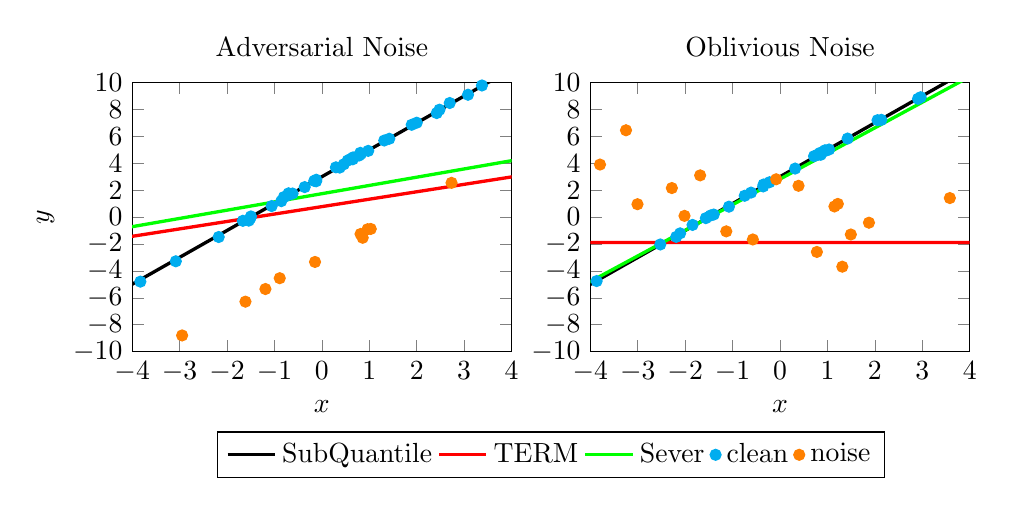
\begin{tikzpicture}
			\begin{groupplot}[group style={group size= 2 by 4},height=5cm,width=6.4cm,xmax=4,xmin=-4,
				ymin= -10,ymax=10,
				xtick={-4,-3,-2,...,4},
				ytick={-10,-8,-6,...,10},]
				\nextgroupplot[title=Adversarial Noise,ylabel={$y$},xlabel={$x$}]
				\coordinate (c1) at (current axis.left of origin);
				\addplot[mark=*,color=cyan,only marks] coordinates{(0.5454756141119426,4.20207144062236) (2.6952740390873733,8.475671650669172) (-0.1612438784423731,2.688323570846449) (1.9998807196500725,7.011477368661404) (0.6573126643085468,4.432503359641061) (0.822541876079238,4.691099695987436) (-1.665736406528514,-0.2771610262088303) (0.2955820690953599,3.6958661148678047) (4.329988449821567,11.633259356797302) (-4.412313203501535,-5.77063957797815) (3.5629538644332275,10.091868592245838) (-0.6175885445775965,1.7473187369931718) (0.8108793561773843,4.772417668204566) (1.4214273053887914,5.818934958869865) (3.081315566792172,9.08926804908307) (-0.12089034451099817,2.6605946971138144) (0.4628376617792958,3.923002461330265) (0.37617729415550505,3.676581100428469) (0.977114787165429,4.918947422974899) (1.314754156260769,5.688804682122404) (-0.36235424331683597,2.2267827837116263) (-0.8007556950385752,1.4886373858967947) (-0.7015664550907283,1.7651694045148667) (-2.1753647987904734,-1.482231084924366) (-1.495574696589605,0.04857682714064265) (-1.0588112744961395,0.8183551891451499) (-3.827119610541674,-4.796523392389788) (-0.8559789159750391,1.1837704089349095) (-0.11761120022533014,2.7730611413376285) (3.3752350984949295,9.778804511993851) (2.4222770389407957,7.727148811092623) (-1.5410032016624133,-0.2633438113497304) (2.480017633230306,7.979402356067379) (0.5911583134769168,4.283748748593926) (-0.71501674964969,1.6324881095139794) (0.6516043112113717,4.294631666773893) (-3.079711134644328,-3.285226613281087) (-1.5088703031224757,-0.08081402676688078) (0.7827672445662932,4.570750601954812) (1.8939059587103262,6.858172766747038)};
				\addplot[mark=*,color=orange,only marks] coordinates{(-2.946629011640607,-8.793723527498958) (0.8607384957406246,-1.538989556510056) (-1.1903001477494382,-5.345751610044574) (1.0305878148541996,-0.8812658035679226) (2.7345343942849927,2.5442143953062244) (-1.6113746066635852,-6.284678207630399) (-0.8883952236652384,-4.5410943399901775) (0.8157297797465353,-1.2566730413348421) (0.9642301396642339,-0.9032576567416104) (-0.14448993411816005,-3.334946134068381)};
				\addplot[domain=-5:5,samples=120,color=black,very thick] {1.99804993*x+2.99972117} ;
				\addplot[domain=-5:5,samples=120,color=red,very thick] {0.55184722*x+0.77673256} ;
				\addplot[domain=-5:5,samples=120,color=green,very thick] {0.61291924*x+1.73788515} ;
				\nextgroupplot[title=Oblivious Noise,xlabel={$x$},legend to name={IntroLegend},legend style={legend columns=5}]
				\coordinate (c2) at (current axis.right of origin);% I moved this to the upper right corner
				\addplot[domain=-5:5,samples=120,color=black,very thick] {2.00041502*x+3.00091281} ;
				\addlegendentry{SubQuantile}
				\addplot[domain=-5:5,samples=120,color=red,very thick] {0.000166177232*x-1.89493121} ;
				\addlegendentry{TERM}
				\addplot[domain=-5:5,samples=120,color=green,very thick] {1.90359844*x+2.82276139} ;
				\addlegendentry{Sever}
				\addplot[mark=*,color=cyan,only marks] coordinates{(0.788762485297498,4.619409754983769) (-1.8444557076323929,-0.5824544981134812) (-3.8667186653234786,-4.754991283615981) (-1.0770702633013416,0.7722164021812354) (-0.35460032498749144,2.2768627851664966) (-6.0822151692288084,-9.06286764938399) (-1.3972518211012221,0.1885381821988659) (2.9097896507970673,8.788974171667162) (-0.3463437020806441,2.420626808504963) (-2.1062359514012012,-1.2085000641078332) (4.336773668705573,11.632780878244247) (-0.6106102670869219,1.8184898177512854) (2.964822961712252,8.905021515559394) (-1.5637145371389622,-0.07761865537709459) (1.0345144344033383,5.0204590940620575) (2.056356483528722,7.198480210723839) (-0.7446791767339869,1.5853174482562558) (0.9631985535487033,4.9300987804715914) (0.8591431516732644,4.6302171243067765) (2.136527593488855,7.225942702339085) (-0.22230647531299189,2.5877920816746207) (1.4255477338524918,5.833868092502212) (-1.4608390115429133,0.12305693654859831) (0.8455335501589681,4.769483861326801) (-2.1885026970448886,-1.4714423105566306) (0.31837311592194245,3.604291796660203) (-2.5244214783210617,-2.0353095069267404) (0.9463907944621844,4.957203119009067) (0.8146787696108556,4.669681514124957) (0.7171745412553174,4.525279797042462)};
				\addlegendentry{clean}
				\addplot[mark=*,color=orange,only marks] coordinates{(-3.2474795820658593,6.450035960386647) (1.8753826722797218,-0.41858598306318395) (1.4931353198669002,-1.2946095099790276) (-6.390816833283051,0.40645831126308823) (0.39048632994899735,2.323962397589362) (-0.08068388106259215,2.8091622671588747) (1.3134080902531131,-3.6866845075408796) (-0.5728261692279717,-1.6637925896534693) (-3.795620644314326,3.901941933326407) (-2.2805802625691634,2.1567188534369586) (-1.1331317978018236,-1.0620378556289347) (-4.057270733769615,6.22788036393642) (3.580927646622491,1.4134339560728868) (1.1473909216831844,0.7892374536150136) (4.60155271303633,1.1396713973323012) (0.777450139132804,-2.5904275309220073) (1.2193257645912936,0.9783812850138183) (-2.0137550195781966,0.08990758847097716) (-3.0052924293950043,0.9558207339897568) (-1.6843214424199917,3.0989236738078767)};
				\addlegendentry{noise}
			\end{groupplot}
			\coordinate (c3) at ($(c1)!.5!(c2)$);
			\node[below] at (c3 |- current bounding box.south)
				{\pgfplotslegendfromname{IntroLegend}};
		\end{tikzpicture}
		\caption{Sub-Quantile Performance on Adapative Outliers}
		\label{fig:structure-unstructured-noise}
	\end{figure}
	
	As seen in the above comparison, current models fail to estimate data sets corrupted by structured noise, with some models even failing to estimate trends plagued with unstructured noise. Through this, sub-quantile optimization is shown to prevail at overcoming these challenges current models currently face. In Table 
	
	\begin{table}[!h]
		\centering
		\begin{tabular}{lcc}
			\toprule 
			Paper & Adversary & Threshold\\   
			\midrule                
			Sever \cite{DiakonikolasKKLSS19} & Adaptive & Gradient of Loss \\
			\midrule
			CRR \cite{bhatia2017} & Oblivious & \\
			\midrule 
			This Paper & Adapative & Loss\\
			\bottomrule
		\end{tabular}
		\caption{A comparison of different iterative thresholding algorithms for Robust Least Squares Regression}
		\label{tab:related-work}
	\end{table}
	
	\section{Related Work}
	Least Trimmed Squares (LTS) \cite{LTS} is an estimator that relies on minimizing the sum of the smallest $h$ residuals given a $(d-1)$-dimension hyperplane calculated given $n$ data points in $\mathbf{R}^d$ and an integer trimming parameter $h$. Given that the outliers comprise less than half the data, this algorithm is more efficient than the more common LMS estimator. However, this algorithm unfortunately suffers from the curse of dimensionality; the computational cost of the algorithm grows exponentially with increasing dimensions of the data. Thus, the necessity to design a more computationally efficient algorithm is expressed.
	
	Tilted Empirical Risk Minimization (TERM) \cite{li2020tilted} is a framework built to similarly handle the shortcomings of emperical risk minimization (ERM) with respect to robustness. The TERM framework instead minimizes the following quantity, where $t$ is a hyperparameter known as tilt
	\begin{equation}
		\tilde{R}(t;\vtheta) \coloneqq \frac{1}{t} \log\left(\frac{1}{N}\sum_{i \in \left[N\right]}e^{tf(\vx_i;\vtheta)} \right)
	\end{equation}
	By using the tilt hyperparameter to change the individual impact of each specific loss, the model is more resistant to outliers found in the data.
	
	SMART \cite{https://doi.org/10.48550/arxiv.2206.04777} proposes the \textit{iterative trimmed maximum likelihood estimator} against adversarially corrupted samples in General Linear Models (GLM). The estimator is defined as follows, where $S = \{(\vx_i,y_i)\}_{i=1}^n$ represents the training data. \vspace{1em}
	\begin{equation}
		\hat{\vtheta}(S) = \min_{\vtheta} \min_{\hat{S} \subset S, |\hat{S}| = (1-\eps)n} \sum_{(\vx_i,y_i) \in S} -\log f(y_i|\vtheta^T\vx_i)
	\end{equation}
	This estimator is proven to return near-optimal risk on a variety of linear models, including Gaussian regression, Poisson regression, and binomial regression; these achievements can be demonstrated on label and covariate corruptions.
	
	
	SEVER \cite{DiakonikolasKKLSS19} is a gradient filtering algorithm which removes elements whose gradients have the furthest distance from the average gradient of all points
	\begin{equation}
		\tau_i = \left((\nabla f_i(\vw) - \hat{\nabla})\cdot \vv\right)^2
	\end{equation}
	This method is novel in that it is highly scalable, making it robust against high-dimension data with structured outliers. Similarly, SEVER is easily implemented with standard machine learning libraries and can be applied to many typical learning problems, including classification and regression. Despite this, the algorithm still falls short when features have high covariance or when features have low predictive power of the target. Moreover, SEVER requires approximate learners to be run after every iteration, making SEVER unfeasible for large-scale machine learning tasks. 
	
	Quantile Regression \cite{yu_quantile_2003} relies on splitting data into quantiles to better represent data that is not evenly distributed. The paper introduces various estimation methods for quantile regression and apply them to a multitude of datasets. In doing so, they prove quantile regression is suitable at estimating both linear and nonlinear response models.
	
	Super-Quantile Optimization \cite{ROCKAFELLAR2014140} aims to solve error minimization problems by building upon the aforementioned quantile regression by centering around a conditional value-at-risk, or a superquantile. For $\alpha \in [0,1)$, the $\alpha$-superquantile for a random variable $Y$ is defined as \begin{equation}
		\Bar{q}_\alpha (Y) := \frac{1}{1-\alpha} \int_\alpha^1 q_\beta (Y) d\beta
	\end{equation}
	In doing so, more conservatively fitted curves are produced. As with quantile regression, such curves do require the solution of a linear program.
	This concept of superquantile error provides insight into tail behavior for quantities of error and an overall unique approach to linear regression.
	
	Robust Risk Minimization \cite{RRM} is a method in which given an upper bound on the corrupted data fraction $\epsilon$, the risk function can be minimized as follows:
	\begin{equation}
		\hat{\mathbb{\theta}}_{RRM} = \operatorname*{argmin}_{\theta \in \Theta} \operatorname*{min}_{\pi \in \Pi: \mathbf{H}(\pi) \geq ln|(1-\tilde{\epsilon})n|} R(\mathbb{\theta,\pi})
	\end{equation}
	This method is popular as it does not require the removal of corrupted data points and does not rely on a specified corruption fraction.
		
	\section{Sub-quantile Optimization}
	\label{sec:sub-quantile-optimization}
	
	\begin{definition}
		Let $F_X$ represent the Cumulative Distribution Function (CDF) of the random variable $X$. The \textbf{$\mathbf{p}$-Quantile} of a Random Variable $X$ is defined as follows \vspace{1em}
		\begin{equation}
			Q_p(p) = \inf\{x\in\mathbb{R}: p \leq F(x)\} 
		\end{equation}
	\end{definition}
	
	\begin{definition}
		Let $\ell$ be the loss function. \textbf{Risk} is defined as follows
		\begin{equation}
			U = \mathbb{E}_{(\vx,y) \sim \mathbb{P}}\left[\ell \left( f(\vx;\vtheta,y)\right)\right]
		\end{equation}
	\end{definition}
	The $\mathbf{p}$-\textbf{Quantile} of the Empirical Risk is given
	\begin{equation}\label{eqn:sub-quantile}
		\mathbb{L}_p(U) = \frac{1}{p}\int_0^p \mathcal{Q}_q(U)\,dq = \mathbb{E}\left[U|U \leq \mathcal{Q}_p(U) \right] = \max_{t\in \mathbb{R}}\left\{t - \frac{1}{p}\mathbb{E}\left[(t-U)^+\right]\right\}
	\end{equation}
	In equation \ref{eqn:sub-quantile}, $t$ represents the $p$-quantile of $U$. We also show that we can calculate $t$ by a maximizing optimization function. 
	The Sub-Quantile Optimization problem is posed as follows
	\begin{equation}
		\vtheta_{SM} = \argmin_{\vtheta \in \mathbb{R}^d} \max_{t \in \mathbb{R}} \left\{t - \frac{1}{p}\mathbb{E}(t - \ell(f(\vx;\vtheta),y))^+\right\}
	\end{equation}
	
	For the linear regression case, this equation becomes 
	\begin{equation}
		\label{eqn:theta_sm}
		\vtheta_{SM} = \argmin_{\vtheta \in \mathbb{R}^d} \max_{t \in \mathbb{R}} \left\{t - \frac{1}{np}\sum_{i=1}^n(t-(\vtheta^T\vx_i - y_i)^2)^+\right\}
	\end{equation}
		
	The two-step optimization for Sub-Quantile optimization is given as follows \vspace{1em}
	\begin{equation}
		\label{eqn:t-update}
		t_{k+1} = \argmax_t g(t,\vtheta_k) 
	\end{equation}
	\begin{equation}
		\label{eqn:theta-update}
		\vtheta_{k+1} = \vtheta_k + \alpha \nabla_{\vtheta_k} g(t,\vtheta_k)
	\end{equation}
		
	This algorithm is adopted from \cite{Razaviyayn}. Theoretically, it has been proven to converge in research by \cite{Jin_2019}.\\
	\begin{minipage}{0.48\textwidth}
	\begin{algorithm}[H]
		\DontPrintSemicolon
		
		\KwInput{Training iterations $T$, Quantile $p$, SubQuantile Update: $j$}
		\KwOutput{Trained Parameters, $\displaystyle \vtheta_{(T)}$}
		$\vtheta_{(0)} \gets (X^T X)^{-1}X^T y$\\
		\For{$k \in 1,2,\ldots,T$}
		{
			$\displaystyle \vnu \gets \left(X\vtheta_{(k)} - y\right)^2$\\
			\If{$k \% j = 0$}
			{
				$\hat{\vnu} \gets sorted(\vnu)$\\
				$\displaystyle t_{(k+1)} \gets \hat{\vnu}_{np}$\\
			}
			$S_{(k)} \gets \concat \vx_i\text{ if } (\vtheta_{(k)}^T \vx_i - y_i)^2 \leq t_{(k+1)}$\\
			$L_{(k)} \gets \frac{1}{np}\norm{S^T S}_2$\\
			$\alpha_{(k)} \gets \frac{1}{2L_{(k)}}$\\
			$\displaystyle \vtheta_{(k+1)} \gets \vtheta_k - \alpha_{(k)} \nabla_\vtheta g(t_{(k+1)},\vtheta_{(k)})$
		}
		\KwRet{$ \vtheta_T $}
		\caption{Sub-Quantile Minimization Gradient Descent}
		\label{alg:sqo1}
	\end{algorithm}
	\end{minipage}
	\hfill
	\begin{minipage}{0.48\textwidth}
		\begin{algorithm}[H]
			\KwInput{Training Iterations $T$,Quantile $p$}
			\KwOutput{Trained Parameters, $\vtheta_{(T)}$}
			$\vtheta_{(0)} \gets (X^T X + \lambda I)^{-1}X^T y$\\
			\For{$k \in \left\{1,2,\dots,T\right\}$}
			{
				$\vnu \gets (X \vtheta_{(k)} - y)^2$\\
				$t_{(k+1)} \gets \hat{\vnu}_{np}$\\
				$S_{(k)} \gets \concat \vx_i\text{ if } (\vtheta_{(k)}^T \vx_i - y_i)^2 \leq t_{(k+1)} \text{ where $\concat$ represents the concatenation operator}$\\
				$\vtheta_{(k+1)} \gets (S^T S + \lambda I)^{-1}S^T y_S$\\
			}
			\KwRet{$ \vtheta_T $}
			\caption{Sub-Quantile Minimization for Ridge Regression}
			\label{alg:sqo-ridge}
		\end{algorithm}
	\end{minipage}
		
	\subsection{Motivation}
	\begin{assumption}\label{asm:normal-corruption}
		To provide theoretical bounds on the effectiveness of Sub-Quantile Minimization, we make the General Linear Model Assumption that
		\begin{equation}\vspace{1em}
			\vy_P = P\vbeta_P  + \eps_P
		\end{equation}
		and similarly 
		\begin{equation}
			\vy_Q = Q \vbeta_Q + \eps_Q
		\end{equation}
		where $\vbeta_P$ and $\vbeta_Q$ the \textit{oracle} regressors for $\mathbb{P}$ and $\mathbb{Q}$ and $\eps_P$ and $\eps_Q$ are both Normally Distributed with mean $0$.  
	\end{assumption}
	Since we are interested in learning the optimal model for distributions, our goal is to learn the parameters $\vbeta_P$ from the distribution $\hat{P}$. We want to clarify the corruption is not adversarially chosen. \\
	In this section we quantify the effect of corruption on the desired model. To introduce notation, let $P$ represent the data from distribution $\mathbb{P}$ and let $Q$ represent the training data for $\mathbb{Q}$. Let $\vy_P$ represent the target data for $\mathbb{P}$ and let $\vy_Q$ represent the target data for $\mathbb{Q}$.\\
	\begin{assumption}\label{asm:p-q-sample}
		We assume the rows of $P$ and $Q$ are sampled from the same multivariate normal distribution. \vspace{1em}
		\begin{equation}
			P_i,Q_j \sim \mathcal{N}_p(\mathbf{0},\Sigma)
		\end{equation}
	\end{assumption}
	
	We will use our assumptions to quantify the effect of the corrupted data on an optimal least squares regression model. We are interested in $\displaystyle (X^T X)^{-1}X^T y - (P^T P)^{-1}P^T y$.
	It is know the least squares optimal solution for $X$ is equal to $(X^T X)^{-1}X^T y$\\
	Note $\displaystyle X = \begin{pmatrix}P \\ Q \end{pmatrix}$ and $\displaystyle y = \begin{pmatrix} \vy_P \\ \vy_Q \end{pmatrix} $so $X^T = \begin{pmatrix}P^T & Q^T \end{pmatrix}$\\
	
	\begin{restatable}{thm}{expected-value-corrupted}\label{thm:expected-value-corrupted}
		The expected optimal parameters of the corrupted model $\hat{\mathbb{P}}$\vspace{1em}
		\begin{equation}
			\label{eqn:corrupted-optimal}
			\mathbb{E}\left[X^{\dagger}y \right] = \vbeta_P + \eps(\vbeta_Q - \vbeta_P)
		\end{equation}
	\end{restatable}
	The proof is reliant on assumption \ref{asm:p-q-sample}, this allows us to utilize the Wishart Distribution, $\mathcal{W}$, and the inverse Wishart Distribution, $\mathcal{W}^{-1}$. Please refer to Appendix \ref{app:expected-value-corrupted}. By Theorem \ref{thm:expected-value-corrupted} we can see the level of corruption is dependent upon $\eps$, which represents the percentage of corrupted samples, and the distance between the optimal parameters for $\mathbb{P}$, which is $\vbeta_P$ and the optimal parameters for $\mathbb{Q}$, which is $\vbeta_Q$. 
	
		
	Here we utilize the idea of \textit{influence} from \cite{McWilliams2014}.
	
	Theorem \ref{thm:expected-value-corrupted} finds the optimal model when the corrupted distribution is sampled from the same distribution as the target distribution but has different optimal parameters. We will now look at the case of feature corruption. This is where the optimal parameters of the two distributions are the same but the data from $\mathbb{P}$ and $\mathbb{Q}$ are sampled differently. 
	
	In equation \ref{eqn:corrupted-optimal}, note as $\displaystyle \eps \to 0$ we are returned $\vbeta_P$. This is the intuition behind SubQuantile Minimization. By minimizing over the SubQuantile, we seek to reduce $\eps$, and thus our model will return a model which is by expectation closer to $\vbeta_P$. 	

	\section{Theory} 
	
	\subsection{Analysis of $g(t,\theta)$}
	
	In this section, we will explore the fundamental aspects of $g(t,\vtheta)$. This will motivate the convergence analysis in the next section.
	
	\begin{restatable}{lemma}{gtconcavelemma}
		\label{lem:gtcomcavelemma}
		$g(t_{k+1},\vtheta_k)$ is concave with respect to $t$.
	\end{restatable}
	\begin{proof}
		We provide a simple argument for concavity. Note $t$ is a concave and convex function. Also $(\cdot)^+$ is a convex strictly non-negative function. Therefore we have a concave function minus the non-negative multiple of a summation of an affine function composed with a convex function. Therefore this is a concave function with respect to $t$. 
	\end{proof}	
	
	\begin{restatable}{lemma}{gfermat}
		\label{lem:gfermat}
		The maximizing value of $t$ in $g(t,\vtheta)$ in $t$-update step of optimization as described by Equation \ref{eqn:t-update} is maximized when $t = Q_p(U)$
	\end{restatable}
		\begin{proof}
		Since $\displaystyle g(t,\vtheta)$ with respect to $t$ is a concave function. Maximizing $g(t,\vtheta)$ is equivalent to minimizing $-g(t,\vtheta)$. We will find fermat's optimality condition for the function $\displaystyle -g(t,\vtheta)$, which is convex. 
		Let $\displaystyle \hat{\vnu} = sorted\left((\vtheta^T X - y)^2\right)$ and note $\displaystyle 0 < p < 1$
		\begin{align}
			\partial{\displaystyle (-g(t,\boldsymbol{\theta}})) 
			&= -1 + \frac{1}{np}\sum_{i=1}^{n}
			\left\{
			\begin{array}{lr}
				1, & \text{if } t > \hat{\vnu}_i\\
				0, & \text{if } t < \hat{\vnu}_i \\
				\left[0,1\right], & \text{if } t = \hat{\vnu}_i \\
			\end{array}
			\right\}&&\\
			&= 0 \text{ when }\displaystyle t = \hat{\vnu}_{np}&&
		\end{align}
		This is the $p$-quantile of $U$. A full proof is provided in Appendix \ref{app:gfermat}.
	\end{proof}
	
	\begin{restatable}{lemma}{gthetaderiv}\label{lem:gthetaderiv}
		Let $t = \hat{\vnu}_{np}$. The $\vtheta$-update step described in Equation \ref{eqn:theta_sm} is equivalent to minimizing the least squares loss of the $np$ elements with the lowest squared loss.
	   \begin{equation}
			\nabla_{\vtheta}g(t_{k+1},\vtheta_k) = \frac{1}{np}\sum_{i=1}^{np}2\vx_i(\vtheta_k^T\vx_i - y_i)
		\end{equation}
	\end{restatable}
	We provide a proof in Appendix \ref{app:gthetaderiv}. However, this result is quite intuitive as it shows we are optimizing over the $p$ Sub-Quantile of the Risk.
	\begin{interpretation}
		\label{int:minimize-small}
		Sub-Quantile Minimization continously minimizes the risk over the $p$-quantile of the error. In each iteration, this means we reduce the error of the points within the lowest $np$ errors.
	\end{interpretation}

		
	\begin{restatable}{lemma}{gthetaconvexlemma}
		\label{lem:gthetaconvex}
		$g(t_{k+1},\vtheta_k)$ is convex with respect to $\vtheta_k$.
	\end{restatable}
	\begin{proof}
		We see by lemma \ref{lem:gfermat} and interpretation \ref{int:minimize-small}, we are optimizing by the $np$ points with the lowest squared error. Mathematically, 
		\begin{align*}
			g(t_{k+1},\vtheta_k) &= t_{k+1} - \frac{1}{np}\sum_{i=1}^{n}\left(t_{k+1} - (\vtheta^T\vx_i - y_i)^2\right)^+ &&\\
			&= t - t + \frac{1}{np}\sum_{i=1}^{np}(\vtheta^T\vx_i - y_i)^2 &&\\
			&= \frac{1}{np}\sum_{i=1}^{np}(\vtheta^T\vx_i - y_i)^2 &&
		\end{align*}
		Now we can make a simple argument for convexity. We have a non-negative multiple of the sum of the composition of an affine function with a convex function. Thus $g(t,\vtheta)$ is convex with respect to $\vtheta$.
	\end{proof}
	
	\begin{restatable}{lemma}{g-lsmooth}
		\label{lem:g-lsmooth}
		$g(t,\vtheta)$ is $L$-smooth with respect to $\vtheta$ with $\displaystyle L = \norm{\frac{2}{np}\sum_{i=1}^{np}\norm{\vx_i}^2}$ 
	\end{restatable}
	
	Now we will state two properties regarding the effect of the $t$-update step and the $\vtheta$-update step as described in Equations \ref{eqn:t-update} and \ref{eqn:theta-update}, respectively. 
	\begin{restatable}{lemma}{g-change-wrt-t}
		\label{lem:g-change-wrt-t}
		If $t_{k+1} \leq t_k$ then $ g(t_{k+1},\vtheta_k) = g(t_{k}) + \frac{1}{np}\sum_{i=np}^n(t_k - \vnu_i)^+$. If $t_{k+1} > t_k$, then $ g(t_{k+1},\vtheta_k) = g(t_k) + \frac{1}{np}\sum_{i=n(p-\delta)}^{np}(t-\vnu_i)^+  - \delta t$. For a small $\delta$. 
	\end{restatable}
	\begin{proofsketch}
		When $t_{k+1} \leq t_k$ this result is quite intuitive, as we are simply removing the error of the elements outside elements within the lowest $np$ squared losses. We delegate the rest of the proof to Appendix \ref{app:g-change-wrt-t}
	\end{proofsketch}

	\subsection{Optimization}

	We are solving a min-max convex-concave problem, thus we are looking for a Nash Equilibrium Point. 
	
	\begin{restatable}{definition}{nash-equilibrium}
		\label{def:nash-equilibrium}
		$(t^*,\vtheta^*)$ is a \textbf{Nash Equilibrium} of $g$ if for any $(t,\vtheta) \in \mathbb{R}\times\mathbb{R}^d$\vspace{1em}
		\begin{equation}
			g(t^*,\vtheta) \leq g(t^*,\vtheta^*) \leq g(t,\vtheta^*)
		\end{equation}
	\end{restatable}	
	\begin{restatable}{definition}{local-nash-equilibrium}
		\label{def:local-nash-equilibrium}
		$(t^*,\vtheta^*)$ is a \textbf{Local Nash Equilibrium} of $g$ if there exists $\delta > 0$ such that for any $t,\vtheta$ $(t,\vtheta)$ satsifying $\norm{t - t^*} \leq \delta$ and $\norm{\vtheta -\vtheta^*} \leq \delta$ then: 
		\vspace{1em}
		\begin{equation}
			g(t^*,\vtheta) \leq g(t^*,\vtheta^*) \leq g(t,\vtheta^*)
		\end{equation}
	\end{restatable}
	\begin{proposition}\label{prop:first-order-nash}
		As $g$ is first-order differentiable,  any local Nash Equilibrium satisfies $\nabla_\vtheta g(t,\vtheta) = \mathbf{0}$ and $\nabla_t g(t,\vtheta) = 0$
	\end{proposition}
	
	We are now interested in what it means to be at a Local Nash Equilibrium. By Proposition \ref{prop:first-order-nash}, this means both first-order partial derivatives are equal to $0$. By lemma \ref{lem:gfermat}, we have shown $\nabla_tg(t,\vtheta) = 0$ when $\vnu_{np} \leq t < \vnu_{np+1}$. Furthermore, by lemma \ref{lem:gthetaderiv}, we have shown $\nabla_\vtheta(g,\vtheta) = 0$ when the least squares error is minimized for the $np$ points with lowest squared error. In other words:
	\begin{align*}
		\mathbb{E}\left[\nabla_\vtheta g(t_{k+1},\vtheta_k)\right] &= 0 &&\\
		2(\vmu\vmu^T + \Sigma)(\vtheta_k - (1-\varepsilon)\vbeta_P-\varepsilon\vbeta_Q) &= 0&&
	\end{align*}
	Since the first term is non-zero, the equality is satisfied when:
	\begin{equation*}
		(\vtheta_k - (1-\varepsilon)\vbeta_P-\varepsilon\vbeta_Q) = 0
	\end{equation*}	
	\begin{equation*}
		\vtheta_k = (1-\varepsilon)\vbeta_P + \varepsilon\vbeta_P 
	\end{equation*}
	Note this aligns with the results of Theorem \ref{thm:expected-value-corrupted}.
	This means that for a subset of $np$ points from $X$, the least squares error is minimized. What we are interested in is how many points within those $np$ points come from $\mathbb{P}$ and how many of those points from $\mathbb{Q}$. Our goal is to minimize the number of points within the $np$ lowest squared losses from $Q$, as they will introduce error to our predictions on points from $P$. 
	
	
	
	\begin{restatable}{thm}{convergence-guarantee}
		\label{thm:convergence-guarantee}
		Let $g(t,\vtheta)$ be differentiable and $g(t,\vtheta)$ be $L$-smooth in $\vtheta$. Let $t_{(k)}$ and $\vtheta_{(k)}$ be iterates from algorithm \ref{alg:sqo-ridge}. Then, $\lim_{k \to \infty} \mathbb{E}\left[\norm{\nabla_\vtheta g(t_{(k+1)},\vtheta_{(k)})}\right] = 0$.
	\end{restatable}
	\begin{proofsketch}
		From the intuitions we have gained on Subquantile Minimization. We can state the following:
		\begin{equation}
			\argmin_{\vtheta \in \mathbb{R}^d}\min_{S \in \Pi}\norm{\vtheta^T S - y_S}_2^2 \iff \argmin_{\vtheta \in \mathbb{R}^d}\max_{t \in \mathbb{R}}\norm{\vtheta^T S - y_S}_2^2
		\end{equation}
		where $\Pi$ represents the entire distribution of Subquantile matrices. 
	\end{proofsketch}
	

	\subsection{Converging to $\beta_P$}
	
	We will start by defining the two types of noise we are interesting in. 
	\begin{definition}
		\textbf{Oblivious Noise} is noise that is not dependent on the input data, i.e., $\displaystyle \mathbb{P}\left[y | X\right] = \mathbb{P}\left[y\right]$
	\end{definition}
	\begin{definition}
		\textbf{Adaptive Noise} is noise that is made from a linear combination of the input data, i.e. $\displaystyle y = \vbeta_QX + \veps$
	\end{definition}
	Also note we often consider Gaussian Noise as Oblivious Noise, but it can be modeled as Adaptive Noise where $\vbeta_Q = \vzero$. 

	\begin{restatable}{lemma}{effect-of-projection}
		\label{lem:effect-of-projection}
		The expected value of error on points in $\mathbb{P}$ will be lower than the expected value of error on points in $\mathbb{Q}$ if $\proj_{\vbeta_P}(\vtheta) - \vbeta_P < \proj_{\vbeta_Q}(\vtheta) - \vbeta_Q$
	\end{restatable}
	
	Lemma \ref{lem:effect-of-projection} gives us an intuitive result, the proof is in appendix \ref{app:effect-of-projection}. If in each optimization step, our projection on $\vbeta_P$ is closer than our projection on to $\vbeta_Q$, we know the number of steps from $\mathbb{Q}$ will increase from the previous iteration.
	\begin{restatable}{thm}{improvement-of-theta}
		\label{thm:improvement-of-theta}
		After an optimization step, 
		\begin{equation*}
			\left|\proj_{\vbeta_P}\vtheta_{(t+1)} -1 \right| - \left|\proj_{\vbeta_P}\vtheta_{(t)} -1 \right| <  \left|\proj_{\vbeta_Q}\vtheta_{(t+1)} - 1\right| - \left|\proj_{\vbeta_Q}\vtheta_{(t)} - 1\right|
		\end{equation*}
			  if the following holds
		\begin{equation}
			\norm{\left((1-\varepsilon^{(t)}) - \alpha_1\right)\vbeta_P} > \norm{\left(\varepsilon^{(t)} - \alpha_2\right)\vbeta_Q}
		\end{equation}
		where $\alpha_1$ and $\alpha_2$ represents the coefficients for the linear combination of $\vtheta$ in the basis defined as $\mB = \begin{bmatrix} \vbeta_P & \vbeta_Q & \mR\end{bmatrix}$
	\end{restatable}

	We are also interested in Algorithm \ref{alg:sqo-ridge}, so we provide theory for it.
	\begin{restatable}{corollary}{ridge-algorithm-convergence}
		\label{thm:ridge-algorithm-convergence}
		Theorem \ref{alg:sqo-ridge} by expectation converges to a good solution. 
	\end{restatable}
	\begin{proofsketch}
		Let us first note $\varepsilon^{(0)} < 0.5$, and by Theorem \ref{thm:expected-value-corrupted}, $\vtheta_{(0)} = (1-\varepsilon^{(0)})\vbeta_P + \varepsilon^{(0)}\vbeta_Q$. It thus follows:
		\begin{equation}
			\norm{\vtheta_{(0)} - \vbeta_P} = \norm{\varepsilon^{(0)}\vbeta_P + \varepsilon^{(0)}\vbeta_Q}
		\end{equation}
		and similarly 
		\begin{equation}
			\norm{\vtheta_{(0)} - \vbeta_Q} = \norm{(1 - \varepsilon^{(0)})\vbeta_P + (1 - \varepsilon^{(0)}) \vbeta_Q}
		\end{equation}
		Therefore in the linear case 
		\begin{equation}\label{eqn:theta-0-closer-to-p}
			\norm{\varepsilon^{(0)}\vbeta_P + \varepsilon^{(0)}\vbeta_Q} < \norm{(1 - \varepsilon^{(0)})\vbeta_P + (1 - \varepsilon^{(0)}) \vbeta_Q}
		\end{equation}
		Then if $\Var(\epsilon_P) \leq \Var(\epsilon_Q)$, it follows 
		\begin{equation*}
			\mathbb{E}\left[\left(\vtheta_{(0)}^T \vp - y_i\right)^2\right] \leq \mathbb{E}\left[\left(\vtheta_{(0)}^T \vq - y_i\right)^2\right]
		\end{equation*}	
		This concludes the proof.
	\end{proofsketch}
	
	Note theorem \ref{thm:ridge-algorithm-convergence} is enough to show the final subquantile matrix will have more elements from $P$. It thus follows, in the case of no feature noise, by expectation, $\vtheta$ will move towards $\vbeta_P$ faster than it moves to $\vbeta_Q$. We instead calculate the probability in theorem \ref{thm:probability-epsilon-decreasing}. 
	
	We are now interested in theoretical guarantees with no distributional assumptions. First we will consider some intuition on why this problem is not as hard as compared to when the corruption is linearly structured. Let us say the noise is of non-linear regression, in other words $\vy_Q \sim f(X,\vbeta_Q)$, where $f$ is a non-linear combination of features of $X$. In this case, it is not possible to model the non-linear regression by a linear combination of the features, thus, if we have elements from $\mathbb{Q}$ within the lowest $np$ losses, then training on these points will not generalize well to points from $\mathbb{Q}$, so their error will not decrease. 

	
	\section{Empirical Results}\label{sec:numerical-experiments}

	We also present a batch algorithm which improves training speed significantly. In accordance with Minibatch theory, if the subset $I$ of all data is representative of all the data, then this will have similar results to Algorithm \ref{alg:sqo1}.

	\subsection{Synthetic Data}
	
	\begin{figure}[!b]
		\centering
		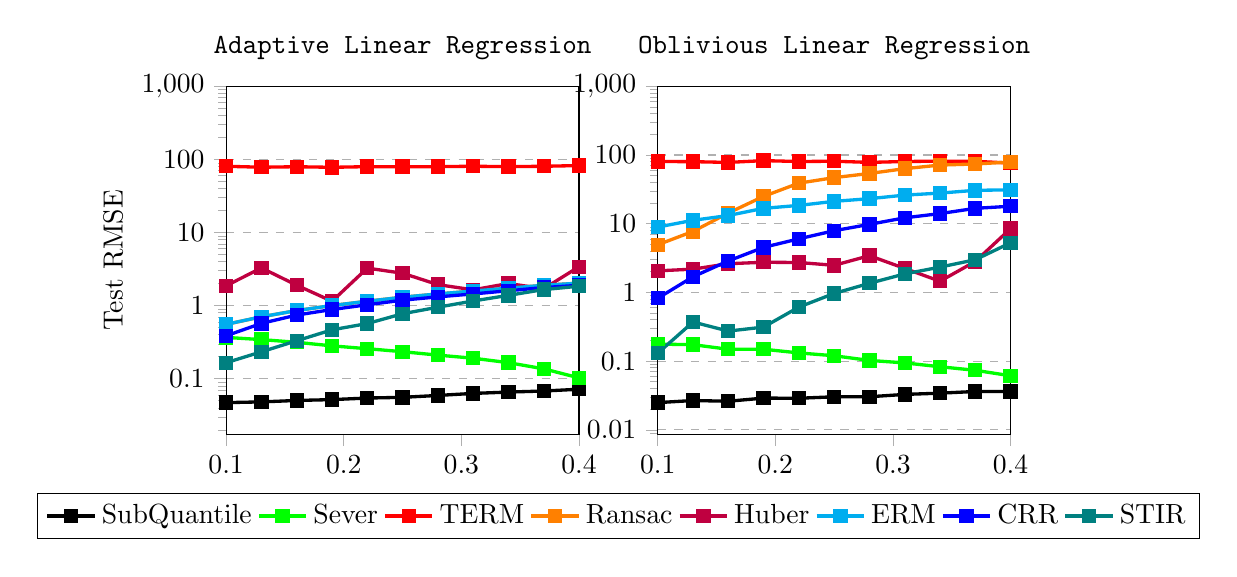
\begin{tikzpicture}
			\begin{groupplot}[group style={
					group name=myplot,
					group size= 2 by 1},height=6cm,width=0.5\linewidth,
					tick align=outside,
					tick pos=left,
					legend pos=outer north east,
					x grid style={darkgray176},
					xmin=0.1, xmax=0.4,
					xtick style={color=darkgray176},
					y grid style={darkgray176},
					ymin=0, ymax=1000,
					ytick style={color=darkgray176},
					ytick={0,0.001,0.01,0.1,1,10,100,1000},
					ymajorgrids=true,
					grid style=dashed,
					ymode=log,
					log ticks with fixed point,
				]
			\nextgroupplot[ylabel=Test RMSE,title=\texttt{Adaptive Linear Regression}]
			\coordinate (c1) at (current axis.left of origin);
			\addplot [very thick, black,mark=square*]
			table {%
				0.1 0.0470812581479549
				0.13 0.0481603480875492
				0.16 0.050400760024786
				0.19 0.0517568401992321
				0.22 0.0543827041983604
				0.25 0.0556097775697708
				0.28 0.0590417385101318
				0.31 0.0629159957170486
				0.34 0.0656534433364868
				0.37 0.06785549223423
				0.4 0.0717944204807281
			};
			\addplot [very thick, green,mark=square*]
			table {%
				0.1 0.36738908290863
				0.13 0.342920124530792
				0.16 0.314845204353333
				0.19 0.28143972158432
				0.22 0.257287442684174
				0.25 0.234187826514244
				0.28 0.210285276174545
				0.31 0.190747454762459
				0.34 0.165870726108551
				0.37 0.136498242616653
				0.4 0.102688848972321
			};
			\addplot [very thick, red,mark=square*]
			table {%
				0.1 80.540153503418
				0.13 78.2785491943359
				0.16 79.4500045776367
				0.19 78.0468368530273
				0.22 79.6445236206055
				0.25 79.5632705688477
				0.28 79.6250457763672
				0.31 80.7044982910156
				0.34 79.593620300293
				0.37 80.6381225585938
				0.4 82.4261169433594
			};
			\addplot [very thick, orange,mark=square*]
			table {%
				0.1 0.55393660068512
				0.13 0.702713727951059
				0.16 0.8559549450874336
				0.19 1.00228035449982
				0.22 1.14807796478271
				0.25 1.30311346054077
				0.28 1.44514167308807
				0.31 1.58323192596436
				0.34 1.73416042327881
				0.37 1.8974506855011
				0.4 2.0302050113678
			};
			\addplot [very thick, purple,mark=square*]
			table {%
				0.1 1.87000024318695
				0.13 3.27856779098511
				0.16 1.90161323547363
				0.19 1.14748334884644
				0.22 3.25915050506592
				0.25 2.77480888366699
				0.28 1.93823385238647
				0.31 1.64351272583008
				0.34 2.00752592086792
				0.37 1.70363962650299
				0.4 3.40018320083618
			};
			\addplot [very thick, cyan,mark=square*]
			table {%
				0.1 0.554642379283905
				0.13 0.703209280967712
				0.16 0.856137990951538
				0.19 1.00242388248444
				0.22 1.1481751203537
				0.25 1.30330908298492
				0.28 1.44537603855133
				0.31 1.58298897743225
				0.34 1.73431789875031
				0.37 1.89734447002411
				0.4 2.03032040596008
			};
			\addplot [very thick, blue,mark=square*]
			table {%
				0.1 0.386876940727234
				0.13 0.571252167224884
				0.16 0.743153214454651
				0.19 0.883608460426331
				0.22 1.02778625488281
				0.25 1.1869922876358
				0.28 1.31735336780548
				0.31 1.44525456428528
				0.34 1.59675407409668
				0.37 1.76741755008698
				0.4 1.89613056182861
			};
			\addplot [very thick, teal,mark=square*]
			table {%
				0.1 0.165539637207985
				0.13 0.233492165803909
				0.16 0.330621749162674
				0.19 0.466441482305527
				0.22 0.568290293216705
				0.25 0.774224400520325
				0.28 0.951132595539093
				0.31 1.15776085853577
				0.34 1.3817971944809
				0.37 1.6569504737854
				0.4 1.84088504314423
			};
			\nextgroupplot[legend to name={CommonLegend},legend style={legend columns=8},title=\texttt{Oblivious Linear Regression}]
			\coordinate (c2) at (current axis.right of origin);
			\addplot [very thick, black,mark=square*]
			table {%
				0.1 0.0248506348580122
				0.13 0.0266600362956524
				0.16 0.0260318480432034
				0.19 0.0289147105067968
				0.22 0.0287831928580999
				0.25 0.0302000977098942
				0.28 0.0302627310156822
				0.31 0.0327312126755714
				0.34 0.0341136306524277
				0.37 0.0361219607293606
				0.4 0.0360446088016033
			};\addlegendentry{SubQuantile}
			\addplot [very thick, green,mark=square*]
			table {%
				0.1 0.176778882741928
				0.13 0.173329889774323
				0.16 0.148729845881462
				0.19 0.14880645275116
				0.22 0.131500840187073
				0.25 0.119577743113041
				0.28 0.102301254868507
				0.31 0.0941185131669044
				0.34 0.0827301070094109
				0.37 0.0734678506851196
				0.4 0.0611478313803673
			};\addlegendentry{Sever}
			\addplot [very thick, red,mark=square*]
			table {%
				0.1 80.537727355957
				0.13 80.0273361206055
				0.16 78.0828552246094
				0.19 82.857292175293
				0.22 80.457160949707
				0.25 81.2084121704102
				0.28 78.1319122314453
				0.31 80.4724807739258
				0.34 81.4710922241211
				0.37 80.9352798461914
				0.4 76.3578338623047
			};\addlegendentry{TERM}
			\addplot [very thick, orange,mark=square*]
			table {%
				0.1 4.93412590026855
				0.13 7.72555828094482
				0.16 14.3062973022461
				0.19 25.0096282958984
				0.22 38.9553298950195
				0.25 46.8739929199219
				0.28 53.8878555297852
				0.31 63.2952194213867
				0.34 71.4158630371094
				0.37 74.0310897827148
				0.4 79.1682586669922
			};\addlegendentry{Ransac}
			\addplot [very thick, purple,mark=square*]
			table {%
				0.1 2.05954170227051
				0.13 2.18071556091309
				0.16 2.61477184295654
				0.19 2.74768042564392
				0.22 2.72520542144775
				0.25 2.4791693687439
				0.28 3.42575645446777
				0.31 2.23458814620972
				0.34 1.45350193977356
				0.37 2.8192400932312
				0.4 8.48482227325439
			};\addlegendentry{Huber}
			\addplot [very thick, cyan,mark=square*]
			table {%
				0.1 8.94177627563477
				0.13 11.2084474563599
				0.16 13.1594343185425
				0.19 16.7554378509521
				0.22 18.4683818817139
				0.25 21.1728744506836
				0.28 23.1441192626953
				0.31 26.084171295166
				0.34 27.9081382751465
				0.37 30.6380157470703
				0.4 31.126895904541
			};\addlegendentry{ERM}
			\addplot [very thick, blue,mark=square*]
			table { 
				0.1 0.820617198944092
				0.13 1.68926250934601
				0.16 2.87315225601196
				0.19 4.52729034423828
				0.22 6.02502059936523
				0.25 7.91049146652222
				0.28 9.78747940063477
				0.31 12.1807632446289
				0.34 14.0376138687134
				0.37 16.7470684051514
				0.4 17.964750289917
			};\addlegendentry{CRR}
			\addplot [very thick, teal,mark=square*]
			table { 
				0.1 0.130227774381638
				0.13 0.370556622743607
				0.16 0.273394376039505
				0.19 0.312625408172607
				0.22 0.610911905765533
				0.25 0.965445756912231
				0.28 1.35678029060364
				0.31 1.85954880714417
				0.34 2.33366990089417
				0.37 2.99191808700562
				0.4 5.27555418014526
			};\addlegendentry{STIR}
			\end{groupplot}
			\coordinate (c3) at ($(c1)!.5!(c2)$);
			\node[below] at (c3 |- current bounding box.south)
			{\pgfplotslegendfromname{CommonLegend}};
		\end{tikzpicture}
		\caption{\texttt{Structured Linear Regression} \& \texttt{Noisy Linear Regression} Datasets}
		\label{fig:synthetic-linear-regression}
	\end{figure}
	We now demonstrate SubQuantile Regression in the presence of Gaussian Random Noise. 
		
	In our first synthetic experiment, we run Algorithm \ref{alg:sqo1} on synthetically generated structured linear regression data, the noise is sampled from a linear distribution that is dependent on the vector of $X$. Our results show the near optimal performance of Sub-Quantile Minimization. The results and comparison with other methods can be seen in Table \ref{tab:quadratic-regression}. We see in Table \ref{tab:quadratic-regression}, Sub-Quantile Minimization produces State of the Art Results in the Quadratic Regression Case. Furthermore, it performs significantly better than baseline methods in the high-noise regimes $(\eps = 0.4)$, this is confirmed in both the small data and large data datasets. Please refer to Appendix \ref{app:experimental-details} for more details on the \texttt{Structured Linear Regression} Dataset. 

	\subsection{Real Data}
	
	We provide results on the \texttt{Drug Discovery} Dataset in \cite{DiakonikolasKKLSS19} utilizing the noise procedure described in \cite{li2020tilted}. For each algorithm, if possible we use Ridge Regression, else we use typical least squares. SubQuantile Minimization, ERM, RANSAC, SEVER, TERM, and SMART are all capable of Ridge Regression. 
	
		\begin{figure}
		\centering
		\pgfplotsset{scaled y ticks=false}
		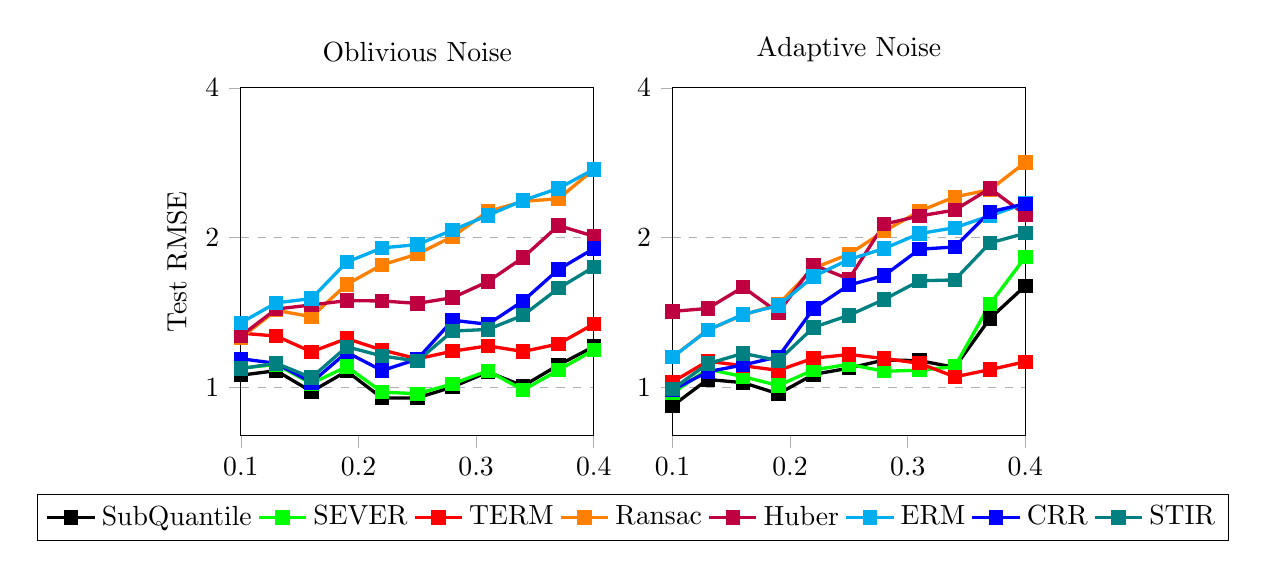
\begin{tikzpicture}
			\begin{groupplot}[group style={
					group name=myplot,
					group size= 2 by 1},height=6cm,width=0.5\linewidth,
				tick align=outside,
				tick pos=left,
				legend pos=outer north east,
				x grid style={darkgray176},
				xmin=0.1, xmax=0.4,
				xtick style={color=darkgray176},
				y grid style={darkgray176},
				ymin=0.8, ymax=4,
				ytick style={color=darkgray176},
				%ytick={0.1,1,6},
				ymajorgrids=true,
				grid style=dashed,
				ymode=log,
				log basis y={2},
				log ticks with fixed point,
				]
				\nextgroupplot[ylabel=Test RMSE,title=Oblivious Noise]
				\coordinate (c1) at (current axis.left of origin);
				\addplot [very thick, black,mark=square*]
				table {%
					0.1 1.05894804000854
					0.13 1.08117437362671
					0.16 0.981778621673584
					0.19 1.07855093479156
					0.22 0.952977478504181
					0.25 0.95321524143219
					0.28 1.00289475917816
					0.31 1.07451725006104
					0.34 1.00772738456726
					0.37 1.10959303379059
					0.4 1.20861554145813
				};
				\addplot [very thick, green,mark=square*]
				table {%
					0.1 1.09437942504883
					0.13 1.1125750541687
					0.16 1.01856243610382
					0.19 1.10203158855438
					0.22 0.979086935520172
					0.25 0.971916973590851
					0.28 1.01723539829254
					0.31 1.08105278015137
					0.34 0.988381624221802
					0.37 1.08411836624146
					0.4 1.18908596038818
				};
				\addplot [very thick, red,mark=square*]
				table {%
					0.1 1.28610801696777
					0.13 1.26911568641663
					0.16 1.17995369434357
					0.19 1.25433683395386
					0.22 1.1894918680191
					0.25 1.14218485355377
					0.28 1.18342161178589
					0.31 1.21262955665588
					0.34 1.18143332004547
					0.37 1.22365653514862
					0.4 1.34175312519073
				};
				\addplot [very thick, orange,mark=square*]
				table {%
					0.1 1.25890374183655
					0.13 1.42965865135193
					0.16 1.38786888122559
					0.19 1.61200165748596
					0.22 1.76458513736725
					0.25 1.85363411903381
					0.28 2.01117467880249
					0.31 2.25760555267334
					0.34 2.36710119247437
					0.37 2.39467430114746
					0.4 2.74260425567627
				};
				\addplot [very thick, purple,mark=square*]
				table {%
					0.1 1.27051901817322
					0.13 1.43797767162323
					0.16 1.46554577350616
					0.19 1.4952220916748
					0.22 1.49277687072754
					0.25 1.47613513469696
					0.28 1.51563453674316
					0.31 1.63231635093689
					0.34 1.82555913925171
					0.37 2.11563324928284
					0.4 2.01430583000183
				};
				\addplot [very thick, cyan,mark=square*]
				table {%
					0.1 1.34950256347656
					0.13 1.47964179515839
					0.16 1.50942897796631
					0.19 1.78661096096039
					0.22 1.90832722187042
					0.25 1.93754911422729
					0.28 2.07222437858582
					0.31 2.21759843826294
					0.34 2.37727379798889
					0.37 2.51313090324402
					0.4 2.7425274848938
				};
				\addplot [very thick, blue,mark=square*]
				table { 
					0.1 1.14254951477051
					0.13 1.11852920055389
					0.16 1.02382397651672
					0.19 1.17711758613586
					0.22 1.08173727989197
					0.25 1.14027178287506
					0.28 1.36521399021149
					0.31 1.34000027179718
					0.34 1.4935063123703
					0.37 1.72718107700348
					0.4 1.9017117023468
				};
				\addplot [very thick, teal,mark=square*]
				table { 
					0.1 1.0913804769516
					0.13 1.11872482299805
					0.16 1.04714918136597
					0.19 1.20770883560181
					0.22 1.15711236000061
					0.25 1.13065195083618
					0.28 1.2987471818924
					0.31 1.30847465991974
					0.34 1.3973708152771
					0.37 1.58278977870941
					0.4 1.74616122245789
				};
				\nextgroupplot[legend to name={DrugLegend},legend style={legend columns=8},title=Adaptive Noise]
				\coordinate (c2) at (current axis.right of origin);% I moved this to the upper right corner
				\addplot [very thick, black,mark=square*]
				table {%
					0.1 0.919014692306519
					0.13 1.03824925422668
					0.16 1.02291512489319
					0.19 0.97149395942688
					0.22 1.06282556056976
					0.25 1.09392309188843
					0.28 1.13588070869446
					0.31 1.13273966312408
					0.34 1.09808433055878
					0.37 1.37765526771545
					0.4 1.60075807571411
				};\addlegendentry{SubQuantile}
				\addplot [very thick, green,mark=square*]
				table {%
					0.1 0.97418487071991
					0.13 1.08860313892365
					0.16 1.05181241035461
					0.19 1.00930380821228
					0.22 1.08544754981995
					0.25 1.1134250164032
					0.28 1.07825410366058
					0.31 1.08377873897552
					0.34 1.10134482383728
					0.37 1.47154355049133
					0.4 1.8292989730835
				};\addlegendentry{SEVER}
				\addplot [very thick, red,mark=square*]
				table {%
					0.1 1.02624189853668
					0.13 1.12964737415314
					0.16 1.10623836517334
					0.19 1.08269572257996
					0.22 1.145876288414
					0.25 1.16499924659729
					0.28 1.14380311965942
					0.31 1.11899161338806
					0.34 1.05105876922607
					0.37 1.08660757541656
					0.4 1.12682223320007
				};\addlegendentry{TERM}
				\addplot [very thick, orange,mark=square*]
				table {%
					0.1 1.15098297595978
					0.13 1.3056538105011
					0.16 1.39799237251282
					0.19 1.47036576271057
					0.22 1.73723542690277
					0.25 1.85315310955048
					0.28 2.06100988388062
					0.31 2.26056098937988
					0.34 2.41652727127075
					0.37 2.49730658531189
					0.4 2.8336808681488
				};\addlegendentry{Ransac}
				\addplot [very thick, purple,mark=square*]
				table {%
					0.1 1.42236399650574
					0.13 1.44193506240845
					0.16 1.59146368503571
					0.19 1.41443765163422
					0.22 1.76296734809875
					0.25 1.65182590484619
					0.28 2.12984800338745
					0.31 2.21157455444336
					0.34 2.27279591560364
					0.37 2.51102018356323
					0.4 2.22447919845581
				};\addlegendentry{Huber}
				\addplot [very thick, cyan,mark=square*]
				table {%
					0.1 1.1504899263382
					0.13 1.30415141582489
					0.16 1.40286934375763
					0.19 1.46106946468353
					0.22 1.67240214347839
					0.25 1.80807554721832
					0.28 1.90281105041504
					0.31 2.0385856628418
					0.34 2.09466600418091
					0.37 2.21419143676758
					0.4 2.34415864944458
				};\addlegendentry{ERM}
				\addplot [very thick, blue,mark=square*]
				table { 
					0.1 0.988592743873596
					0.13 1.07592439651489
					0.16 1.11025428771973
					0.19 1.15290307998657
					0.22 1.44147706031799
					0.25 1.60702550411224
					0.28 1.67903292179108
					0.31 1.8964900970459
					0.34 1.91637253761292
					0.37 2.25444078445435
					0.4 2.34002900123596
				};\addlegendentry{CRR}
				\addplot [very thick, teal,mark=square*]
				table { 
					0.1 0.992274522781372
					0.13 1.11690032482147
					0.16 1.17126822471619
					0.19 1.13344883918762
					0.22 1.32121670246124
					0.25 1.39682495594025
					0.28 1.50348544120789
					0.31 1.638547539711
					0.34 1.64548587799072
					0.37 1.95285272598267
					0.4 2.04142189025879
				};\addlegendentry{STIR}
			\end{groupplot}
			\coordinate (c3) at ($(c1)!.5!(c2)$);
			\node[below] at (c3 |- current bounding box.south)
			{\pgfplotslegendfromname{DrugLegend}};
		\end{tikzpicture}
		\caption{\texttt{Drug Discovery} Dataset with Normal Noise and Structured Noise}
		\label{fig:drug-discovery}
	\end{figure}

	\begin{table}[!h]
		\centering
		\begin{tabular}{lcccc}
			\toprule 
			\textbf{Objectives}&\multicolumn{4}{c}{Test RMSE (\texttt{Drug Discovery})}\\                   
			\cmidrule(rl){2-5}
			&\subhead{$\eps = 0.1$}& \subhead{$\eps = 0.2$}& \subhead{$\eps = 0.3$}& \subhead{$\eps = 0.4$}\\ 
			\midrule
			ERM  &$1.303_{(0.0665)}$&$1.790_{(0.0849)}$&$2.198_{(0.0645)}$&$2.623_{(0.1010)}$\\
			CRR \cite{bhatia2017}  &$1.079_{(0.0899)}$&$1.125_{(0.0832)}$&$1.385_{(0.1372)}$&$1.725_{(0.1136)}$\\
			STIR \cite{pmlr-v89-mukhoty19a} &$1.087_{(0.1256)}$&$1.167_{(0.0750)}$&$1.403_{(0.0987)}$&$1.668_{(0.1142)}$\\
			Robust Risk \cite{RRM} &$1.176_{(0.1110)}
			$&$1.336_{(0.1882)}$&$1.437_{(0.1723)}$&$1.800_{(0.0820)}$\\
			SMART \cite{https://doi.org/10.48550/arxiv.2206.04777} &$1.094_{(0.1065)}$&$1.323_{(0.0758)}$&$1.578_{(0.0799)}$&$1.984_{(0.2020)}$\\
			TERM \cite{li2020tilted} &$\mathbf{1.029_{(0.0707)}}$&$1.126_{(0.0776)}$&$1.191_{(0.1091)}$&$1.201_{(0.1409)}$\\
			SEVER \cite{DiakonikolasKKLSS19} &$1.043_{(0.0970)}$&$\mathbf{1.067_{(0.0457)}}$&$\mathbf{1.071_{(0.0807)}}$&$\mathbf{1.138_{(0.1162)}}$\\
			Huber \cite{Huber2009} &$1.412_{(0.0474)}$&$1.501_{(0.2918)}$&$2.231_{(0.9054)}$&$2.247_{(1.0399)}$\\
			RANSAC \cite{RANSAC1981} &$1.238_{(0.0529)}$&$1.643_{(0.1331)}$&$2.092_{(0.1935)}$&$2.679_{(0.1365)}$\\
			\rowcolor{LightCyan}
			SubQuantile($p = 1-\eps$) &$\mathbf{0.966_{(0.1119)}}$&$\mathbf{1.002_{(0.1025)}}$&$\mathbf{1.010_{(0.0630)}}$&$\mathbf{1.082_{(0.1066)}}$\\
			\midrule 
			Genie ERM &$0.960_{(0.0845)}$&$0.982_{(0.0842)}$&$1.006_{(0.0879)}$&$1.030_{(0.0578)}$\\
			\bottomrule
		\end{tabular}
		\caption{\texttt{Drug Discovery} Dataset. Empirical Risk over $P$ with oblivious noise}
		\label{tab:drug-discovery}
	\end{table}
	
	As we can see in Table \ref{tab:drug-discovery}, we obtain state of the art results throughout all noise regimes. This makes our model the strongest among the tested, due to our strength throughout the whole range of noises. This dataset is also 
	
	\section{Conclusion}
	In this work we provide a theoretical analysis for robust linear regression by minimizing the \textit{Sub-Quantile} of the Empirical Risk. Furthermore, we run various numerical experiments and compare against the current State of the Art in Robust Linear Regression. Since minimizing over the subquantile is a general machine learning framework, it is scalable to larger scale machine learning problems. In future work, more real world applications can be explored and the theory can be expanded beyond linear regression. 
	
	\newpage

	\bibliographystyle{iclr2023_conference}
	\bibliography{iclr2023_conference}
	
	\begin{appendices}
		
	\newpage
	\appendix
	\startcontents[sections]
	\printcontents[sections]{l}{1}{\setcounter{tocdepth}{2}}
	\newpage
	
	\newgeometry{left=2cm,right=2cm,bottom=2cm}
	
	\section{Linear Algebra and Probability Theory Preliminaries}
	
	\begin{fact} The spectral norm of a matrix, $A$, an $(m \times n)$ matrix, is defined as follows
		\begin{equation}
			\norm{A}_2 = \sqrt{\lambda_{\max}\left(A^T A\right)} = \sigma_{\max}(A)
		\end{equation}
		It similarly follows:
		\begin{equation}
			\norm{A^T A}_2 = \norm{A}^2_2
		\end{equation}
	\end{fact}

	\begin{fact}
		\textbf{Weyl's Inequality} states the following:\\ If $M$, $N$, and $R$ are $n \times n$ Hermitian Matrices with the following eigenvalues where $M = N + R$:
		\begin{equation*}
			M: \mu_1 \geq \cdots \geq \mu_n
		\end{equation*}
		\begin{equation*}
			N: \nu_1 \geq \cdots \geq \nu_n
		\end{equation*}
		\begin{equation*}
			R: \rho_1 \geq \cdots \geq \rho_n
		\end{equation*}
		Then the following equalities hold:
		\begin{equation*}
			\nu_i + \rho_n \leq \mu_i \leq \nu_i + \rho_1 \text { for } i = 1,\dots,n
		\end{equation*}
	\end{fact}

	\begin{fact}
		Let $A$ be a $n \times m$ matrix with $n \gg m$. It then follows:
		\begin{equation}
			A^T A = \left(U \Sigma V^T\right)^T \left(U \Sigma V^T \right) = \left(V\Sigma^T U^T\right)\left(U \Sigma V^T\right) = V \Sigma^T \Sigma V^T = V D V^T
		\end{equation}
		where $D = \Sigma^T \Sigma = \begin{pmatrix} \sigma_1^2 & & & \\ & \sigma_2^2 & & \\ & & \ddots & \\ & & & \sigma_m^2 \end{pmatrix}$
	\end{fact}

	\begin{fact}
		This is a restatement from \cite{Wackerly2008}.\\
		Let $X_1,\cdots, X_n$ be i.i.d continuous random variables with common distribution function $F(y)$ and common probability density function $f(x)$. If $X_{(k)}$ denotes the $k$th-order statistic, then the density function of $X_{(k)}$ is given by:
		\begin{equation}
			g_{(k)}(x_k) = \frac{n!}{(k-1)!(n-k)!}[F(x_k)]^{k-1}[1 - F(x_k)]^{n-k}f(x_k)
		\end{equation}
	\end{fact}

	\begin{fact}
		The cdf of the $k$th order statistic from a sample of $n$ is:
		\begin{equation}
			F_{(k,n)} = \mathbb{P}\left[X_{(k)}\leq x \right] = \sum_{j=k}^n \begin{pmatrix} n \\ j\end{pmatrix} \left(1 - F(x)\right)^{n-j} F(x)^j
		\end{equation}
	\end{fact}

	\newpage
	
	\section{Theory for Ridge Regression Algorithm \ref{alg:sqo-ridge}}\label{app:sub-quantile-optimization}
	\subsection{Proof of Theorem~\ref{thm:expected-value-corrupted}}\label{app:expected-value-corrupted}
	\begin{proof}
	\begin{assumption}\label{asm:normal-sampling}
		The rows of $P$ and $Q$ are sampled from $\vzero$ centered Normal Distributions.
		\begin{equation*}
			P_i \sim \mathcal{N}\left(\vzero, \Sigma_P\right)
		\end{equation*}
		\begin{equation}
			Q_i \sim \mathcal{N}\left(\vzero, \Sigma_Q\right)
		\end{equation}
	\end{assumption}
	
	\begin{assumption}\label{asm:wishart}
		By assumption \ref{asm:normal-sampling}, it thus follows that the matrices $P^T P$ and $Q^T Q$ are sampled from Wishart Distributions.
		\begin{equation}
			P^T P \sim \mathcal{W}\left(n,\Sigma_P\right)
		\end{equation}
		\begin{equation}
			Q^T Q \sim \mathcal{W}\left(n, \Sigma_Q\right)
		\end{equation}
	\end{assumption}

	\begin{assumption}\label{asm:identity-covariance}
		Similar to the assumption made in \cite{bhatia2017}, to give theoretical bounds on the our algorithm, we assume the following:
		\begin{equation}
			\Sigma_P = \xi_P I
		\end{equation}
		\begin{equation} 
			\Sigma_Q = \xi_Q I
		\end{equation}
		where $\xi_P,\xi_Q \geq 0$ 
	\end{assumption}
	The closed form solution for Ridge Regression with regularization parameter $\lambda$ is equal to the following:
	\begin{equation}
		\hat{\vbeta} = \left(X^T X+ \lambda I\right)^{-1}X^T y
	\end{equation}
	We will use this to bound the difference of the $\vbeta_P$ and $\vtheta_{(k)}$.
	\begin{align*}
		\norm{\vbeta_P - \vtheta_{(k)}}_2 &= \norm{\vbeta_P - \left(S^T S + \lambda I\right)^{-1}S^T \vy}_2 &&\\
	\end{align*}
	Note the subquantile matrix $S$, consists of data points from $P$ and $Q$, we will reorganize $S$ into the following:
	\begin{equation*}
		S = \begin{pmatrix}P \\ Q \end{pmatrix} = 
		\begin{pmatrix}
			\leftarrow & \vp_1 & \rightarrow \\
			\vdots & \vdots & \vdots \\
			\leftarrow & \vp_{n(1-\varepsilon^{(t)})} & \rightarrow\\
			\leftarrow & \vq_1 & \rightarrow \\
			\vdots & \vdots & \vdots \\
			\leftarrow & \vq_{n\varepsilon^{(t)}} & \rightarrow
		\end{pmatrix}\text{ and } \vy = \begin{pmatrix}\vy_P \\ \vy_Q \end{pmatrix} = \begin{pmatrix} \vbeta_P\vp_1 + \eps_P \\ \vdots \\ \vbeta_P\vp_{(n(1-\varepsilon^{(t)}))} + \eps_P \\ \vbeta_Q\vq_1 + \eps_Q\\ \vdots \\ \vbeta_Q\vq_{n\varepsilon^{(t)}} + \eps_Q\end{pmatrix}
	\end{equation*}
	Let us also assume $\Var(\eps_P) = \eta_P$ and $\Var(\eps_Q) = \eta_Q$. Then we can make the following manipulations:
	\begin{align*}
		= &\norm{\vbeta_P - \left(P^T P + Q^T Q + \lambda I\right)^{-1}\begin{pmatrix}P^T Q^T\end{pmatrix}\begin{pmatrix}\vy_P \\ \vy_Q \end{pmatrix}}_2 &&\\
		= &\norm{\left(P^T P + \lambda I\right)^{-1} P^T \vy_P - \left(P^T P + Q^T Q + \lambda I\right)^{-1}P^T \vy_P  - \left(P^T P + Q^T Q + \lambda I\right)^{-1}Q^T \vy_Q}_2 &&\\
		\leq &\norm{\left(P^T P + \lambda I\right)^{-1} P^T \vy_P -\left(P^T P + Q^T Q+ \lambda I\right)^{-1}P^T \vy_P}_2 + \norm{\left(P^T P + Q^T Q+ \lambda I\right)^{-1}Q^T \vy_Q}_2 &&\\
		\leq& \norm{\left(P^T P + \lambda I\right)^{-1}}_2 \norm{P^T\vy_P}_2 + \norm{\left(P^T P + Q^T Q + \lambda I\right)^{-1}}_2\norm{P^T \vy_P}_2 + \norm{\left(P^T P + Q^T Q + \lambda I\right)^{-1}}_2\norm{Q^T \vy_Q}_2&&\\
		\leq & \sqrt{\lambda_{\max}\left(P^T P\right)}\left(\norm{\left(P^TP + \lambda I\right)^{-1}}_2+\norm{\left(P^T P + Q^T Q + \lambda I\right)^{-1}}_2\right)\norm{\vy_P}_2 + \sqrt{\lambda_{\max}\left(Q^T Q\right)}\norm{\left(P^T P + Q^T Q + \lambda I\right)^{-1}}_2\norm{\vy_Q}_2 &&\\
		= &\frac{\sigma_{\max}(P)\norm{\vy_P}}{\sqrt{\lambda_{\max}(P^TP + \lambda I)}} + \frac{\sigma_{\max}(P)\norm{\vy_P}_2}{\sqrt{\lambda_{\max}\left(P^T P + Q^T Q + \lambda I\right)}} + \frac{\sigma_{\max}(Q)\norm{\vy_Q}_2}{\sqrt{\lambda_{\max}\left(P^T P + Q^T Q + \lambda I\right)}} &&\\
		\overset{\mathrm{(a)}}{\leq} &\frac{2\sigma_{\max}(P)\norm{P\vbeta_P + \veps_P}_2 + \sigma_{\max}{Q}\norm{Q\vbeta_Q + \veps_Q}_2}{\sqrt{\lambda_{\max}\left(P^T P + \lambda I\right)}} &&\\
		\overset{\mathrm{(b)}}{\leq} & \frac{2\sigma^2_{\max}(P)\norm{\vbeta_P} + 6\sigma_{\max}(P)n(1-\varepsilon^{(t)})\eta_P + \sigma^2_{\max}(Q)\norm{\vbeta_Q} + 3\sigma_{\max}(Q)n\varepsilon^{(t)}\eta_Q}{\sqrt{\lambda_{\max}(P^T P) + \lambda_{\min}(\lambda I)}} &&\\
		\leq &\frac{2\sigma^2_{\max}(P)\norm{\vbeta_P} + 6\sigma_{\max}(P)n(1-\varepsilon^{(t)})\eta_P + \sigma^2_{\max}(Q)\norm{\vbeta_Q} + 3\sigma_{\max}(Q)n\varepsilon^{(t)}\eta_Q}{\sqrt{\sigma^2_{\max}(P) + \lambda}} &&\\
	\end{align*}
	
	(a) is due to $Q^TQ$ being a positive semi definite symmetric matrix. \\ 
	(b) holds with high probability due to the variance of the $\chi^2$ distribution\\
	
	Thus we have shown that $\norm{\vbeta_P - \vtheta_{(t)}}_2$ is bounded above at any time-step $(t)$ in terms of the maximal singular values of the data matrices and the variance of the white noise. 
	
	\end{proof}

	\newpage
	
	\section{Proofs for $\varepsilon^{(t)}$}
	Let us note the Subquantile Matrix $\displaystyle S = \begin{pmatrix} P \\ Q \end{pmatrix} = \begin{pmatrix} \leftarrow & \vp_1 & \rightarrow \\ \vdots & \vdots & \vdots \\ \leftarrow & \vp_{\eta_P} & \rightarrow \\ \leftarrow & \vq_1 & \rightarrow \\ \vdots & \vdots & \vdots \\ \leftarrow & \vq_{\eta_Q} & \rightarrow\end{pmatrix}$. Thus we can define: $\displaystyle \varepsilon^{(t)} = \frac{\eta_Q}{\eta_P + \eta_Q} = \frac{\eta_Q}{np}$. Where $n$ is the number of training examples and $p$ is the Subquantile we are minimizing over. In this section, we want to provide a theoretical upper bound on $\eta_Q$, from where we can upper bound $\varepsilon^{(t)}$ which is stronger than the trivial upper bound of $\displaystyle \frac{\epsilon}{p}$. We will approach this problem with Order Statistics.
	\begin{assumption}
		The optimal regressors are linearly independent, i.e. $\vbeta_P \neq \gamma \vbeta_Q\, \forall \gamma \in \mathbb{R}$
	\end{assumption}
	Let $\displaystyle \vtheta_{(t)} = \alpha_1 \vbeta_P + \alpha_2 \vbeta_Q + \sum_{i=3}^{d}\vr_i$.
	
	Let us denote $P_1 < P_2 < \dots < P_{n(1 - \epsilon)}$ as the order statistics of the random variable $P \sim \left(\vp_i \vtheta - (\vp_i \vbeta_P + \epsilon_P)\right)^2$ where $ \vp_i \sim \mathcal{N}_d(\vzero, \xi_P I)$. Let us also denote $Q_1 < Q_2 < \dots < Q_{n(1 - \epsilon)}$ as the order statistics of the random variable $Q \sim \left(\vq_i \vtheta - (\vp_i \vbeta_Q + \epsilon_Q)\right)^2$ where $ \vq_i \sim \mathcal{N}_d(\vzero, \xi_P I)$.\\
	First we will formalize the CDF of $P$ and $Q$. Note $\vp_i$ and $\vq_i$ represent the normally sampled gaussian data. 
	\begin{align}
		P_i = &\left(\vp_i\vtheta_{(t)} - (\vp_i \vbeta_P + \eps_P)\right)^2 &&\\
		 = &\left(\vp_i(\vtheta_{(t)} - \vbeta_P) - \eps_P\right)^2 &&\\
		= &\left(\vp_i(\vtheta_{(t)} - \vbeta_P)\right)^2 - 2 \eps_P \left(\vp_i(\vtheta_{(t)} - \vbeta_P)\right) + \eps_P^2 &&
	\end{align}
	As $\mathbb{E}\left[\epsilon_P\right] = 0$, we will only consider the case $\epsilon_P = 0$. This simplifies $P_i$ and $Q_i$:
	\begin{equation}
		P_i = \left(\mP_i(\vtheta_{(t)} - \vbeta_P)\right)^2 
	\end{equation}
	\begin{equation}
		Q_i = \left(\mQ_i(\vtheta_{(t)} - \vbeta_Q)\right)^2
	\end{equation}
	Let us note all the entries of $\mP_i$ are sampled from $\mathcal{N}(0,\xi_P)$ and all entries of $\mQ_i$ are sampled from $\mathcal{N}(0,\xi_Q)$.
	It thus follows:
	\begin{align*}
		\left(\mP_i(\vtheta_{(t)} - \vbeta_P)\right)^2 &= \left(\sum_{j=1}^d\mathcal{N}(0,\xi_P)\left(\theta^{(t)}_j - \beta_{Pj}\right)\right)^2 &&\\
		&= \left(\sum_{j=1}^d \mathcal{N}\left(0,\xi_P\left(\theta_j^{(t)} - \beta_{Pj}\right)^2\right)\right)^2  &&\\
		&= \left(\mathcal{N}\left(0, \sum_{j=1}^d \xi_P\left(\theta_j^{(t)} - \beta_{Pj}\right)^2\right)\right)^2
	\end{align*}
	It thus similarly follows for $Q_i$:
	\begin{equation*}
		\left(\mQ_i(\vtheta_{(t)} - \vbeta_Q)\right)^2 = \left(\mathcal{N}\left(0, \sum_{j=1}^d \xi_Q\left(\theta_j^{(t)} - \beta_{Qj}\right)^2\right)\right)^2
	\end{equation*}
	Now we can define the cumulative distribution functions.
	\begin{align}
		F_P(z) &= \frac{1}{\sqrt{2\pi}}\int_{-\sqrt{z}}^{\sqrt{z}}\exp\left(-\frac{u^2}{2\sum_{j=1}^d \xi_P\left(\theta_j^{(t)} - \beta_{Pj}\right)^2}\right)du &&\\
		&= \Phi\left(\frac{\sqrt{z}}{\sqrt{\sum_{j=1}^d \xi_P\left(\theta_j^{(t)}-\beta_{Pj}\right)^2}}\right) - \Phi\left(\frac{-\sqrt{z}}{\sqrt{\sum_{j=1}^d \xi_Q\left(\theta_j^{(t)}-\beta_{Pj}\right)^2}}\right) &&
	\end{align}
	Let us define $\displaystyle \phi = \sum_{j=1}^d \xi_P\left(\theta_j^{(t)} - \beta_{Pj}\right)^2$ and $\displaystyle \psi = \sum_{j=1}^d \xi_Q\left(\theta_j^{(t)} - \beta_{Qj}\right)^2$
	Therefore it follows:
	\begin{equation}
		F_P(z) = \Phi\left(\frac{\sqrt{z}}{\sqrt{\phi}}\right) - \Phi\left(\frac{-\sqrt{z}}{\sqrt{\phi}}\right)
	\end{equation}
	Similarly for $F_Q(z)$ it follows:
	\begin{equation}
		F_Q(z) = \Phi\left(\frac{\sqrt{z}}{\sqrt{\psi}}\right) - \Phi\left(\frac{-\sqrt{z}}{\sqrt{\psi}}\right)
	\end{equation}
	Here we can note if $\phi < \psi$, then for all $z > 0$, it follows $F_P(z) > F_Q(z)$.
	
	We now want to find the max integer, $\eta$ such that with probability greater than $0.9$, $Q_{\eta} < P_{np - \eta}$ and for all $m \in \mathbb{N}$ such that $m > \eta$, $Q_{m} > P_{np - \eta}$. This is equivalent to the probability there will be $\eta$ elements from $Q$ within the Subquantile matrix.

	\begin{align*}
		\mathbb{P}\left[Q_\eta < P_{np - \eta} \bigcap_{i=1}^{n\epsilon - \eta} Q_{\eta+ i} > P_{np - \eta}\right] &= \mathbb{P}\left[Q_\eta < P_{np - \eta}\right] \prod_{i=1}^{n\epsilon - \eta} \mathbb{P}\left[Q_{n+i} > P_{np - \eta}\right] &&\\
		&= \mathbb{P}\left[Q_n < P_{np - \eta}\right]\prod_{i=1}^{n\epsilon - \eta}\left(1 - \mathbb{P}\left[Q_{n+i} < P_{np - \eta}\right]\right) &&\\
		&= \mathbb{P}\left[Q_n - P_{np-\eta} < 0\right]\prod_{i=1}^{n\epsilon - \eta} \left(1 - \mathbb{P}\left[Q_{n+i} - P_{np-\eta} < 0\right]\right) &&\\
	\end{align*}
	It follows $\eta$ will be lower depending on the difference of $\phi$ and $\psi$. In a further work we will give a tight upper bound on the probability.

	
	\newpage
	\section{Theory for Subquantile Minimization}\label{app:general-proofs}
	\subsection{Derivation of Lemma~\ref{lem:gfermat}}
	\label{app:gfermat}
	Since $\displaystyle g(t,\vtheta)$ is a concave function. Maximizing $g(t,\vtheta)$ is equivalent to minimizing $-g(t,\vtheta)$. We will find fermat's optimality condition for the function $\displaystyle -g(t,\vtheta)$, which is convex. 
	Let $\displaystyle \hat{\vnu} = sorted\left((\vtheta^T X - y)^2\right)$ and note $\displaystyle 0 < p < 1$
	\begin{align}
		\partial{\displaystyle (-g(t,\boldsymbol{\theta}})) &= \partial{\left(-t + \frac{1}{np}\sum_{i=1}^{n}(t-\hat{\vnu}_i)^+\right)} &&\\
		&= \partial{(-t)} + \partial{\left(\frac{1}{np}\sum_{i=1}^{n}(t-\hat{\vnu}_i)^+\right)}&&\\
		&= -1 + \frac{1}{np}\sum_{i=1}^{n}\partial{(t-\hat{\vnu}_i)^+} &&\\
		&= -1 + \frac{1}{np}\sum_{i=1}^{n}
		\left\{
		\begin{array}{lr}
			1, & \text{if } t > \hat{\vnu}_i\\
			0, & \text{if } t < \hat{\vnu}_i \\
			\left[0,1\right], & \text{if } t = \hat{\vnu}_i \\
		\end{array}
		\right\}&&\\
		&= 0 \text{ when }\displaystyle t = \hat{\vnu}_{np}&&
	\end{align}
	This is the $p$-quantile of $\displaystyle \vnu$. Assuming no two points are equal in the dataset, this means the minimizing value for $t$ has a range of values, $\hat{\vnu}_{np} \leq t < \hat{\vnu}_{np+1}$. This means $g(t,\vtheta)$ is not strongly convex with respect to $t$. 
	\subsection{Derivation of Lemma~\ref{lem:gthetaderiv}}
	\label{app:gthetaderiv}
		Note that $t_k = \vnu_{np}$ which is equivalent to $(\vtheta_k^T\vx_{np} - y_{np})^2$
		\begin{align*}
			\nabla_{\vtheta_k} g(t_{k+1},\vtheta_k) &= \nabla_{\vtheta_k}\left(\vnu_{np} - \frac{1}{np}\sum_{i=1}^n(\vnu_{np} - (\vtheta_k^T\vx_i - y_i)^2)^+\right) &&\\
			&= \nabla_{\vtheta_k}\left((\vtheta_k^T\vx_{np}-y_{np})^2 - \frac{1}{np}\sum_{i=1}^n\left((\vtheta_k^T\vx_{np} - y_{np})^2 - (\vtheta_k^T\vx_i - y_i)^2\right)^+\right) &&\\
			&= \nabla_{\vtheta_k}(\vtheta_k^T\vx_{np}-y_{np})^2 - \frac{1}{np}\sum_{i=1}^n\nabla_{\vtheta_k}\left((\vtheta_k^T\vx_{np} - y_{np})^2 - (\vtheta_k^T\vx_i - y_i)^2\right)^+ &&\\				
			&= 2\vx_{np}(\vtheta_k^T\vx_{np} - y_{np}) -\frac{1}{np}\sum_{i=1}^{n}2\vx_{np}(\vtheta_k^T\vx_{np} - y_{np}) \notag\\ &\qquad-2\vx_i(\vtheta_k^T\vx_i - y_i) \left\{
			\begin{array}{lr}
				1, & \text{if } t > v_i\\
				0, & \text{if } t < v_i \\
				\left[0,1\right], & \text{if } t = v_i \\
			\end{array} \right\} &&\\
			&= 2\vx_{np}(\vtheta_k^T\vx_{np} - y_{np}) -\frac{1}{np}\sum_{i=1}^{np}2\vx_{np}(\vtheta_k^T\vx_{np} - y_{np}) -2\vx_i(\vtheta_k^T\vx_i - y_i) &&\\	
			&= 2\vx_{np}(\vtheta_k^T\vx_{np} - y_{np}) - 2\vx_{np}(\vtheta_k^T\vx_{np} - y_{np}) + \frac{1}{np}\sum_{i=1}^{np}2\vx_i(\vtheta_k^T\vx_i - y_i) &&\\
			&= \frac{1}{np}\sum_{i=1}^{np}2\vx_i(\vtheta_k^T\vx_i - y_i)&&
		\end{align*}
		This is the derivative of the $np$ samples with lowest error with respect to $\vtheta$.

	\subsection{Derivation of Lemma~\ref{lem:g-lsmooth}}
	The objective function 
	$\displaystyle g(\vtheta,t)$ is $L$-smooth w.r.t $\vtheta$ iff
	\begin{equation}
		||  \nabla_\vtheta g(\vtheta',t) - \nabla_\vtheta g(\vtheta,t) || \leq L|| \vtheta' - \vtheta || 
	\end{equation}
	\begin{align}
		\norm{ \nabla_{\vtheta} g(\vtheta^{'},t) - \nabla_{\vtheta} g(\vtheta,t) } = &\norm{ \frac{1}{np}\sum_{i=1}^{np}2\vx_i(\vtheta_k^{'\top} \vx_i - y_i) - \frac{1}{np}\sum_{i=1}^{np}2\vx_i(\vtheta_k^T \vx_i - y_i) } &&\\
		= &\norm{\frac{1}{np}\sum_{i=1}^{np}2\vx_i(\vtheta_k^{'\top}\vx_i - \vtheta_k^T\vx_i)}&&\\
		= &\norm{\frac{1}{np}\sum_{i=1}^{np}2\vx_i\vx_i^T(\vtheta_k^{'\top} - \vtheta_k^T)} &&\\
		\overset{\mathrm{Cauchy-Schwarz}}{\leq} &\norm{\frac{2}{np}\sum_{i=1}^{np}\vx_i\vx_i^T}\norm{\vtheta_k^{'\top} - \vtheta_k^T} &&\\
		= &L\norm{\vtheta_k^{'\top} - \vtheta_k^T} &&
	\end{align}
	where $\displaystyle L = \norm{\frac{2}{np}X^T X}$\\
	This concludes the derivation.
	\subsection{Proof of Lemma~\ref{lem:g-change-wrt-t}}
	\label{app:g-change-wrt-t}
	\begin{proof}
		We will investigate the two cases $t_{k+1} \leq t$ and $t_{k+1} > t_k$.\\
		\textbf{Case (i)} $t_{k+1} \leq t_k$\\
		Let us first expand out $g(t_k,\vtheta_k)$ with the knowledge that $t_k \geq \hat{\vnu_{k}}$
		\begin{align}
			g(t_k, \vtheta_k) &= t_k - \frac{1}{np}\sum_{i=1}^{n}(t_k-\vnu_i)^+ &&\\
			&= t_k - \frac{1}{np}(np)t_k + \frac{1}{np}\sum_{i=1}^{np}\vnu_i + \frac{1}{np}\sum_{i=np}^{n}(t_k - \vnu_i)^+ &&\\
			&= \frac{1}{np}\sum_{i=1}^{np}\vnu_i + \frac{1}{np}\sum_{i=np}^{n}(t_k - \vnu_i)^+ &&\\
			g(t_{k+1},\vtheta_k) - g(t_k,\vtheta_k) &=  \frac{1}{np}\sum_{i=1}^{np}\vnu_i - \left(\frac{1}{np}\sum_{i=1}^{np}\vnu_i + \frac{1}{np}\sum_{i=np}^{n}(t_k - \vnu_i)^+\right) &&\\
			&= - \frac{1}{np}\sum_{i=np}^{n}(t_k - \vnu_i)^+ &&
		\end{align}
		\textbf{Case (ii)} $t_{k+1} > t_k$\\
		Since we know $t_k$ is less than $\vnu_{np}$, WLOG we will say $t_k$ is greater than the lowest $n(p-\delta)$ elements, where $\delta \in (0,p)$. 
		\begin{align}
			g(t_k,\vtheta_k) &= t_k - \frac{1}{np}\sum_{i=1}^n(t_k - \vnu_i)^+ &&\\
			&= t_k - \frac{1}{np}\sum_{i=1}^{n(p-\delta)}(t_k - \vnu_i)^+ &&\\
			&= t_k - \frac{1}{np}(n(p-\delta))t_k + \frac{1}{np}\sum_{i=1}^{n(p-\delta)}\vnu_i &&\\
			g(t_k,\vtheta_{k+1}) - g(t_k,\vtheta_k) &= \frac{1}{np}\sum_{i=1}^{np}\vnu_i - \left(\delta t_k + \frac{1}{np}\sum_{i=1}^{n(p-\delta)}\vnu_i\right) &&\\
			&= \left(\frac{1}{np}\sum_{i=n(p-\delta)}^n\vnu_i\right) - \delta t_k &&
		\end{align}
		This concludes the proof.
	\end{proof}
  	
  	\newpage
	\section{Theory for Adaptive Linear Corruption}
	In this section, we provide rigorous theory for why Sub-Quantile Minimization works so well in the case of corruption of the form $\displaystyle \vbeta_Q^T \vmu = y_p + \eps_Q$.
	\begin{assumption}\label{asm:normal-error}
		The residuals of $\vtheta_k$ are normally distributed with respect to $\mathbb{P}$ and $\mathbb{Q}$. In other words, $\vtheta_k^T \vp - \vy_P$ and $\vtheta_k^T \vq - \vy_Q$ are normally distributed.
	\end{assumption}
	Assumption \ref{asm:normal-error} can be visually verified in figure \ref{fig:normal-residual}. Even after multiple iteration steps the residuals with respect to $\mathbb{P}$ and $\mathbb{Q}$ are still normal. Thus it follows by decreasing $\norm{\vtheta - \vbeta_P}_1$ more relative to $\norm{\vtheta - \vbeta_Q}_1$ then the SubQuantile will contain more points from $P$ by expectation. 
	\begin{figure}
		\begin{minipage}[htbp]{0.24\textwidth}
			\centering
			% This file was created with tikzplotlib v0.10.1.
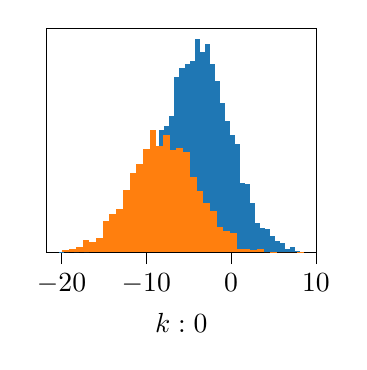
\begin{tikzpicture}

\definecolor{darkgray176}{RGB}{176,176,176}
\definecolor{darkorange25512714}{RGB}{255,127,14}
\definecolor{steelblue31119180}{RGB}{31,119,180}

\begin{axis}[
tick align=outside,
tick pos=left,
x grid style={darkgray176},
xlabel={$k: 0$},
xmin=-21.7817629577121, xmax=10.0412651951797,
xtick style={color=black},
y grid style={darkgray176},
%ylabel={Frequency},
ymin=0, ymax=369.6,
%ytick style={color=black},
ytick=\empty,
scale=0.5
]
\draw[draw=none,fill=steelblue31119180] (axis cs:-20.3352616780352,0) rectangle (axis cs:-19.7415116521512,1);
\draw[draw=none,fill=steelblue31119180] (axis cs:-19.7415116521512,0) rectangle (axis cs:-19.1477616262672,0);
\draw[draw=none,fill=steelblue31119180] (axis cs:-19.1477616262672,0) rectangle (axis cs:-18.5540116003831,3);
\draw[draw=none,fill=steelblue31119180] (axis cs:-18.5540116003831,0) rectangle (axis cs:-17.9602615744991,0);
\draw[draw=none,fill=steelblue31119180] (axis cs:-17.9602615744991,0) rectangle (axis cs:-17.3665115486151,2);
\draw[draw=none,fill=steelblue31119180] (axis cs:-17.3665115486151,0) rectangle (axis cs:-16.7727615227311,0);
\draw[draw=none,fill=steelblue31119180] (axis cs:-16.7727615227311,0) rectangle (axis cs:-16.179011496847,4);
\draw[draw=none,fill=steelblue31119180] (axis cs:-16.1790114968471,0) rectangle (axis cs:-15.585261470963,3);
\draw[draw=none,fill=steelblue31119180] (axis cs:-15.585261470963,0) rectangle (axis cs:-14.991511445079,6);
\draw[draw=none,fill=steelblue31119180] (axis cs:-14.991511445079,0) rectangle (axis cs:-14.397761419195,13);
\draw[draw=none,fill=steelblue31119180] (axis cs:-14.397761419195,0) rectangle (axis cs:-13.804011393311,17);
\draw[draw=none,fill=steelblue31119180] (axis cs:-13.804011393311,0) rectangle (axis cs:-13.2102613674269,18);
\draw[draw=none,fill=steelblue31119180] (axis cs:-13.2102613674269,0) rectangle (axis cs:-12.6165113415429,30);
\draw[draw=none,fill=steelblue31119180] (axis cs:-12.6165113415429,0) rectangle (axis cs:-12.0227613156589,43);
\draw[draw=none,fill=steelblue31119180] (axis cs:-12.0227613156589,0) rectangle (axis cs:-11.4290112897749,55);
\draw[draw=none,fill=steelblue31119180] (axis cs:-11.4290112897749,0) rectangle (axis cs:-10.8352612638908,70);
\draw[draw=none,fill=steelblue31119180] (axis cs:-10.8352612638908,0) rectangle (axis cs:-10.2415112380068,102);
\draw[draw=none,fill=steelblue31119180] (axis cs:-10.2415112380068,0) rectangle (axis cs:-9.64776121212279,111);
\draw[draw=none,fill=steelblue31119180] (axis cs:-9.64776121212279,0) rectangle (axis cs:-9.05401118623877,140);
\draw[draw=none,fill=steelblue31119180] (axis cs:-9.05401118623877,0) rectangle (axis cs:-8.46026116035475,161);
\draw[draw=none,fill=steelblue31119180] (axis cs:-8.46026116035475,0) rectangle (axis cs:-7.86651113447072,201);
\draw[draw=none,fill=steelblue31119180] (axis cs:-7.86651113447072,0) rectangle (axis cs:-7.2727611085867,209);
\draw[draw=none,fill=steelblue31119180] (axis cs:-7.2727611085867,0) rectangle (axis cs:-6.67901108270267,225);
\draw[draw=none,fill=steelblue31119180] (axis cs:-6.67901108270267,0) rectangle (axis cs:-6.08526105681865,290);
\draw[draw=none,fill=steelblue31119180] (axis cs:-6.08526105681865,0) rectangle (axis cs:-5.49151103093463,304);
\draw[draw=none,fill=steelblue31119180] (axis cs:-5.49151103093463,0) rectangle (axis cs:-4.8977610050506,311);
\draw[draw=none,fill=steelblue31119180] (axis cs:-4.8977610050506,0) rectangle (axis cs:-4.30401097916658,315);
\draw[draw=none,fill=steelblue31119180] (axis cs:-4.30401097916658,0) rectangle (axis cs:-3.71026095328256,352);
\draw[draw=none,fill=steelblue31119180] (axis cs:-3.71026095328256,0) rectangle (axis cs:-3.11651092739853,330);
\draw[draw=none,fill=steelblue31119180] (axis cs:-3.11651092739853,0) rectangle (axis cs:-2.52276090151451,343);
\draw[draw=none,fill=steelblue31119180] (axis cs:-2.52276090151451,0) rectangle (axis cs:-1.92901087563049,310);
\draw[draw=none,fill=steelblue31119180] (axis cs:-1.92901087563049,0) rectangle (axis cs:-1.33526084974646,282);
\draw[draw=none,fill=steelblue31119180] (axis cs:-1.33526084974646,0) rectangle (axis cs:-0.741510823862438,247);
\draw[draw=none,fill=steelblue31119180] (axis cs:-0.741510823862438,0) rectangle (axis cs:-0.147760797978414,217);
\draw[draw=none,fill=steelblue31119180] (axis cs:-0.147760797978414,0) rectangle (axis cs:0.44598922790561,193);
\draw[draw=none,fill=steelblue31119180] (axis cs:0.44598922790561,0) rectangle (axis cs:1.03973925378963,179);
\draw[draw=none,fill=steelblue31119180] (axis cs:1.03973925378963,0) rectangle (axis cs:1.63348927967366,114);
\draw[draw=none,fill=steelblue31119180] (axis cs:1.63348927967366,0) rectangle (axis cs:2.22723930555768,112);
\draw[draw=none,fill=steelblue31119180] (axis cs:2.22723930555768,0) rectangle (axis cs:2.82098933144171,81);
\draw[draw=none,fill=steelblue31119180] (axis cs:2.82098933144171,0) rectangle (axis cs:3.41473935732573,49);
\draw[draw=none,fill=steelblue31119180] (axis cs:3.41473935732573,0) rectangle (axis cs:4.00848938320975,41);
\draw[draw=none,fill=steelblue31119180] (axis cs:4.00848938320975,0) rectangle (axis cs:4.60223940909378,38);
\draw[draw=none,fill=steelblue31119180] (axis cs:4.60223940909378,0) rectangle (axis cs:5.1959894349778,27);
\draw[draw=none,fill=steelblue31119180] (axis cs:5.1959894349778,0) rectangle (axis cs:5.78973946086182,18);
\draw[draw=none,fill=steelblue31119180] (axis cs:5.78973946086182,0) rectangle (axis cs:6.38348948674585,15);
\draw[draw=none,fill=steelblue31119180] (axis cs:6.38348948674585,0) rectangle (axis cs:6.97723951262987,6);
\draw[draw=none,fill=steelblue31119180] (axis cs:6.97723951262987,0) rectangle (axis cs:7.5709895385139,9);
\draw[draw=none,fill=steelblue31119180] (axis cs:7.5709895385139,0) rectangle (axis cs:8.16473956439792,3);
\draw[draw=none,fill=darkorange25512714] (axis cs:-19.8926246009193,0) rectangle (axis cs:-19.1013082532409,4);
\draw[draw=none,fill=darkorange25512714] (axis cs:-19.1013082532409,0) rectangle (axis cs:-18.3099919055625,6);
\draw[draw=none,fill=darkorange25512714] (axis cs:-18.3099919055625,0) rectangle (axis cs:-17.5186755578841,9);
\draw[draw=none,fill=darkorange25512714] (axis cs:-17.5186755578841,0) rectangle (axis cs:-16.7273592102057,20);
\draw[draw=none,fill=darkorange25512714] (axis cs:-16.7273592102057,0) rectangle (axis cs:-15.9360428625273,17);
\draw[draw=none,fill=darkorange25512714] (axis cs:-15.9360428625273,0) rectangle (axis cs:-15.1447265148489,23);
\draw[draw=none,fill=darkorange25512714] (axis cs:-15.1447265148489,0) rectangle (axis cs:-14.3534101671705,51);
\draw[draw=none,fill=darkorange25512714] (axis cs:-14.3534101671705,0) rectangle (axis cs:-13.5620938194922,63);
\draw[draw=none,fill=darkorange25512714] (axis cs:-13.5620938194922,0) rectangle (axis cs:-12.7707774718138,72);
\draw[draw=none,fill=darkorange25512714] (axis cs:-12.7707774718138,0) rectangle (axis cs:-11.9794611241354,103);
\draw[draw=none,fill=darkorange25512714] (axis cs:-11.9794611241354,0) rectangle (axis cs:-11.188144776457,131);
\draw[draw=none,fill=darkorange25512714] (axis cs:-11.188144776457,0) rectangle (axis cs:-10.3968284287786,146);
\draw[draw=none,fill=darkorange25512714] (axis cs:-10.3968284287786,0) rectangle (axis cs:-9.6055120811002,170);
\draw[draw=none,fill=darkorange25512714] (axis cs:-9.6055120811002,0) rectangle (axis cs:-8.8141957334218,202);
\draw[draw=none,fill=darkorange25512714] (axis cs:-8.8141957334218,0) rectangle (axis cs:-8.02287938574342,176);
\draw[draw=none,fill=darkorange25512714] (axis cs:-8.02287938574341,0) rectangle (axis cs:-7.23156303806502,193);
\draw[draw=none,fill=darkorange25512714] (axis cs:-7.23156303806502,0) rectangle (axis cs:-6.44024669038663,168);
\draw[draw=none,fill=darkorange25512714] (axis cs:-6.44024669038663,0) rectangle (axis cs:-5.64893034270824,172);
\draw[draw=none,fill=darkorange25512714] (axis cs:-5.64893034270824,0) rectangle (axis cs:-4.85761399502985,166);
\draw[draw=none,fill=darkorange25512714] (axis cs:-4.85761399502985,0) rectangle (axis cs:-4.06629764735146,125);
\draw[draw=none,fill=darkorange25512714] (axis cs:-4.06629764735146,0) rectangle (axis cs:-3.27498129967307,102);
\draw[draw=none,fill=darkorange25512714] (axis cs:-3.27498129967307,0) rectangle (axis cs:-2.48366495199467,81);
\draw[draw=none,fill=darkorange25512714] (axis cs:-2.48366495199467,0) rectangle (axis cs:-1.69234860431628,68);
\draw[draw=none,fill=darkorange25512714] (axis cs:-1.69234860431628,0) rectangle (axis cs:-0.90103225663789,42);
\draw[draw=none,fill=darkorange25512714] (axis cs:-0.90103225663789,0) rectangle (axis cs:-0.109715908959497,36);
\draw[draw=none,fill=darkorange25512714] (axis cs:-0.109715908959497,0) rectangle (axis cs:0.681600438718892,32);
\draw[draw=none,fill=darkorange25512714] (axis cs:0.681600438718892,0) rectangle (axis cs:1.47291678639728,5);
\draw[draw=none,fill=darkorange25512714] (axis cs:1.47291678639728,0) rectangle (axis cs:2.26423313407568,6);
\draw[draw=none,fill=darkorange25512714] (axis cs:2.26423313407568,0) rectangle (axis cs:3.05554948175407,4);
\draw[draw=none,fill=darkorange25512714] (axis cs:3.05554948175407,0) rectangle (axis cs:3.84686582943246,5);
\draw[draw=none,fill=darkorange25512714] (axis cs:3.84686582943246,0) rectangle (axis cs:4.63818217711085,0);
\draw[draw=none,fill=darkorange25512714] (axis cs:4.63818217711085,0) rectangle (axis cs:5.42949852478924,1);
\draw[draw=none,fill=darkorange25512714] (axis cs:5.42949852478924,0) rectangle (axis cs:6.22081487246763,0);
\draw[draw=none,fill=darkorange25512714] (axis cs:6.22081487246763,0) rectangle (axis cs:7.01213122014602,0);
\draw[draw=none,fill=darkorange25512714] (axis cs:7.01213122014602,0) rectangle (axis cs:7.80344756782442,0);
\draw[draw=none,fill=darkorange25512714] (axis cs:7.80344756782442,0) rectangle (axis cs:8.59476391550281,1);
\end{axis}

\end{tikzpicture}

			%\caption{Caption for first figure}
			\label{fig:1}
		\end{minipage}
		\hfill
		\begin{minipage}[htbp]{0.24\textwidth}
			\centering
			% This file was created with tikzplotlib v0.10.1.
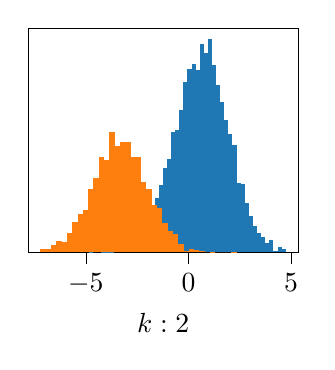
\begin{tikzpicture}

\definecolor{darkgray176}{RGB}{176,176,176}
\definecolor{darkorange25512714}{RGB}{255,127,14}
\definecolor{steelblue31119180}{RGB}{31,119,180}

\begin{axis}[
tick align=outside,
tick pos=left,
x grid style={darkgray176},
xlabel={$k:2$},
xmin=-7.80759693559219, xmax=5.34034850098321,
xtick style={color=black},
y grid style={darkgray176},
%ylabel={Frequency},
ymin=0, ymax=372.75,
%ytick style={color=black},
ytick=\empty,
scale=0.5
]
\draw[draw=none,fill=steelblue31119180] (axis cs:-4.84564394215464,0) rectangle (axis cs:-4.64588647216178,1);
\draw[draw=none,fill=steelblue31119180] (axis cs:-4.64588647216178,0) rectangle (axis cs:-4.44612900216892,0);
\draw[draw=none,fill=steelblue31119180] (axis cs:-4.44612900216892,0) rectangle (axis cs:-4.24637153217607,2);
\draw[draw=none,fill=steelblue31119180] (axis cs:-4.24637153217607,0) rectangle (axis cs:-4.04661406218321,1);
\draw[draw=none,fill=steelblue31119180] (axis cs:-4.04661406218321,0) rectangle (axis cs:-3.84685659219035,1);
\draw[draw=none,fill=steelblue31119180] (axis cs:-3.84685659219035,0) rectangle (axis cs:-3.64709912219749,1);
\draw[draw=none,fill=steelblue31119180] (axis cs:-3.64709912219749,0) rectangle (axis cs:-3.44734165220464,3);
\draw[draw=none,fill=steelblue31119180] (axis cs:-3.44734165220464,0) rectangle (axis cs:-3.24758418221178,4);
\draw[draw=none,fill=steelblue31119180] (axis cs:-3.24758418221178,0) rectangle (axis cs:-3.04782671221892,5);
\draw[draw=none,fill=steelblue31119180] (axis cs:-3.04782671221892,0) rectangle (axis cs:-2.84806924222607,9);
\draw[draw=none,fill=steelblue31119180] (axis cs:-2.84806924222606,0) rectangle (axis cs:-2.64831177223321,17);
\draw[draw=none,fill=steelblue31119180] (axis cs:-2.64831177223321,0) rectangle (axis cs:-2.44855430224035,25);
\draw[draw=none,fill=steelblue31119180] (axis cs:-2.44855430224035,0) rectangle (axis cs:-2.24879683224749,25);
\draw[draw=none,fill=steelblue31119180] (axis cs:-2.24879683224749,0) rectangle (axis cs:-2.04903936225464,41);
\draw[draw=none,fill=steelblue31119180] (axis cs:-2.04903936225464,0) rectangle (axis cs:-1.84928189226178,55);
\draw[draw=none,fill=steelblue31119180] (axis cs:-1.84928189226178,0) rectangle (axis cs:-1.64952442226892,70);
\draw[draw=none,fill=steelblue31119180] (axis cs:-1.64952442226892,0) rectangle (axis cs:-1.44976695227606,91);
\draw[draw=none,fill=steelblue31119180] (axis cs:-1.44976695227606,0) rectangle (axis cs:-1.25000948228321,112);
\draw[draw=none,fill=steelblue31119180] (axis cs:-1.25000948228321,0) rectangle (axis cs:-1.05025201229035,141);
\draw[draw=none,fill=steelblue31119180] (axis cs:-1.05025201229035,0) rectangle (axis cs:-0.850494542297493,156);
\draw[draw=none,fill=steelblue31119180] (axis cs:-0.850494542297493,0) rectangle (axis cs:-0.650737072304636,200);
\draw[draw=none,fill=steelblue31119180] (axis cs:-0.650737072304636,0) rectangle (axis cs:-0.450979602311778,203);
\draw[draw=none,fill=steelblue31119180] (axis cs:-0.450979602311778,0) rectangle (axis cs:-0.251222132318921,237);
\draw[draw=none,fill=steelblue31119180] (axis cs:-0.251222132318921,0) rectangle (axis cs:-0.0514646623260635,283);
\draw[draw=none,fill=steelblue31119180] (axis cs:-0.0514646623260635,0) rectangle (axis cs:0.148292807666794,305);
\draw[draw=none,fill=steelblue31119180] (axis cs:0.148292807666794,0) rectangle (axis cs:0.348050277659651,313);
\draw[draw=none,fill=steelblue31119180] (axis cs:0.348050277659651,0) rectangle (axis cs:0.547807747652509,303);
\draw[draw=none,fill=steelblue31119180] (axis cs:0.547807747652509,0) rectangle (axis cs:0.747565217645366,346);
\draw[draw=none,fill=steelblue31119180] (axis cs:0.747565217645366,0) rectangle (axis cs:0.947322687638223,332);
\draw[draw=none,fill=steelblue31119180] (axis cs:0.947322687638223,0) rectangle (axis cs:1.14708015763108,355);
\draw[draw=none,fill=steelblue31119180] (axis cs:1.14708015763108,0) rectangle (axis cs:1.34683762762394,312);
\draw[draw=none,fill=steelblue31119180] (axis cs:1.34683762762394,0) rectangle (axis cs:1.54659509761679,279);
\draw[draw=none,fill=steelblue31119180] (axis cs:1.54659509761679,0) rectangle (axis cs:1.74635256760965,250);
\draw[draw=none,fill=steelblue31119180] (axis cs:1.74635256760965,0) rectangle (axis cs:1.94611003760251,220);
\draw[draw=none,fill=steelblue31119180] (axis cs:1.94611003760251,0) rectangle (axis cs:2.14586750759537,197);
\draw[draw=none,fill=steelblue31119180] (axis cs:2.14586750759537,0) rectangle (axis cs:2.34562497758822,178);
\draw[draw=none,fill=steelblue31119180] (axis cs:2.34562497758822,0) rectangle (axis cs:2.54538244758108,115);
\draw[draw=none,fill=steelblue31119180] (axis cs:2.54538244758108,0) rectangle (axis cs:2.74513991757394,114);
\draw[draw=none,fill=steelblue31119180] (axis cs:2.74513991757394,0) rectangle (axis cs:2.9448973875668,82);
\draw[draw=none,fill=steelblue31119180] (axis cs:2.9448973875668,0) rectangle (axis cs:3.14465485755965,60);
\draw[draw=none,fill=steelblue31119180] (axis cs:3.14465485755965,0) rectangle (axis cs:3.34441232755251,44);
\draw[draw=none,fill=steelblue31119180] (axis cs:3.34441232755251,0) rectangle (axis cs:3.54416979754537,33);
\draw[draw=none,fill=steelblue31119180] (axis cs:3.54416979754537,0) rectangle (axis cs:3.74392726753822,26);
\draw[draw=none,fill=steelblue31119180] (axis cs:3.74392726753822,0) rectangle (axis cs:3.94368473753108,16);
\draw[draw=none,fill=steelblue31119180] (axis cs:3.94368473753108,0) rectangle (axis cs:4.14344220752394,21);
\draw[draw=none,fill=steelblue31119180] (axis cs:4.14344220752394,0) rectangle (axis cs:4.3431996775168,2);
\draw[draw=none,fill=steelblue31119180] (axis cs:4.3431996775168,0) rectangle (axis cs:4.54295714750965,9);
\draw[draw=none,fill=steelblue31119180] (axis cs:4.54295714750965,0) rectangle (axis cs:4.74271461750251,5);
\draw[draw=none,fill=darkorange25512714] (axis cs:-7.20996305211149,0) rectangle (axis cs:-6.95182942179264,6);
\draw[draw=none,fill=darkorange25512714] (axis cs:-6.95182942179264,0) rectangle (axis cs:-6.69369579147378,6);
\draw[draw=none,fill=darkorange25512714] (axis cs:-6.69369579147378,0) rectangle (axis cs:-6.43556216115493,12);
\draw[draw=none,fill=darkorange25512714] (axis cs:-6.43556216115493,0) rectangle (axis cs:-6.17742853083608,19);
\draw[draw=none,fill=darkorange25512714] (axis cs:-6.17742853083608,0) rectangle (axis cs:-5.91929490051723,18);
\draw[draw=none,fill=darkorange25512714] (axis cs:-5.91929490051722,0) rectangle (axis cs:-5.66116127019837,32);
\draw[draw=none,fill=darkorange25512714] (axis cs:-5.66116127019837,0) rectangle (axis cs:-5.40302763987952,50);
\draw[draw=none,fill=darkorange25512714] (axis cs:-5.40302763987952,0) rectangle (axis cs:-5.14489400956067,63);
\draw[draw=none,fill=darkorange25512714] (axis cs:-5.14489400956067,0) rectangle (axis cs:-4.88676037924181,71);
\draw[draw=none,fill=darkorange25512714] (axis cs:-4.88676037924181,0) rectangle (axis cs:-4.62862674892296,106);
\draw[draw=none,fill=darkorange25512714] (axis cs:-4.62862674892296,0) rectangle (axis cs:-4.37049311860411,123);
\draw[draw=none,fill=darkorange25512714] (axis cs:-4.37049311860411,0) rectangle (axis cs:-4.11235948828526,159);
\draw[draw=none,fill=darkorange25512714] (axis cs:-4.11235948828526,0) rectangle (axis cs:-3.8542258579664,153);
\draw[draw=none,fill=darkorange25512714] (axis cs:-3.8542258579664,0) rectangle (axis cs:-3.59609222764755,200);
\draw[draw=none,fill=darkorange25512714] (axis cs:-3.59609222764755,0) rectangle (axis cs:-3.3379585973287,177);
\draw[draw=none,fill=darkorange25512714] (axis cs:-3.3379585973287,0) rectangle (axis cs:-3.07982496700985,184);
\draw[draw=none,fill=darkorange25512714] (axis cs:-3.07982496700985,0) rectangle (axis cs:-2.82169133669099,184);
\draw[draw=none,fill=darkorange25512714] (axis cs:-2.82169133669099,0) rectangle (axis cs:-2.56355770637214,158);
\draw[draw=none,fill=darkorange25512714] (axis cs:-2.56355770637214,0) rectangle (axis cs:-2.30542407605329,159);
\draw[draw=none,fill=darkorange25512714] (axis cs:-2.30542407605329,0) rectangle (axis cs:-2.04729044573444,117);
\draw[draw=none,fill=darkorange25512714] (axis cs:-2.04729044573444,0) rectangle (axis cs:-1.78915681541558,105);
\draw[draw=none,fill=darkorange25512714] (axis cs:-1.78915681541558,0) rectangle (axis cs:-1.53102318509673,79);
\draw[draw=none,fill=darkorange25512714] (axis cs:-1.53102318509673,0) rectangle (axis cs:-1.27288955477788,73);
\draw[draw=none,fill=darkorange25512714] (axis cs:-1.27288955477788,0) rectangle (axis cs:-1.01475592445902,49);
\draw[draw=none,fill=darkorange25512714] (axis cs:-1.01475592445902,0) rectangle (axis cs:-0.756622294140172,36);
\draw[draw=none,fill=darkorange25512714] (axis cs:-0.756622294140172,0) rectangle (axis cs:-0.498488663821319,30);
\draw[draw=none,fill=darkorange25512714] (axis cs:-0.498488663821319,0) rectangle (axis cs:-0.240355033502467,14);
\draw[draw=none,fill=darkorange25512714] (axis cs:-0.240355033502467,0) rectangle (axis cs:0.0177785968163864,2);
\draw[draw=none,fill=darkorange25512714] (axis cs:0.0177785968163864,0) rectangle (axis cs:0.275912227135239,6);
\draw[draw=none,fill=darkorange25512714] (axis cs:0.275912227135239,0) rectangle (axis cs:0.534045857454092,4);
\draw[draw=none,fill=darkorange25512714] (axis cs:0.534045857454092,0) rectangle (axis cs:0.792179487772945,3);
\draw[draw=none,fill=darkorange25512714] (axis cs:0.792179487772945,0) rectangle (axis cs:1.0503131180918,0);
\draw[draw=none,fill=darkorange25512714] (axis cs:1.0503131180918,0) rectangle (axis cs:1.30844674841065,1);
\draw[draw=none,fill=darkorange25512714] (axis cs:1.30844674841065,0) rectangle (axis cs:1.5665803787295,0);
\draw[draw=none,fill=darkorange25512714] (axis cs:1.5665803787295,0) rectangle (axis cs:1.82471400904836,0);
\draw[draw=none,fill=darkorange25512714] (axis cs:1.82471400904836,0) rectangle (axis cs:2.08284763936721,0);
\draw[draw=none,fill=darkorange25512714] (axis cs:2.08284763936721,0) rectangle (axis cs:2.34098126968606,1);
\end{axis}

\end{tikzpicture}

			%\caption{Caption for second figure}
			\label{fig:2}
		\end{minipage}
		\hfill
		\begin{minipage}[htbp]{0.24\textwidth}
			\centering
			% This file was created with tikzplotlib v0.10.1.
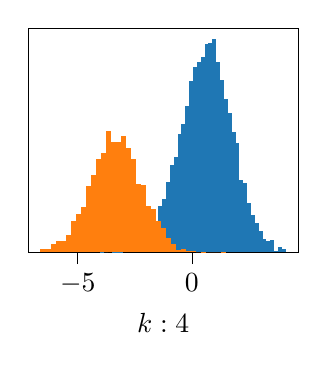
\begin{tikzpicture}

\definecolor{darkgray176}{RGB}{176,176,176}
\definecolor{darkorange25512714}{RGB}{255,127,14}
\definecolor{steelblue31119180}{RGB}{31,119,180}

\begin{axis}[
tick align=outside,
tick pos=left,
x grid style={darkgray176},
xlabel={$k:4$},
xmin=-7.16782843068525, xmax=4.65202446892355,
xtick style={color=black},
y grid style={darkgray176},
%ylabel={Frequency},
ymin=0, ymax=364.35,
%ytick style={color=black},
ytick=\empty,
scale=0.5
]
\draw[draw=none,fill=steelblue31119180] (axis cs:-4.01511339680388,0) rectangle (axis cs:-3.8457410671198,1);
\draw[draw=none,fill=steelblue31119180] (axis cs:-3.8457410671198,0) rectangle (axis cs:-3.67636873743571,0);
\draw[draw=none,fill=steelblue31119180] (axis cs:-3.67636873743571,0) rectangle (axis cs:-3.50699640775163,2);
\draw[draw=none,fill=steelblue31119180] (axis cs:-3.50699640775163,0) rectangle (axis cs:-3.33762407806754,1);
\draw[draw=none,fill=steelblue31119180] (axis cs:-3.33762407806754,0) rectangle (axis cs:-3.16825174838345,1);
\draw[draw=none,fill=steelblue31119180] (axis cs:-3.16825174838345,0) rectangle (axis cs:-2.99887941869937,1);
\draw[draw=none,fill=steelblue31119180] (axis cs:-2.99887941869937,0) rectangle (axis cs:-2.82950708901528,3);
\draw[draw=none,fill=steelblue31119180] (axis cs:-2.82950708901528,0) rectangle (axis cs:-2.6601347593312,4);
\draw[draw=none,fill=steelblue31119180] (axis cs:-2.6601347593312,0) rectangle (axis cs:-2.49076242964711,4);
\draw[draw=none,fill=steelblue31119180] (axis cs:-2.49076242964711,0) rectangle (axis cs:-2.32139009996302,8);
\draw[draw=none,fill=steelblue31119180] (axis cs:-2.32139009996302,0) rectangle (axis cs:-2.15201777027894,17);
\draw[draw=none,fill=steelblue31119180] (axis cs:-2.15201777027894,0) rectangle (axis cs:-1.98264544059485,27);
\draw[draw=none,fill=steelblue31119180] (axis cs:-1.98264544059485,0) rectangle (axis cs:-1.81327311091077,22);
\draw[draw=none,fill=steelblue31119180] (axis cs:-1.81327311091077,0) rectangle (axis cs:-1.64390078122668,43);
\draw[draw=none,fill=steelblue31119180] (axis cs:-1.64390078122668,0) rectangle (axis cs:-1.47452845154259,51);
\draw[draw=none,fill=steelblue31119180] (axis cs:-1.47452845154259,0) rectangle (axis cs:-1.30515612185851,76);
\draw[draw=none,fill=steelblue31119180] (axis cs:-1.30515612185851,0) rectangle (axis cs:-1.13578379217442,87);
\draw[draw=none,fill=steelblue31119180] (axis cs:-1.13578379217442,0) rectangle (axis cs:-0.966411462490336,114);
\draw[draw=none,fill=steelblue31119180] (axis cs:-0.966411462490336,0) rectangle (axis cs:-0.797039132806249,142);
\draw[draw=none,fill=steelblue31119180] (axis cs:-0.797039132806249,0) rectangle (axis cs:-0.627666803122163,155);
\draw[draw=none,fill=steelblue31119180] (axis cs:-0.627666803122163,0) rectangle (axis cs:-0.458294473438078,192);
\draw[draw=none,fill=steelblue31119180] (axis cs:-0.458294473438078,0) rectangle (axis cs:-0.288922143753991,208);
\draw[draw=none,fill=steelblue31119180] (axis cs:-0.288922143753991,0) rectangle (axis cs:-0.119549814069905,238);
\draw[draw=none,fill=steelblue31119180] (axis cs:-0.119549814069905,0) rectangle (axis cs:0.0498225156141805,278);
\draw[draw=none,fill=steelblue31119180] (axis cs:0.0498225156141805,0) rectangle (axis cs:0.219194845298267,302);
\draw[draw=none,fill=steelblue31119180] (axis cs:0.219194845298267,0) rectangle (axis cs:0.388567174982352,310);
\draw[draw=none,fill=steelblue31119180] (axis cs:0.388567174982352,0) rectangle (axis cs:0.557939504666439,317);
\draw[draw=none,fill=steelblue31119180] (axis cs:0.557939504666439,0) rectangle (axis cs:0.727311834350525,339);
\draw[draw=none,fill=steelblue31119180] (axis cs:0.727311834350525,0) rectangle (axis cs:0.89668416403461,341);
\draw[draw=none,fill=steelblue31119180] (axis cs:0.89668416403461,0) rectangle (axis cs:1.0660564937187,347);
\draw[draw=none,fill=steelblue31119180] (axis cs:1.0660564937187,0) rectangle (axis cs:1.23542882340278,310);
\draw[draw=none,fill=steelblue31119180] (axis cs:1.23542882340278,0) rectangle (axis cs:1.40480115308687,281);
\draw[draw=none,fill=steelblue31119180] (axis cs:1.40480115308687,0) rectangle (axis cs:1.57417348277095,249);
\draw[draw=none,fill=steelblue31119180] (axis cs:1.57417348277095,0) rectangle (axis cs:1.74354581245504,227);
\draw[draw=none,fill=steelblue31119180] (axis cs:1.74354581245504,0) rectangle (axis cs:1.91291814213913,195);
\draw[draw=none,fill=steelblue31119180] (axis cs:1.91291814213913,0) rectangle (axis cs:2.08229047182321,177);
\draw[draw=none,fill=steelblue31119180] (axis cs:2.08229047182321,0) rectangle (axis cs:2.2516628015073,117);
\draw[draw=none,fill=steelblue31119180] (axis cs:2.2516628015073,0) rectangle (axis cs:2.42103513119138,113);
\draw[draw=none,fill=steelblue31119180] (axis cs:2.42103513119138,0) rectangle (axis cs:2.59040746087547,81);
\draw[draw=none,fill=steelblue31119180] (axis cs:2.59040746087547,0) rectangle (axis cs:2.75977979055956,60);
\draw[draw=none,fill=steelblue31119180] (axis cs:2.75977979055956,0) rectangle (axis cs:2.92915212024364,47);
\draw[draw=none,fill=steelblue31119180] (axis cs:2.92915212024364,0) rectangle (axis cs:3.09852444992773,34);
\draw[draw=none,fill=steelblue31119180] (axis cs:3.09852444992773,0) rectangle (axis cs:3.26789677961181,22);
\draw[draw=none,fill=steelblue31119180] (axis cs:3.26789677961181,0) rectangle (axis cs:3.4372691092959,19);
\draw[draw=none,fill=steelblue31119180] (axis cs:3.4372691092959,0) rectangle (axis cs:3.60664143897999,20);
\draw[draw=none,fill=steelblue31119180] (axis cs:3.60664143897999,0) rectangle (axis cs:3.77601376866407,3);
\draw[draw=none,fill=steelblue31119180] (axis cs:3.77601376866407,0) rectangle (axis cs:3.94538609834816,8);
\draw[draw=none,fill=steelblue31119180] (axis cs:3.94538609834816,0) rectangle (axis cs:4.11475842803224,6);
\draw[draw=none,fill=darkorange25512714] (axis cs:-6.63056238979394,0) rectangle (axis cs:-6.41096241157501,6);
\draw[draw=none,fill=darkorange25512714] (axis cs:-6.41096241157501,0) rectangle (axis cs:-6.19136243335608,5);
\draw[draw=none,fill=darkorange25512714] (axis cs:-6.19136243335608,0) rectangle (axis cs:-5.97176245513715,14);
\draw[draw=none,fill=darkorange25512714] (axis cs:-5.97176245513715,0) rectangle (axis cs:-5.75216247691822,18);
\draw[draw=none,fill=darkorange25512714] (axis cs:-5.75216247691822,0) rectangle (axis cs:-5.53256249869928,18);
\draw[draw=none,fill=darkorange25512714] (axis cs:-5.53256249869928,0) rectangle (axis cs:-5.31296252048035,29);
\draw[draw=none,fill=darkorange25512714] (axis cs:-5.31296252048035,0) rectangle (axis cs:-5.09336254226142,51);
\draw[draw=none,fill=darkorange25512714] (axis cs:-5.09336254226142,0) rectangle (axis cs:-4.87376256404249,63);
\draw[draw=none,fill=darkorange25512714] (axis cs:-4.87376256404249,0) rectangle (axis cs:-4.65416258582356,73);
\draw[draw=none,fill=darkorange25512714] (axis cs:-4.65416258582356,0) rectangle (axis cs:-4.43456260760463,108);
\draw[draw=none,fill=darkorange25512714] (axis cs:-4.43456260760463,0) rectangle (axis cs:-4.2149626293857,125);
\draw[draw=none,fill=darkorange25512714] (axis cs:-4.2149626293857,0) rectangle (axis cs:-3.99536265116677,152);
\draw[draw=none,fill=darkorange25512714] (axis cs:-3.99536265116677,0) rectangle (axis cs:-3.77576267294784,161);
\draw[draw=none,fill=darkorange25512714] (axis cs:-3.77576267294784,0) rectangle (axis cs:-3.55616269472891,198);
\draw[draw=none,fill=darkorange25512714] (axis cs:-3.55616269472891,0) rectangle (axis cs:-3.33656271650998,179);
\draw[draw=none,fill=darkorange25512714] (axis cs:-3.33656271650998,0) rectangle (axis cs:-3.11696273829105,179);
\draw[draw=none,fill=darkorange25512714] (axis cs:-3.11696273829105,0) rectangle (axis cs:-2.89736276007212,189);
\draw[draw=none,fill=darkorange25512714] (axis cs:-2.89736276007212,0) rectangle (axis cs:-2.67776278185319,170);
\draw[draw=none,fill=darkorange25512714] (axis cs:-2.67776278185319,0) rectangle (axis cs:-2.45816280363426,151);
\draw[draw=none,fill=darkorange25512714] (axis cs:-2.45816280363426,0) rectangle (axis cs:-2.23856282541533,111);
\draw[draw=none,fill=darkorange25512714] (axis cs:-2.23856282541533,0) rectangle (axis cs:-2.01896284719639,109);
\draw[draw=none,fill=darkorange25512714] (axis cs:-2.01896284719639,0) rectangle (axis cs:-1.79936286897746,75);
\draw[draw=none,fill=darkorange25512714] (axis cs:-1.79936286897746,0) rectangle (axis cs:-1.57976289075853,71);
\draw[draw=none,fill=darkorange25512714] (axis cs:-1.57976289075853,0) rectangle (axis cs:-1.3601629125396,51);
\draw[draw=none,fill=darkorange25512714] (axis cs:-1.3601629125396,0) rectangle (axis cs:-1.14056293432067,40);
\draw[draw=none,fill=darkorange25512714] (axis cs:-1.14056293432067,0) rectangle (axis cs:-0.920962956101741,24);
\draw[draw=none,fill=darkorange25512714] (axis cs:-0.920962956101741,0) rectangle (axis cs:-0.701362977882811,13);
\draw[draw=none,fill=darkorange25512714] (axis cs:-0.701362977882811,0) rectangle (axis cs:-0.481762999663879,4);
\draw[draw=none,fill=darkorange25512714] (axis cs:-0.481762999663879,0) rectangle (axis cs:-0.262163021444949,5);
\draw[draw=none,fill=darkorange25512714] (axis cs:-0.262163021444949,0) rectangle (axis cs:-0.0425630432260187,3);
\draw[draw=none,fill=darkorange25512714] (axis cs:-0.0425630432260187,0) rectangle (axis cs:0.177036934992913,3);
\draw[draw=none,fill=darkorange25512714] (axis cs:0.177036934992913,0) rectangle (axis cs:0.396636913211843,0);
\draw[draw=none,fill=darkorange25512714] (axis cs:0.396636913211843,0) rectangle (axis cs:0.616236891430773,1);
\draw[draw=none,fill=darkorange25512714] (axis cs:0.616236891430773,0) rectangle (axis cs:0.835836869649705,0);
\draw[draw=none,fill=darkorange25512714] (axis cs:0.835836869649705,0) rectangle (axis cs:1.05543684786864,0);
\draw[draw=none,fill=darkorange25512714] (axis cs:1.05543684786864,0) rectangle (axis cs:1.27503682608757,0);
\draw[draw=none,fill=darkorange25512714] (axis cs:1.27503682608757,0) rectangle (axis cs:1.4946368043065,1);
\end{axis}

\end{tikzpicture}

			%\caption{Caption for third figure}
			\label{fig:3}
		\end{minipage}
		\hfill
		\begin{minipage}[htbp]{0.24\textwidth}
			\centering
			% This file was created with tikzplotlib v0.10.1.
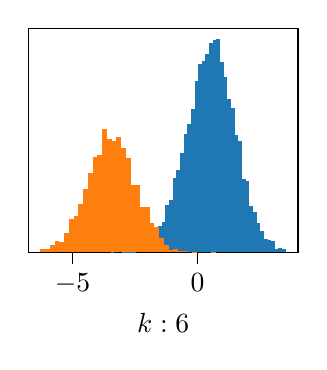
\begin{tikzpicture}

\definecolor{darkgray176}{RGB}{176,176,176}
\definecolor{darkorange25512714}{RGB}{255,127,14}
\definecolor{steelblue31119180}{RGB}{31,119,180}

\begin{axis}[
tick align=outside,
tick pos=left,
x grid style={darkgray176},
xlabel={$k:6$},
xmin=-6.77573066190925, xmax=4.02780843120382,
xtick style={color=black},
y grid style={darkgray176},
%ylabel={Frequency},
ymin=0, ymax=362.25,
ytick=\empty,
%ytick style={color=black},
scale=0.5
]
\draw[draw=none,fill=steelblue31119180] (axis cs:-3.4770362703687,0) rectangle (axis cs:-3.33091596322714,1);
\draw[draw=none,fill=steelblue31119180] (axis cs:-3.33091596322714,0) rectangle (axis cs:-3.18479565608559,0);
\draw[draw=none,fill=steelblue31119180] (axis cs:-3.18479565608559,0) rectangle (axis cs:-3.03867534894403,2);
\draw[draw=none,fill=steelblue31119180] (axis cs:-3.03867534894403,0) rectangle (axis cs:-2.89255504180248,1);
\draw[draw=none,fill=steelblue31119180] (axis cs:-2.89255504180248,0) rectangle (axis cs:-2.74643473466092,1);
\draw[draw=none,fill=steelblue31119180] (axis cs:-2.74643473466092,0) rectangle (axis cs:-2.60031442751937,1);
\draw[draw=none,fill=steelblue31119180] (axis cs:-2.60031442751937,0) rectangle (axis cs:-2.45419412037781,1);
\draw[draw=none,fill=steelblue31119180] (axis cs:-2.45419412037781,0) rectangle (axis cs:-2.30807381323626,5);
\draw[draw=none,fill=steelblue31119180] (axis cs:-2.30807381323626,0) rectangle (axis cs:-2.1619535060947,5);
\draw[draw=none,fill=steelblue31119180] (axis cs:-2.1619535060947,0) rectangle (axis cs:-2.01583319895314,7);
\draw[draw=none,fill=steelblue31119180] (axis cs:-2.01583319895315,0) rectangle (axis cs:-1.86971289181159,16);
\draw[draw=none,fill=steelblue31119180] (axis cs:-1.86971289181159,0) rectangle (axis cs:-1.72359258467004,27);
\draw[draw=none,fill=steelblue31119180] (axis cs:-1.72359258467004,0) rectangle (axis cs:-1.57747227752848,23);
\draw[draw=none,fill=steelblue31119180] (axis cs:-1.57747227752848,0) rectangle (axis cs:-1.43135197038692,43);
\draw[draw=none,fill=steelblue31119180] (axis cs:-1.43135197038692,0) rectangle (axis cs:-1.28523166324537,49);
\draw[draw=none,fill=steelblue31119180] (axis cs:-1.28523166324537,0) rectangle (axis cs:-1.13911135610381,77);
\draw[draw=none,fill=steelblue31119180] (axis cs:-1.13911135610381,0) rectangle (axis cs:-0.99299104896226,84);
\draw[draw=none,fill=steelblue31119180] (axis cs:-0.99299104896226,0) rectangle (axis cs:-0.846870741820704,120);
\draw[draw=none,fill=steelblue31119180] (axis cs:-0.846870741820704,0) rectangle (axis cs:-0.700750434679149,133);
\draw[draw=none,fill=steelblue31119180] (axis cs:-0.700750434679149,0) rectangle (axis cs:-0.554630127537594,160);
\draw[draw=none,fill=steelblue31119180] (axis cs:-0.554630127537594,0) rectangle (axis cs:-0.408509820396039,192);
\draw[draw=none,fill=steelblue31119180] (axis cs:-0.408509820396039,0) rectangle (axis cs:-0.262389513254484,207);
\draw[draw=none,fill=steelblue31119180] (axis cs:-0.262389513254484,0) rectangle (axis cs:-0.116269206112929,232);
\draw[draw=none,fill=steelblue31119180] (axis cs:-0.116269206112929,0) rectangle (axis cs:0.0298511010286262,277);
\draw[draw=none,fill=steelblue31119180] (axis cs:0.0298511010286262,0) rectangle (axis cs:0.175971408170181,304);
\draw[draw=none,fill=steelblue31119180] (axis cs:0.175971408170181,0) rectangle (axis cs:0.322091715311736,309);
\draw[draw=none,fill=steelblue31119180] (axis cs:0.322091715311736,0) rectangle (axis cs:0.468212022453292,321);
\draw[draw=none,fill=steelblue31119180] (axis cs:0.468212022453292,0) rectangle (axis cs:0.614332329594847,339);
\draw[draw=none,fill=steelblue31119180] (axis cs:0.614332329594847,0) rectangle (axis cs:0.760452636736401,344);
\draw[draw=none,fill=steelblue31119180] (axis cs:0.760452636736401,0) rectangle (axis cs:0.906572943877957,345);
\draw[draw=none,fill=steelblue31119180] (axis cs:0.906572943877957,0) rectangle (axis cs:1.05269325101951,307);
\draw[draw=none,fill=steelblue31119180] (axis cs:1.05269325101951,0) rectangle (axis cs:1.19881355816107,283);
\draw[draw=none,fill=steelblue31119180] (axis cs:1.19881355816107,0) rectangle (axis cs:1.34493386530262,248);
\draw[draw=none,fill=steelblue31119180] (axis cs:1.34493386530262,0) rectangle (axis cs:1.49105417244418,233);
\draw[draw=none,fill=steelblue31119180] (axis cs:1.49105417244418,0) rectangle (axis cs:1.63717447958573,189);
\draw[draw=none,fill=steelblue31119180] (axis cs:1.63717447958573,0) rectangle (axis cs:1.78329478672729,180);
\draw[draw=none,fill=steelblue31119180] (axis cs:1.78329478672729,0) rectangle (axis cs:1.92941509386884,118);
\draw[draw=none,fill=steelblue31119180] (axis cs:1.92941509386884,0) rectangle (axis cs:2.0755354010104,115);
\draw[draw=none,fill=steelblue31119180] (axis cs:2.0755354010104,0) rectangle (axis cs:2.22165570815195,75);
\draw[draw=none,fill=steelblue31119180] (axis cs:2.22165570815195,0) rectangle (axis cs:2.36777601529351,65);
\draw[draw=none,fill=steelblue31119180] (axis cs:2.36777601529351,0) rectangle (axis cs:2.51389632243506,48);
\draw[draw=none,fill=steelblue31119180] (axis cs:2.51389632243506,0) rectangle (axis cs:2.66001662957662,35);
\draw[draw=none,fill=steelblue31119180] (axis cs:2.66001662957662,0) rectangle (axis cs:2.80613693671817,22);
\draw[draw=none,fill=steelblue31119180] (axis cs:2.80613693671817,0) rectangle (axis cs:2.95225724385973,20);
\draw[draw=none,fill=steelblue31119180] (axis cs:2.95225724385973,0) rectangle (axis cs:3.09837755100128,18);
\draw[draw=none,fill=steelblue31119180] (axis cs:3.09837755100128,0) rectangle (axis cs:3.24449785814284,5);
\draw[draw=none,fill=steelblue31119180] (axis cs:3.24449785814284,0) rectangle (axis cs:3.39061816528439,7);
\draw[draw=none,fill=steelblue31119180] (axis cs:3.39061816528439,0) rectangle (axis cs:3.53673847242595,6);
\draw[draw=none,fill=darkorange25512714] (axis cs:-6.28466070313138,0) rectangle (axis cs:-6.09454834083815,6);
\draw[draw=none,fill=darkorange25512714] (axis cs:-6.09454834083815,0) rectangle (axis cs:-5.90443597854491,5);
\draw[draw=none,fill=darkorange25512714] (axis cs:-5.90443597854491,0) rectangle (axis cs:-5.71432361625168,12);
\draw[draw=none,fill=darkorange25512714] (axis cs:-5.71432361625168,0) rectangle (axis cs:-5.52421125395844,19);
\draw[draw=none,fill=darkorange25512714] (axis cs:-5.52421125395844,0) rectangle (axis cs:-5.33409889166521,17);
\draw[draw=none,fill=darkorange25512714] (axis cs:-5.33409889166521,0) rectangle (axis cs:-5.14398652937197,31);
\draw[draw=none,fill=darkorange25512714] (axis cs:-5.14398652937197,0) rectangle (axis cs:-4.95387416707874,54);
\draw[draw=none,fill=darkorange25512714] (axis cs:-4.95387416707874,0) rectangle (axis cs:-4.7637618047855,59);
\draw[draw=none,fill=darkorange25512714] (axis cs:-4.7637618047855,0) rectangle (axis cs:-4.57364944249227,78);
\draw[draw=none,fill=darkorange25512714] (axis cs:-4.57364944249227,0) rectangle (axis cs:-4.38353708019903,102);
\draw[draw=none,fill=darkorange25512714] (axis cs:-4.38353708019903,0) rectangle (axis cs:-4.1934247179058,128);
\draw[draw=none,fill=darkorange25512714] (axis cs:-4.1934247179058,0) rectangle (axis cs:-4.00331235561256,154);
\draw[draw=none,fill=darkorange25512714] (axis cs:-4.00331235561256,0) rectangle (axis cs:-3.81319999331933,158);
\draw[draw=none,fill=darkorange25512714] (axis cs:-3.81319999331933,0) rectangle (axis cs:-3.62308763102609,200);
\draw[draw=none,fill=darkorange25512714] (axis cs:-3.62308763102609,0) rectangle (axis cs:-3.43297526873286,183);
\draw[draw=none,fill=darkorange25512714] (axis cs:-3.43297526873286,0) rectangle (axis cs:-3.24286290643962,180);
\draw[draw=none,fill=darkorange25512714] (axis cs:-3.24286290643962,0) rectangle (axis cs:-3.05275054414639,186);
\draw[draw=none,fill=darkorange25512714] (axis cs:-3.05275054414639,0) rectangle (axis cs:-2.86263818185316,168);
\draw[draw=none,fill=darkorange25512714] (axis cs:-2.86263818185316,0) rectangle (axis cs:-2.67252581955992,153);
\draw[draw=none,fill=darkorange25512714] (axis cs:-2.67252581955992,0) rectangle (axis cs:-2.48241345726669,109);
\draw[draw=none,fill=darkorange25512714] (axis cs:-2.48241345726669,0) rectangle (axis cs:-2.29230109497345,109);
\draw[draw=none,fill=darkorange25512714] (axis cs:-2.29230109497345,0) rectangle (axis cs:-2.10218873268022,74);
\draw[draw=none,fill=darkorange25512714] (axis cs:-2.10218873268022,0) rectangle (axis cs:-1.91207637038698,74);
\draw[draw=none,fill=darkorange25512714] (axis cs:-1.91207637038698,0) rectangle (axis cs:-1.72196400809375,48);
\draw[draw=none,fill=darkorange25512714] (axis cs:-1.72196400809375,0) rectangle (axis cs:-1.53185164580051,41);
\draw[draw=none,fill=darkorange25512714] (axis cs:-1.53185164580051,0) rectangle (axis cs:-1.34173928350728,23);
\draw[draw=none,fill=darkorange25512714] (axis cs:-1.34173928350728,0) rectangle (axis cs:-1.15162692121404,12);
\draw[draw=none,fill=darkorange25512714] (axis cs:-1.15162692121404,0) rectangle (axis cs:-0.961514558920808,4);
\draw[draw=none,fill=darkorange25512714] (axis cs:-0.961514558920808,0) rectangle (axis cs:-0.771402196627573,6);
\draw[draw=none,fill=darkorange25512714] (axis cs:-0.771402196627573,0) rectangle (axis cs:-0.581289834334338,2);
\draw[draw=none,fill=darkorange25512714] (axis cs:-0.581289834334338,0) rectangle (axis cs:-0.391177472041103,3);
\draw[draw=none,fill=darkorange25512714] (axis cs:-0.391177472041103,0) rectangle (axis cs:-0.201065109747868,0);
\draw[draw=none,fill=darkorange25512714] (axis cs:-0.201065109747868,0) rectangle (axis cs:-0.0109527474546338,1);
\draw[draw=none,fill=darkorange25512714] (axis cs:-0.0109527474546338,0) rectangle (axis cs:0.179159614838601,0);
\draw[draw=none,fill=darkorange25512714] (axis cs:0.179159614838601,0) rectangle (axis cs:0.369271977131836,0);
\draw[draw=none,fill=darkorange25512714] (axis cs:0.369271977131836,0) rectangle (axis cs:0.559384339425071,0);
\draw[draw=none,fill=darkorange25512714] (axis cs:0.559384339425071,0) rectangle (axis cs:0.749496701718305,1);
\end{axis}

\end{tikzpicture}

			%\caption{Caption for fourth figure}
			\label{fig:4}
		\end{minipage}
		\caption{Residuals with respect to $\mathbb{P}$ and $\mathbb{Q}$, $k$ represents optimization step.}
		\label{fig:normal-residual}
	\end{figure}

	\subsection{Proof of Theorem~\ref{thm:improvement-of-theta}}
	\label{app:improvement-of-theta}
	\begin{proof}
		To show the change in $\varepsilon$ we will first calculate the expected change in $\vtheta$ by the $\vtheta$-update described in Equation \ref{eqn:theta-update}. We will also introduce some notation, $\mathcal{S}$ represents all $\vx \in X$ that are within the lowest $np$ losses, i.e. within the subquantile, $\vp \in \mathcal{S}$ represent all data vectors from $\mathbb{P}$ that are within the SubQuantile, similarly $\vq \in \mathbb{Q}$ represent all data vectors from $\mathbb{Q}$ that are within the SubQuantile. Furthermore, $|\mathcal{S}| = np$, there are $\varepsilon n$ points from $\mathbb{Q}$ in $\mathcal{S}$ and $(1-\varepsilon)n$ points from $\mathbb{P}$ within $\mathcal{S}$. 
		\begingroup
		%\addtolength{\jot}{0.5em}
		\begin{align*}
			\mathbb{E}\left[\vtheta_{k+1}\right] &= \vtheta_k - \mathbb{E}\left[\alpha \nabla g(\vtheta_k,t_{k+1})\right] &&\\
			&= \vtheta_k - \alpha \mathbb{E}\left[\sum_{\vx \in \mathcal{S}}\vx(\vtheta^T\vx - y) \right] &&\\
			&= \vtheta_k - \alpha \mathbb{E}\left[\sum_{\vx \in \mathcal{S}}\vx\vx^T\vtheta_k - \vx y \right] &&\\
			&= \vtheta_k - \alpha \mathbb{E}\left[\sum_{\vp \in \mathcal{S}}\vp\vp^T\vtheta_k - \vp y_p + \sum_{\vq \in \mathcal{S}} \vq\vq^T\vtheta_k - \vq y_q \right] &&
			\intertext{We will use Assumption \ref{asm:normal-corruption} to rewrite $y_p$ and $y_q$}
			&= \vtheta_k - \alpha \mathbb{E}\left[\sum_{\vp \in \mathcal{S}}\vp\vp^T\vtheta_k - \vp (\vbeta_P \vp + \eps_P) + \sum_{\vq \in \mathcal{S}} \vq\vq^T\vtheta_k - \vq (\vbeta_Q \vp + \eps_Q) \right] &&\\
			&= \vtheta_k - \alpha\left(\sum_{\vp \in \mathcal{S}} \left(\vmu \vmu^T + \Sigma\right)\vtheta_k - \left(\vmu \vmu^T + \Sigma\right)\vbeta_P - \sum_{\vq \in \mathcal{S}} \left(\vmu \vmu^T + \Sigma\right)\vtheta_k + \left(\vmu \vmu^T + \Sigma\right)\vbeta_Q\right) &&
		\end{align*}
		 \vspace{1em}
		\begin{equation}\vspace{1em}
			\mathbb{E}\left[\vtheta_{(t+1)}\right]= \vtheta_{(t)} - \alpha np \mC\left(\vtheta_{(t)} - (1-\varepsilon)\vbeta_P - \varepsilon\vbeta_Q\right) 
		\end{equation}
		
		\endgroup
		Now that we have the expected update for $\vtheta$ in terms of the linear regression coefficients, we now want to utilize Lemma \ref{lem:effect-of-projection}.\\
		Let $\displaystyle \vtheta_k = \alpha_1\vbeta_P + \alpha_2\vbeta_Q + \sum_{i=3}^{d}\alpha_i \vr_i$ in the same basis $\mB$ defined in Lemma \ref{lem:effect-of-projection}. Note in the case of data that is normally distributed about $0$ with no covariance amongst the predictor variables, then $\mC$ is a multiple of the identity. If we proprocess the data using a standard normal scalar such that all features follow a $\mathcal{N}(0,1)$ distribution, then we can assume it follows $\displaystyle \mC = (\vzero\vzero^T + I) = I$. Let $\gamma \coloneqq \alpha np$. Then the following manipulations hold:
		\begin{align*}
			\mathbb{E}\left[\vtheta_{(t+1)}\right] &= \vtheta_{(t)} - \gamma\left(\vtheta_{(t)} - (1-\varepsilon^{(t)})\vbeta_P - \varepsilon^{(t)} \vbeta_Q\right) &&\\
			&= \vtheta_{(t)}(1-\gamma) + \gamma (1-\varepsilon^{(t)})\vbeta_P + (1-\gamma)\varepsilon^{(t)}\vbeta_Q &&\\
			&= (1-\gamma)\left(\alpha_1 \vbeta_P + \alpha_2^{(t)} \vbeta_Q + \sum_{i=3}^d\alpha_i^{(t)}\vr_i\right) + \gamma(1-\varepsilon^{(t)})\vbeta_P + \gamma\varepsilon^{(t)}\vbeta_Q &&\\
			&= \left(\alpha_1^{(t)}(1-\gamma) + \gamma(1-\varepsilon^{(t)})\right)\vbeta_P + \left(\alpha_2^{(t)}(1-\gamma) + \gamma \varepsilon^{(t)}\right)\vbeta_Q + (1-\gamma)\sum_{i=3}^d\alpha_i^{(t)}\vr_i &&
		\end{align*}
		We will now calculate the difference. 
		\begin{align*}
			\mathbb{E}\left[\vtheta_{(t+1)} - \vtheta_{(t)}\right] &= \left(-\gamma\alpha_1^{(t)} + \gamma(1-\varepsilon^{(t)})\right)\vbeta_P + \left(-\gamma \alpha_2^{(t)} + \gamma \varepsilon^{(t)}\right)\vbeta_Q + (1-\gamma)\sum_{i=3}^d\alpha_i^{(t)}\vr_i &&\\
			&= \gamma\left((1-\varepsilon^{(t)}) - \alpha_1^{(t)}\right)\vbeta_P + \gamma\left(\varepsilon^{(t)} - \alpha_2^{(t)}\right)\vbeta_Q + (1-\gamma)\sum_{i=3}^d\alpha_i^{(t)}\vr_i &&
		\end{align*}
		Thus the conditions for $\varepsilon$ to decrease by expectation are:
		\begin{equation}
			\norm{\left((1-\varepsilon^{(t)}) - \alpha_1^{(t)}\right)\vbeta_P} > \norm{\left(\varepsilon^{(t)} - \alpha_2^{(t)}\right)\vbeta_Q}
		\end{equation}  
		This concludes the proof. 
	\end{proof}

	\subsection{Proof of Theorem ~\ref{thm:probability-epsilon-decreasing}}
	\label{app:decrease-of-epsilon}
	\begin{proof}
		To calculate the probability $\varepsilon^{(t+1)} < \varepsilon^{(t)}$, we will first calculate $\mathbb{E}\left[\varepsilon^{(t+1)}\right]$. We will start by calculating the expectation of the loss. 
		\begin{align*}
			\mathbb{E}\left[\left(\vtheta_{(t+1)}^T\vp_i - y_i\right)^2\right] &= \mathbb{E}\left[\vtheta_{(t+1)}^T\vp_i - y_i\right]^2 + \Var\left(\vtheta_{(t+1)}^T\vp_i - y_i\right) &&\\
			&= \mathbb{E}\left[\vtheta_{(t+1)}^T\vp_i - \vbeta_P^T\vp_i - \eps_P\right]^2 + \Var\left(\vtheta_{(t+1)}^T\vp_i - \vbeta_P^T\vp_i - \eps_P\right) &&\\
			&= \left(\left(\vtheta^T_{(t+1)} - \vbeta_P^T\right)\mathbb{E}\left[\vp_i\right]\right)^2 + \Var\left(\left(\vtheta^T_{(t+1)}-\vbeta_P^T\right)\vp_i\right) + \Var\left(\eps_P\right)	&&\\	
			&= \left(\left(\vtheta^T_{(t+1)}-\vbeta_P^T\right)\vmu\right)^2 + \left(\vtheta^T_{(t+1)} - \vbeta_P^T\right)\Sigma\left(\vtheta_{(t+1)} - \vbeta_P\right) + \Var\left(\eps_P\right)
		\end{align*}
		It thus follows similarly:
		\begin{equation*}
			\mathbb{E}\left[\left(\vtheta_{(t+1)}^T\vq_i - y_i\right)^2\right] =  \left(\left(\vtheta^T_{(t+1)}-\vbeta_Q^T\right)\vmu\right)^2 + \left(\vtheta^T_{(t+1)} - \vbeta_Q^T\right)\Sigma\left(\vtheta_{(t+1)} - \vbeta_Q\right) + \Var\left(\eps_Q\right)
		\end{equation*}
		To simplify our notation, let $\zeta_P \coloneqq \mathbb{E}\left[\left(\vtheta_{(t+1)}^T\vp_i - y_i\right)^2\right]$ and $\zeta_Q \coloneqq \mathbb{E}\left[\left(\vtheta_{(t+1)}^T\vq_i - y_i\right)^2\right]$ and let $\eta_P \coloneqq \mathbb{E}\left[\vtheta_{(t+1)}^T\vp_i - y_i\right]$ and $\eta_Q \coloneqq \mathbb{E}\left[\vtheta_{(t+1)}^T\vq_i - y_i\right]$
		We are now interested in calculating the variance of the loss. \\
		Let $\sigma^2_P \coloneqq \Var\left(\vtheta^T_{(t+1)}\vp_i - y_i\right) = \left(\vtheta^T_{(t+1)} - \vbeta_P^T\right)\Sigma\left(\vtheta_{(t+1)} - \vbeta_P\right) + \Var\left(\eps_P\right)$. 
		\begin{align*}
			\Var\left(\left(\vtheta_{(t+1)}^T\vp_i - y_i\right)^2\right)&= \mathbb{E}\left[\left(\vtheta_{(t+1)}^T\vp_i - y_i\right)^4\right] - \mathbb{E}\left[\left(\vtheta_{(t+1)}^T\vp_i - y_i\right)^2\right]^2 &&\\
			&= \mathbb{E}\left[\vtheta_{(t+1)}^T\vp_i - y_i\right]^4 + 6 \mathbb{E}\left[\vtheta_{(t+1)}^T\vp_i - y_i\right]^2\sigma_P^2 + 3\sigma_P^4 - \zeta_P^2&&\\
			&= \eta_P^4 + 6 \eta_P^2 \sigma_P^2 + 3\sigma_P^4 - \zeta_P^2 &&
		\end{align*}
		It similarly follows:
		\begin{align*}
			\Var\left(\left(\vtheta_{(t+1)}^T\vq_i - y_i\right)^2\right)&=\eta_Q^4 + 6 \eta_Q^2 \sigma_Q^2 + 3\sigma_Q^4 - \zeta_Q^2 &&
		\end{align*}
		Recall that the expected value of $\varepsilon^{(t+1)}$ is equal to the expected number of elements from $Q$ within the $p$-Quantile, $\mathcal{Q}_p$. So we will now calculate $\mathcal{Q}_p$. To this we will utilize the  loss of the distribution. 
		\begin{align*}
			\mathbb{E}\left[\left(\vtheta_{(t+1)}^T \vx_i - y_i\right)^2\right] &= (1-\varepsilon^{(t)})\mathbb{E}\left[\left(\vtheta_{(t+1)}^T \vp_i - y_i\right)^2\right] + \varepsilon^{(t)}\mathbb{E}\left[\left(\vtheta_{(t+1)}^T \vq_i - y_i\right)^2\right] &&\\
			&= (1-\varepsilon^{(t)})\zeta_P + \varepsilon^{(t)}\zeta_Q &&
		\end{align*}
		\begin{align*}
			\Var\left(\left(\vtheta_{(t+1)}^T\vx_i - y_i\right)^2\right) &= (1-\varepsilon^{(t)})^2\Var\left(\left(\vtheta_{(t+1)}^T\vp_i - y_i\right)^2\right) + \varepsilon^{(t)2}\Var\left(\left(\vtheta_{(t+1)}^T\vq_i - y_i\right)^2\right) &&\\
			&= (1-\varepsilon^{(t)})^2\left(\eta_P^4 + 6 \eta_P^2 \sigma_P^2 + 3\sigma_P^4 - \zeta_P^2\right) + (\varepsilon^{(t)})^2\left(\eta_Q^4 + 6 \eta_Q^2 \sigma_Q^2 + 3\sigma_Q^4 - \zeta_Q^2\right) &&
		\end{align*}
		It thus follows $\displaystyle \left(\vtheta_{(t+1)}^T\vq_i - y_i\right)$ follows a $\chi^2$ distribution with $1$ degree of freedom and \begin{equation*} \lambda = \frac{\zeta_Q}{\eta_Q^4 + 6 \eta_Q^2 \sigma_Q^2 + 3\sigma_Q^4 - \zeta_Q^2}\end{equation*}
		Let $\mathcal{Q}_p^{(t+1)}$ be given as the $np$ greatest loss of the data, i.e. $\mathcal{Q}_p^{(t+1)} = \vnu_{np}^{(t+1)}$. It then follows:
		\begin{equation*}
			\mathbb{P}\left[\left(\vtheta^T_{(t+1)}\vq_i -y_i\right)^2 \leq \mathcal{Q}_p\right] = 1 - Q_{1}\left(\sqrt{\lambda},\sqrt{\mathcal{Q}_p}\right)
		\end{equation*}
		It thus follows:
		\begin{equation*}
			\mathbb{E}\left[\varepsilon^{(t+1)}\right] = 1 - Q_{1}\left(\sqrt{\lambda},\sqrt{\mathcal{Q}_p}\right)
		\end{equation*}
		Now we can calculate the probability of improvement per iteration by invoking Markov's Inequality:
		\begin{align*}
			\mathbb{P}\left[\varepsilon^{(t+1)} \geq \varepsilon^{(t)}\right] &\leq \frac{\mathbb{E}\left[\varepsilon^{(t+1)}\right]}{\varepsilon^{(t)}} &&\\
			&= \frac{1 - Q_{1}\left(\sqrt{\lambda},\sqrt{\mathcal{Q}_p}\right)}{\varepsilon^{(t)}}
		\end{align*}
		It thus follows:
		\begin{align*}
			\mathbb{P}\left[\varepsilon^{(t+1)} \leq \varepsilon^{(t)}\right] &\geq 1 - \frac{1 - Q_{1}\left(\sqrt{\lambda},\sqrt{\mathcal{Q}_p}\right)}{\varepsilon^{(t)}}
		\end{align*} 
	\end{proof}
	This concludes the proof.
	\newpage
	
	\section{Proofs for Convergence}
	\label{app:convergence-proofs}
	\subsection{Proof of Theorem ~\ref{thm:convergence-guarantee}}
	\begin{proof}
	We will first start by introducing new notation. Let $S$ represent a matrix with $np$ data points from $X$, in other words it is a possible SubQuantile Matrix. Let $\displaystyle\vPi$ represent the set of all such possible matrices $S$ of $X$. Note $\displaystyle \left|\vPi\right| = \binom{n}{np}$. We can now redefine the min-max optimization problem of $g$ to a min-min optimization problem. Let us define the function $f(\vtheta, S) = \norm{\vtheta^T S - y_S}_2^2$
	\begin{equation}
		\vtheta^*, S^* = \argmin_{\vtheta \in \mathbb{R}^d} \argmin_{S \in \vPi} \norm{\vtheta^T S - y_S}_2^2
	\end{equation}
	Note we have a $\mathcal{O}(n)$ oracle for the $\displaystyle \argmin_{S\in \vPi}f(\vtheta_T,S_T)$. 
	\begin{restatable}{lemma}{unique-S-minimizer}
		\label{lem:unique-S-minimizer}
		The resultant $\displaystyle \widetilde{S} = \argmin_{S \in \vPi} f(\vtheta,S)$ is a unique minimizer iff all points in $X$ are different. 
	\end{restatable}
	We will now show $f$ is a monotonically decreasing function.\\
	First let us define $\phi(\cdot) = \min_{S \in \vPi}\left(\cdot,S\right)$. 
	Let us also note $f$ is $\ell$ smooth with respect to $\vtheta$. This is following notation from \cite{Jin_2019}.It thus follows:
	\begin{align*}
		f(\vtheta_{k+1}, S_k) &\leq f(\vtheta_k, S_k) + \langle\nabla_\vtheta f(\vtheta_k,S_k), \vtheta_{k+1}-\vtheta_k \rangle + \frac{\ell}{2}\norm{\vtheta_{k+1}-\vtheta_k}_2^2 &&\\
		&= \phi(\vtheta_k) + \langle\nabla_\vtheta f(\vtheta_k,S_k), -\frac{1}{\ell}\nabla_\vtheta f(\vtheta_k,S_k)\rangle + \frac{\ell}{2}\norm{\frac{1}{\ell}\nabla_\vtheta f(\vtheta_k,S_k)}_2^2 &&\\
		&= \phi(\vtheta_k) - \frac{1}{\ell}\left(\nabla_\vtheta f(\vtheta_k,S_k)\right)^2 + \frac{1}{2\ell}\left(\nabla_\vtheta f(\vtheta_k,S_k)\right)^2 &&\\
		&= \phi(\vtheta_k) - \frac{1}{2\ell}\left(\nabla_\vtheta f(\vtheta_k,S_k)\right)^2 &&\\
	\end{align*} 
	Thus we have proved the inner optimization problem is monotonically decreasing. Since the outer minimization is strictly less than or equal to the result from the inner optimization, it follows after each two step optimization: 
	\begin{align*}
		\phi(\vtheta_{k+1}) \leq \phi(\vtheta_k)
	\end{align*}
	
	Since $f$ is lower bounded by $0$. We can invoke Montonicity Convergence Theorem, since $f$ is a monotically decreasing function and is lower bounded, it therefore converges to either a local or global minimum. 
	\end{proof}
	
	\subsection{Expectation of Improvement}
	We are also interested in expected improvement after the Subquantile matrix update. 
	\begin{align*}
		\mathbb{E}&\left[f\left(\vtheta_{(k)}, S^{(k+1)}\right) - f\left(\vtheta_{(k)}, S^{(k)}\right)\right] = \mathbb{E}\left[\varepsilon^{(t)} - \varepsilon^{(t-1)}\right]\mathbb{E}\left[\sum_{i=1}^{n(\varepsilon^{(t)}-\varepsilon^{(t-1)})}\norm{\vtheta_{(k)}^T\vp_i -y_i}_2^2 - \norm{\vtheta_{(k)}^T\vq_i - y_i}_2^2\right] &&\\
		&= \mathbb{E}\left[\varepsilon^{(t)} - \varepsilon^{(t-1)}\right]\mathbb{E}\left[\sum_{i=1}^{n(\varepsilon^{(t)}-\varepsilon^{(t-1)})}\norm{\vtheta_{(k)}^T\vp_i -y_i}_2^2 - \norm{\vtheta_{(k)}^T\vq_i - y_i}_2^2\right] &&
	\end{align*}
	We can now use reverse triangle inequality.
	\begin{align*}
		&\leq \mathbb{E}\left[\varepsilon^{(t)} - \varepsilon^{(t-1)}\right] \mathbb{E}\left[\sum_{i=1}^{n\left(\varepsilon^{(t)}-\varepsilon^{(t-1)}\right)}\norm{\vtheta_{(k)}^T\vp_i - \vbeta_P\vp_i - \eps_P - \vtheta^T_{(k)}\vq_i + \vbeta_Q\vq_i + \eps_Q}_2^2 \right] &&\\
		&= \mathbb{E}\left[\varepsilon^{(t)} - \varepsilon^{(t-1)}\right] \mathbb{E}\left[\sum_{i=1}^{n\left(\varepsilon^{(t)}-\varepsilon^{(t-1)}\right)}\norm{\left(\vtheta^T_{(k)} - \vbeta_P\right)\vp_i + \left(\vbeta_Q - \vtheta^T_{(k)}\right)\vq_i - \eps_P+ \eps_Q}_2^2 \right] &&
	\end{align*}
	Now we can use theorem \ref{thm:expected-value-corrupted}. To simplify notation, let $\Xi \triangleq \mathbb{E}\left[\varepsilon^{(t)} - \varepsilon^{(t-1)}\right]$
	\begin{align*}
		&= \Xi \mathbb{E}\left[\sum_{i=1}^{n\Xi}\norm{\left((1-\varepsilon^{(t)})\vbeta_P + \varepsilon^{(t)}\vbeta_Q - \vbeta_P\right)\vp_i + \left(\vbeta_Q - (1 - \varepsilon^{(t)})\vbeta_P - \varepsilon^{(t)}\vbeta_Q \right)q_i - \eps_P+ \eps_Q}_2^2 \right] &&\\
		&= \Xi \mathbb{E}\left[\sum_{i=1}^{n\Xi}\norm{\left(-\varepsilon^{(t)}\vbeta_P + \varepsilon^{(t)}\vbeta_Q\right)\vp_i + \left((1 - \varepsilon^{(t)})\vbeta_Q - (1 - \varepsilon^{(t)})\vbeta_P\right)\vq_i - \eps_P+ \eps_Q}_2^2 \right] &&\\
		&= \Xi \mathbb{E}\left[\sum_{i=1}^{n\Xi}\norm{\varepsilon^{(t)}\left(\vbeta_Q - \vbeta_P\right)\vp_i + (1 - \varepsilon^{(t)})\left(\vbeta_Q - \vbeta_P\right)\vq_i - \eps_P+ \eps_Q}_2^2 \right] &&
	\end{align*}
	Here we can use the fact that $\mathbb{E}\left[X^2\right] = \mathbb{E}\left[X\right]^2 + \Var(X)$ for a random variable $X$

	\bigskip
	Let us define the function $h(\vtheta_k) = f(\vtheta_k,S_{k-1}) - f(\vtheta_k,S_k)$, a strictly non-negative function. From our results above it follows:
	\begin{align*}
		\phi(\vtheta_{k+1}) &\leq \phi(\vtheta_k) - \frac{1}{2\ell}\left(\nabla_\vtheta f(\vtheta_k,S_k)\right)^2 &&\\
		&= f(\vtheta_k, S_{k-1}) - h(\vtheta_k) +  - \frac{\ell}{2}\norm{\vtheta_{k+1} - \vtheta_k}^2_2 \\
		&= f(\vtheta_k, S_{k-1}) - h(\vtheta_k) - \frac{\ell}{2}\norm{\vtheta_{k+1} - \frac{1}{\ell} \nabla_\vtheta f(\vtheta_k,S_k) - \vtheta_k}_2^2 &&\\
		&= f(\vtheta_k, S_{k-1}) - h(\vtheta_k) - \frac{\ell}{2}\left(\norm{\vtheta_{k+1}-\vtheta_k}_2^2 + \frac{2}{\ell}\norm{\vtheta_{k+1}-\vtheta_k}\nabla_\vtheta f(\vtheta_k,S_k) + \frac{1}{\ell^2}\nabla_\vtheta f(\vtheta_k,S_k)\right)
	\end{align*}
	\newpage
	
	\section{Stochastic Sub-Quantile Optimization}
	In the age of big data, stochastic methods are necessary for fast training of models to handle large amounts of data. In this section we provide an algorithm for Stochastic Sub-Quantile Optimization.
	\begin{algorithm}[H]
		\DontPrintSemicolon
		
		\KwInput{Training iterations $T$, Quantile $p$, Corruption Percentage $\eps$, Input Parameters $d$, Batch Size $m$}
		\KwOutput{Trained Parameters, $\displaystyle \vtheta$}
		$\vtheta_1 \gets \mathcal{N}(0,\sigma)^d$\\
		\For{$k \in 1,2,\ldots,T$}
		{
			$I \subseteq \left[n\right]$ of size $m$\\
			$\displaystyle \vnu = \left(X_I\vtheta_k - y_I\right)^2$\\
			$\hat{\vnu} = sorted(\vnu)$\\
			$\displaystyle t_{k+1} = \hat{\vnu}_{mp}$\\
			$L \coloneqq \sum_{i=1}^{mp} \vx_i^T\vx_i$\\
			$\alpha \coloneqq \frac{1}{2L}$\\
			$\displaystyle \vtheta_{k+1} = \vtheta_k - \alpha \nabla_{\vtheta_k}g(t_{k+1},\vtheta_k)$
		}
		\KwRet{$\vtheta_T$}
		\caption{Stochastic Sub-Quantile Minimization Optimization Algorithm}
		\label{alg:sqo-stochastic}
	\end{algorithm}
	
	\newpage
	
	\section{Additional Experiments}
	\label{app:additional-experiments}
	\subsection{\texttt{Quadratic Regression}}
	\begin{table}[!h]
	\centering
	\begin{tabular}{lccc}
		\toprule 
		\textbf{Objectives}&\multicolumn{3}{c}{Test RMSE (\texttt{Quadratic Regression})}\\                   
		\cmidrule(rl){2-4}
		&\subhead{$\eps = 0$}& \subhead{$\eps = 0.2$}& \subhead{$\eps = 0.4$}\\ 
		\midrule
		ERM  &$0.0099_{(0.0002)}$&$2.078_{(0.146)}$&$4.104_{(0.442)}$\\
		Huber \cite{Huber2009} &$1.000_{(0.0002)}$&$1.000_{(0.0003)}$&$1.13_{(0.087)}$\\
		RANSAC \cite{RANSAC1981} &$0.010_{(0.0002)}$&$0.011_{(0.0002)}$&$0.061_{(0.053)}$\\
		TERM \cite{li2020tilted} &$0.010_{(0.0001)}$&$0.012_{(0.0008)}$&$0.017_{(0.0016)}$\\
		SEVER \cite{DiakonikolasKKLSS19} &$0.0166_{(0.007)}$&$0.011_{(0.0004)}$&$0.0267_{(0.036)}$\\
		\rowcolor{LightCyan}
		SubQuantile($p = 0.6$) &$\mathbf{0.0099_{(0.0002)}}$&$\mathbf{0.00998_{(0.0002)}}$&$\mathbf{0.010_{(0.0001)}}$\\
		\midrule 
		Genie ERM &$0.0099_{(0.0002)}$&$0.00997_{(0.0002)}$&$0.010_{(0.0001)}$\\
		\bottomrule
	\end{tabular}
	\caption{\texttt{Quadratic Regression} Synthetic Dataset. Empirical Risk over $\mathbb{P}$}
	\label{tab:quadratic-regression}
	\end{table}

	\subsection{\texttt{Abalone}}
	We now provide results on \texttt{Abalone} Dataset introduced in \cite{Dua2019}.
	\begin{table}[!h]
		\centering
		\begin{tabular}{lcc}
			\toprule 
			\textbf{Objectives}&\multicolumn{2}{c}{Test RMSE (\texttt{Abalone Linear Regression})}\\                   
			\cmidrule(rl){2-3}
			&\subhead{Clean}& \subhead{Noisy}\\ 
			\midrule
			ERM  &$2.213_{(0.0528)}$&$4845.335_{(117.5557)}$\\
			CRR \cite{bhatia2017}  &$2.345_{(0.0430)}$&$396.872_{(96.5632)}$\\
			STIR \cite{pmlr-v89-mukhoty19a}  &$2.240_{(0.0473)}$&$931.845_{(32.0864)}$\\
			Huber \cite{Huber2009} &$5.535_{(0.0665)}$&$971.362_{(28.8863)}$\\
			RANSAC \cite{RANSAC1981} &$2.522_{(0.1407)}$&$2.621_{(0.1719)}$\\
			TERM \cite{li2020tilted} &$10.686_{(0.2616)}$&$10.853_{(0.4245)}$\\
			SEVER \cite{DiakonikolasKKLSS19} &$\mathbf{2.238_{(0.0901)}}$&$\mathbf{2.287_{(0.0757)}}$\\
			\rowcolor{LightCyan}
			SubQuantile($p = 0.8$) &$\mathbf{2.292_{(0.0413)}}$&$\mathbf{2.261_{(0.0790)}}$\\
			\midrule 
			Genie ERM &$2.213_{(0.0528)}$&$2.238_{(0.0901)}$\\
			\bottomrule
		\end{tabular}
		\caption{\texttt{Abalone Regression} Real Dataset. Empirical Risk over $\mathbb{P}$}
		\label{tab:abalone-regression}
	\end{table}
	This experiment has both feature and label noise in the Noisy Data. SubQuantile minimization no longer always converges to the $\mathbb{P}$ SubQuantile.
	
	\subsection{\texttt{Cal-Housing}}
	We now provide results on \texttt{Cal-Housing} Dataset introduced in \cite{Kelley1997}.
	\begin{table}[!h]
		\centering
		\begin{tabular}{lcc}
			\toprule 
			\textbf{Objectives}&\multicolumn{2}{c}{Test RMSE (\texttt{Cal-Housing Linear Regression})}\\                   
			\cmidrule(rl){2-3}
			&\subhead{Clean}& \subhead{Noisy}\\ 
			\midrule
			ERM  &$0.598_{(0.0077)}$&$81.758_{(2.6230)}$\\
			CRR \cite{bhatia2017}  &$\mathbf{0.602_{(0.0081)}}$&$75.777_{(2.9403)}$\\
			STIR \cite{pmlr-v89-mukhoty19a}  &$\mathbf{0.604_{(0.0070)}}$&$65.555_{(2.1899)}$\\
			Huber \cite{Huber2009} &$\mathbf{0.601_{(0.0077)}}$&$71.813_{(2.0755)}$\\
			RANSAC \cite{RANSAC1981} &$0.681_{(0.0389)}$&$0.679_{(0.0253)}$\\
			TERM \cite{li2020tilted} &$0.737_{(0.0070)}$&$0.625_{(0.0083)}$\\
			SEVER \cite{DiakonikolasKKLSS19} &$0.640_{(0.0067)}$&$0.642_{(0.0088)}$\\
			\rowcolor{LightCyan}
			SubQuantile($p = 0.9$) &$\mathbf{0.615_{(0.0076)}}$&$\mathbf{0.612_{(0.0096)}}$\\
			\midrule 
			Genie ERM &$0.598_{(0.0077)}$&$0.603_{(0.0068)}$\\
			\bottomrule
		\end{tabular}
		\caption{\texttt{Cal-Housing Regression} Real Dataset. Empirical Risk over $\mathbb{P}$}
		\label{tab:Cal-Housing-regression}
	\end{table}
	This experiment has both feature and label noise in the Noisy Data.
	
	
	
	In both the \texttt{Cal-Housing} and \texttt{Abalone} datasets there exists feature and label noise that exist with $5\%$ probability. In this the case, the probability is low, however since the noise is very large, even having a few points from $\mathbb{Q}$ in the final subquantile matrix can largely the bias the predictions away from the optimal parameters for $\mathbb{P}$. Therefore, we reduce $p$, the size of the subquantile to reduce the probability of obtaining corrupted samples within the subquantile. However, what we get in a decrease in variance, we do increase the bias error, albeit very slightly. 
	
	\newpage
	\section{Experimental Details}\label{app:experimental-details}
	
	\subsection{\texttt{Adaptive Linear Regression} Dataset}
	We will describe $\mathbb{P}$ and $\mathbb{Q}$ in the \texttt{Structured Linear Regression} Dataset.\\
	$\vx \sim \mathcal{N}(4,4)^{200}$\\
	$\vm \sim \mathcal{N}(4,4)^{200}$\\
	$b \sim \mathcal{N}(4,4)$\\
	$\vm' \sim \mathcal{N}(4,4)^{200}$\\
	$b' \sim \mathcal{N}(4,4)$\\
	$n_{\text{train}} = 1\text{e}4$\\
	$\mathbb{P}: y|\vx \sim \mathcal{N}(\vm^T\vx + b, 0.1)$\\
	$\mathbb{Q}: y|\vx \sim \mathcal{N}(\vm^{'\top}\vx + b', 0.1)$\\
	Please note $\vm$, $b$, $\vm'$, $b'$, are all sampled independently. The noise is added after normalization of the dataset to the standard normal $\mathcal{N}(0,1)$. 
	
	\subsection{\texttt{Oblivious Linear Regression} Dataset}
	We will describe $\mathbb{P}$ and $\mathbb{Q}$ in the \texttt{Noisy Linear Regression} Dataset.\\
	$\vx \sim \mathcal{N}(0,3)^{500}$\\
	$\vm \sim \mathcal{N}(4,4)^{500}$\\
	$b \sim \mathcal{N}(4,4)$\\
	$\vm' = \vzero$\\
	$b' \sim \mathcal{N}(5,5)$\\
	$n_{\text{train}} = 8\text{e}3$\\
	$n_{\text{test}} = 2\text{e}3$\\
	$\mathbb{P}: y|\vx \sim \mathcal{N}(\vm^T\vx + b, 0.01)$\\
	$\mathbb{Q}: y|\vx \sim \mathcal{N}(5,5)$\\
	Please note $\vm$, $b$, $\vm'$, $b'$, are all sampled independently. The noise is added after normalization of the dataset to the standard normal. 
	
	\subsection{\texttt{Quadratic Regression} Dataset}
	We will describe $\mathbb{P}$ and $\mathbb{Q}$ in the \texttt{Quadratic Regression} dataset.\\
	$x \sim \mathcal{N}(0,1)$\\
	$n_{\text{train}} = 1\text{e}4$\\
	$\mathbb{P}: y|x \sim \mathcal{N}(x^2 - x + 2, 0.01)$\\
	$\mathbb{Q}: y|x \sim \mathcal{N}(-x^2 + x + 4, 0.01)$
	
	\subsection{\texttt{Drug Discovery} Dataset}
	This dataset is downloaded from \cite{DiakonikolasKKLSS19}. We utilize the same noise procedure as in \cite{li2020tilted}.\\
	$\mathbb{P}$ is given from an 80/20 train test split from the dataset. \\
	$\mathbb{Q}$ is random noise sampled from $\mathcal{N}(5,5)$.\\
	The noise represents a noisy worker
		
	\subsection{Feature Noise}
	Take $5$\% of the training data and multiply features by 100 and responses by 10000. 
	
	\end{appendices}
\end{document}
